% Compile with XeLaTeX (Persian examples): latexmk -xelatex main.tex
\documentclass[11pt]{article}

% preprint = final, non-anonymous copy with page numbers (official ACL option)
% Numeric citations [n]: acl.sty loads natbib itself, so the options are passed before it;
% the ACL bibliography style (acl_natbib.bst) is kept and numbered by natbib.
\PassOptionsToPackage{numbers,sort&compress,square}{natbib}
\usepackage[preprint]{acl}
\usepackage{microtype}

% Fonts: official ACL XeLaTeX/LuaLaTeX recipe (acl_lualatex.tex), Persian via babel bidi
\usepackage[english,bidi=default]{babel}
\babelfont{rm}{TeXGyreTermesX}
\babelprovide[import]{persian}
\babelfont[persian]{rm}[Scale=0.92]{Vazirmatn}
\newcommand{\fa}[1]{\foreignlanguage{persian}{#1}}

\usepackage{graphicx}
\usepackage{booktabs}
\usepackage{placeins}% \FloatBarrier only where placed by hand (no per-section flush: it left half-empty pages)
% Float placement: let floats share pages with text so no column is left half empty
\setcounter{topnumber}{4}
\setcounter{bottomnumber}{2}
\setcounter{totalnumber}{6}
\setcounter{dbltopnumber}{3}
\renewcommand{\topfraction}{0.92}
\renewcommand{\bottomfraction}{0.6}
\renewcommand{\textfraction}{0.06}
\renewcommand{\floatpagefraction}{0.85}
\renewcommand{\dbltopfraction}{0.92}
\renewcommand{\dblfloatpagefraction}{0.85}
\usepackage{multirow}
\usepackage{amsmath}
\usepackage{xcolor}
\usepackage{colortbl}

\usepackage{enumitem}
\setlist{nosep,leftmargin=*}
\usepackage{tabularx}
\usepackage{array}
\usepackage{pgfplots}
\pgfplotsset{compat=1.17}
\usepackage[most]{tcolorbox}% example figure cards
% Shared figure style for every figure in the paper (input once in the preamble of main.tex).
% One colour and one marker per pipeline, used everywhere (colour-blind-safe; markers keep figures legible in grey):
%   Hybrid grey / circle, HR teal / square, Lex-RAG orange / triangle, SetR-p+fill blue / diamond.
% Budget encoding where both budgets appear: open marker = 6,000 characters, filled marker = 15,500 characters.
\usetikzlibrary{positioning,arrows.meta,fit,backgrounds,calc,shapes.geometric,shapes.misc,shadows}
\usepgfplotslibrary{groupplots}
\definecolor{cHyb}{HTML}{6E6E6E}
\definecolor{cHR}{HTML}{009E73}
\definecolor{cLex}{HTML}{E66100}
\definecolor{cSetR}{HTML}{0072B2}
\definecolor{cInk}{HTML}{222222}
\definecolor{cAxis}{HTML}{5A5A5A}
\definecolor{cGrid}{HTML}{E4E4E4}
\definecolor{cHigh}{HTML}{FFF1E0}% light orange band behind the key comparison
\definecolor{cWithdrawn}{HTML}{B8B8B8}
\colorlet{cHybL}{cHyb!14}
\colorlet{cHRL}{cHR!14}
\colorlet{cLexL}{cLex!14}
\colorlet{cSetRL}{cSetR!14}
% legacy names (older figure sources) map onto the same palette
\colorlet{cbBlack}{cHyb}\colorlet{cbBlue}{cHR}\colorlet{cbVerm}{cLex}\colorlet{cbGreen}{cSetR}

\pgfplotsset{
  % axis look shared by all plots: light grid, thin grey axes, readable fonts (>= 8pt at print size)
  paper/.style={
    axis line style={cAxis, line width=0.6pt},
    tick style={cAxis, line width=0.6pt},
    major tick length=3pt,
    tick label style={font=\footnotesize, text=cInk},
    label style={font=\small, text=cInk},
    title style={font=\small\bfseries, text=cInk},
    grid style={cGrid, line width=0.5pt},
    legend style={draw=none, fill=none, font=\footnotesize},
    every axis plot/.append style={line width=1.5pt, mark size=3.2pt},
    axis x line*=bottom, axis y line*=left,
  },
  % pipeline identities: filled marker (single-budget plots and 15,500) and open marker (6,000)
  pHyb/.style={color=cHyb, mark=*, mark options={solid, fill=cHyb, draw=white, line width=0.5pt}},
  pHR/.style={color=cHR, mark=square*, mark options={solid, fill=cHR, draw=white, line width=0.5pt}},
  pLex/.style={color=cLex, mark=triangle*, mark options={solid, fill=cLex, draw=white, line width=0.5pt}, mark size=3.8pt},
  pSetR/.style={color=cSetR, mark=diamond*, mark options={solid, fill=cSetR, draw=white, line width=0.5pt}, mark size=3.8pt},
  pHybO/.style={color=cHyb, mark=*, mark options={solid, fill=white, draw=cHyb, line width=1.3pt}},
  pHRO/.style={color=cHR, mark=square*, mark options={solid, fill=white, draw=cHR, line width=1.3pt}},
  pLexO/.style={color=cLex, mark=triangle*, mark options={solid, fill=white, draw=cLex, line width=1.3pt}, mark size=3.8pt},
  pSetRO/.style={color=cSetR, mark=diamond*, mark options={solid, fill=white, draw=cSetR, line width=1.3pt}, mark size=3.8pt},
  % select rows of a data file by its numeric class column (1 Hybrid, 2 HR, 3 Lex-RAG, 4 SetR-p+fill)
  cls/.style={restrict expr to domain={\thisrow{cls}}{#1:#1}},
  % interval encodings: thick bar = identification bounds over unresolved judgments; thin whisker = sampling envelope
  boundbar/.style={only marks, mark=none, forget plot, error bars/.cd, x dir=both, x explicit,
    error bar style={line width=3.4pt, line cap=round}, error mark=none},
  ciwhisker/.style={only marks, mark=none, forget plot, error bars/.cd, x dir=both, x explicit,
    error bar style={line width=0.9pt}, error mark=|, error mark options={line width=0.9pt, mark size=2.6pt}},
  ybound/.style={only marks, mark=none, forget plot, error bars/.cd, y dir=both, y explicit,
    error bar style={line width=2.6pt, line cap=round}, error mark=none},
  xenvelope/.style={only marks, mark=none, forget plot, error bars/.cd, x dir=both, x explicit,
    error bar style={line width=0.9pt}, error mark=|, error mark options={line width=0.9pt, mark size=2pt}},
}
\pgfplotstableset{col sep=semicolon}

\tikzset{
  % direct labels next to data
  dlabel/.style={font=\footnotesize\bfseries, inner sep=1pt},
  note/.style={font=\footnotesize, text=cInk, align=left, inner sep=1pt},
  % pipeline diagram
  stage/.style={draw=#1, line width=0.9pt, rounded corners=4pt, fill=#1!10, align=center, font=\footnotesize,
    inner sep=3pt, minimum height=0.95cm, text=cInk},
  stage/.default=cHyb,
  shared/.style={draw=cAxis, line width=0.8pt, rounded corners=4pt, fill=white, align=center, font=\footnotesize,
    inner sep=3pt, minimum height=0.95cm, text=cInk, drop shadow={opacity=0.22, shadow xshift=0.7pt, shadow yshift=-0.7pt}},
  flow/.style={-{Stealth[length=5pt, width=4pt]}, line width=1.1pt, draw=#1},
  flow/.default=cAxis,
  fallback/.style={-{Stealth[length=4pt]}, line width=0.9pt, draw=#1, densely dashed},
  fallback/.default=cAxis,
  lanelabel/.style={font=\small\bfseries, text=#1, anchor=east, align=right},
  badge/.style={circle, fill=#1, text=white, font=\scriptsize\bfseries, inner sep=0pt, minimum size=11pt},
}
% class-indexed pipeline styles (for \pgfplotsinvokeforeach over the cls column)
\pgfplotsset{
  pcls1/.style={pHyb}, pcls2/.style={pHR}, pcls3/.style={pLex}, pcls4/.style={pSetR},
  pclsO1/.style={pHybO}, pclsO2/.style={pHRO}, pclsO3/.style={pLexO}, pclsO4/.style={pSetRO},
}
\colorlet{pcol1}{cHyb}\colorlet{pcol2}{cHR}\colorlet{pcol3}{cLex}\colorlet{pcol4}{cSetR}
% inline pipeline key: \pkey{colour}{mark}{name} draws the pipeline's marker followed by its name in its colour
\newcommand{\pkey}[3]{\tikz[baseline=-0.55ex]{\pgfsetplotmarksize{3.2pt}\pgfsetfillcolor{#1}\pgfsetstrokecolor{#1}\pgfsetlinewidth{0.5pt}\pgfuseplotmark{#2}}\,\textcolor{#1}{\textbf{#3}}}
\newcommand{\pkeyopen}[3]{\tikz[baseline=-0.55ex]{\pgfsetplotmarksize{3.2pt}\pgfsetfillcolor{white}\pgfsetstrokecolor{#1}\pgfsetlinewidth{1.3pt}\pgfuseplotmark{#2}}\,\textcolor{#1}{#3}}
\newcommand{\pipelinekey}{\pkey{cHyb}{*}{\hybrid}\quad\pkey{cHR}{square*}{\hr}\quad\pkey{cLex}{triangle*}{\lexb}\quad\pkey{cSetR}{diamond*}{\setr}}
\newcommand{\budgetkey}{\pkeyopen{cAxis}{*}{6,000 chars}\quad\pkey{cAxis}{*}{\mdseries 15,500 chars}}

% post-hoc additions (rewrite 2026-11): Lex-RAG without selection (reddish purple / diamond-open), search agents (vermillion),
% evidence-reach shades (sky blue = answer correct, vermillion = answer wrong).
\definecolor{cFus}{HTML}{CC79A7}
\definecolor{cAgent}{HTML}{D55E00}
\definecolor{cHit}{HTML}{56B4E9}
\definecolor{cMiss}{HTML}{D55E00}
\pgfplotsset{
  pFus/.style={color=cFus, mark=pentagon*, mark options={solid, fill=cFus, draw=white, line width=0.5pt}, mark size=3.6pt, densely dashed},
  pcls5/.style={pFus}, pclsO5/.style={color=cFus, mark=pentagon*, mark options={solid, fill=white, draw=cFus, line width=1.3pt}, mark size=3.6pt},
  pcls6/.style={color=cAgent, mark=square*, mark options={solid, fill=cAgent, draw=white}}, pclsO6/.style={pcls6},
  pcls7/.style={color=cAxis, mark=triangle*, mark options={solid, fill=cAxis, draw=white}}, pclsO7/.style={pcls7},
}
\colorlet{pcol5}{cFus}\colorlet{pcol6}{cAgent}\colorlet{pcol7}{cAxis}
% shared figure style: palette, markers, axis look (all figures)
\usepackage{listings}
\lstset{basicstyle=\ttfamily\scriptsize, breaklines=true, columns=fullflexible, frame=single, framesep=2pt, xleftmargin=2pt, xrightmargin=2pt}

\newcommand{\hybrid}{\textsc{Hybrid}}
\newcommand{\hr}{\textsc{HR}}
\newcommand{\lexb}{\textsc{Lex-RAG}}
\newcommand{\setr}{\textsc{SetR-p+fill}} % SetR-prompt adaptation with HYBRID fill (not the published SetR system)
\newcommand{\ftwo}{three-signal score fusion}

\title{What Reaches the Reader: A Controlled Comparison of\\
Retrieval-Augmented Generation Setups in Persian and English}

\author{Arash Nasr Esfahani \\
  University of Tehran \\
  \texttt{arash.nasr@ut.ac.ir}}

\begin{document}
\maketitle

% src: work/datasets_v2/test_run/TEST_RESULTS.md (gate failed); posthoc_2026-11/S6_baselines (closed book 26), S2a_packs (GOLD 83; FUSION), S8_factorial (selection call +15..+16 at 3,000, +2 at 15,500; HYBRID reaches Lex-RAG's level at 24,000),
%      S10_retrieval (HYBRID 62..63 above DENSE 53 and BM25 48 at 6,000), S11_rewrite (HyDE 61, multi-query 58..59 vs 62..63), S12_chunks (1,000-character chunks best; 2,000 loses 13-14), S13_embed (e5 hybrid 58 vs 62..63; HR 69..71 beats both e5 arms),
%      S9_gpu (HYBRID_AGENT 77, vs HR_6000 +6..+8 n.s.), S14_bilingual tokjudge.json (fa/en tokens per character 1.46-1.80, Qwen3 2.99), S15_crossling (BM25 2/45 and 8/45 complete bundles with translated queries; dense 35 and 28),
%      S5_stats (MDE 10-11 of 90). Framing: work/review_fable/FRAMING.md (model abstract, updated with S10-S15).
% src (REVIEW2 rewrite, 2026-11-11): funnel counts = S10_retrieval/RESULTS.md sec. 2.4 (top-40 complete bundles hybrid 72, HR 75, dense 71, BM25 66; packs 57, 63, 47, 45) and
%      S7_analysis/RESULTS.md sec. 1 and 5 (Lex-RAG fusion top 40: 75 = 40 + 35; packs Lex-RAG 64, HR 63, hybrid 57, Lex-RAG without selection 53); so 90 - 75..72 = 15..18 lost before the list,
%      72 - 57 = 15, 75 - 63 = 12, 75 - 64 = 11 lost in packing (11 to 15).
%      Selection call: S8_factorial/results.json and tables.md (LEX5B vs FUSION +15..+16 at 3,000, +9..+11 at 6,000, +2 at 15,500; LEX5B_3000 vs HYBRID_3000 +8..+10, vs HR_3000 +3);
%      redraws +4..+6 / +4..+5 at 6,000: S14_bilingual/RESULTS.md sec. 2.1 (replicates r1; r2, sum of the two halves); one run at 3,000 (no redraw).
%      Hybrid vs BM25 -15..-14: S10_retrieval/RESULTS.md sec. 2; cross-lingual: S15_crossling/RESULTS.md sec. 2 X (fusion 33 vs 26 -> 19 vs 21 packs; HR fa 34 -> 29, en 29 -> 20; end to end 69..71 -> 53..54).
\begin{abstract}
Retrieval-augmented generation (RAG) offers many design choices, and most comparisons of them use English. We build a Persian--English benchmark of natural company reports, books and statutes with annotated gold evidence, and compare retrieval channels, chunk size, query rewriting, embedding models, reranking and LLM selection, evidence budgets and iterative search. A frozen one-shot test of four pipelines was inconclusive; all other results are post hoc analyses of the same 90 answerable questions. Answers are rarely lost in the reader, which answers 83 of them when given only the gold evidence. They are lost in two stages before it. Either the complete evidence never reaches the top candidates, or it is dropped when the evidence pack is built. A reranking or selection step recovers part of this loss at tight budgets, and its value fades as the budget grows and plain hybrid retrieval catches up. Hybrid search beats either channel alone, 1,000-character chunks beat larger ones, and query rewriting and a second embedding model do not help. Persian evidence costs 1.5 to 3 times the tokens per character, and when a question is asked in the other language, BM25 fails while dense retrieval holds. With 90 questions only differences of about 11 answers are detectable, so every recommendation carries a confidence label. The benchmark, code and per-question verdicts will be released.

\end{abstract}

\section{Introduction}
\label{sec:intro}
% src: TEST_RESULTS.md (gate), TEST_RESULTS_HUMAN_SYM.md, posthoc_2026-11/{S2a_packs,S6_baselines,S3_agentic,S5_stats,S7_analysis} (see Sections 4-5 for the numbers)
% src (REVIEW2 N1, 2026-11-11): 15 to 18 and 11 to 15 = funnel of Table funnel (S10_retrieval sec. 2.4; S7_analysis sec. 1, 5); 5 to 10 at 6,000 = S8_factorial (+9..+11 saved answers) and S14_bilingual sec. 2.1 (+4..+6, +4..+5 redraws); 15 at 3,000 = S8 (+15..+16, one run);
%      15 to 18 fewer answers with translated questions = S15_crossling sec. 2 (HR 69..71 -> 53..54); SD about two, up to six = S2b_variance Table variance.
% Reframed 2026-11-11 to the diagnostic framing of work/review_fable/FRAMING.md (F1): where answers are lost; the guide is the closing synthesis. No bullet lists; numbers kept to the few that carry a claim.

Anyone who builds a retrieval-augmented generation (RAG) system has to make a series of choices. The search can be lexical (BM25), dense (vector similarity) or a hybrid of the two. The candidates can then be reranked by a cross-encoder or selected by a language model. The system must decide how much text the reader model sees, which we call the \emph{evidence budget}, meaning the number of characters of retrieved text in the prompt. It can search once or iteratively, or skip search and read long documents. There are also smaller choices of chunk size, query rewriting and embedding model. Method papers usually vary one of these at a time on English benchmarks. Component surveys and cost comparisons exist \citep{wang2024bestpractices,li2024selfroute,ferrazzi2026agentic}, but a practitioner who works in Persian, or with a tight token budget, still has little to go on.

This paper asks where a RAG pipeline loses its answers. Our finding is that they are lost mostly before the reader, in two stages. For 15 to 18 of the 90 test questions the 40 top-ranked candidates held no complete evidence bundle, that is, no set of passages that together support the answer. For another 11 to 15, a complete bundle was among the candidates and was dropped when the evidence pack, the text shown to the reader, was built. The reader itself is rarely the cause. A reranking or selection step, a larger budget and iterative search each recover part of the loss under different conditions, which we describe. The closest study of tight budgets found that what survives packing into the context predicts accuracy better than recall does \citep{bala2026recall}. Our results agree and extend that view to natural documents and whole pipelines.

We examine the question in Persian and in English. Persian stresses lexical retrieval, since Arabic-script variants, zero-width non-joiners and mixed digit systems all affect matching. We built a benchmark with company reports, books and statutes in each language. Its questions come in three tiers. A tier-1 (T1) question asks for a single fact. A tier-2 (T2) question needs evidence combined within one document, and a tier-3 (T3) question needs evidence from at least two documents. The two languages use different documents, so the Persian and English halves are two runs of one design and not a controlled contrast between languages (Section~\ref{sec:benchmark} says what the design can and cannot show).

The comparisons start with a frozen one-shot test of four whole pipelines at two evidence budgets, 6,000 and 15,500 characters (Figure~\ref{fig:pipelines}). The baseline, \hybrid, combines BM25 and dense retrieval, and \hr{} adds a cross-encoder reranker. Our method, \lexb{}, fuses three retrieval signals and then makes one LLM call that names bundles of passages that together support the answer. The fourth pipeline, \setr, is an adaptation of the published SetR selector \citep{lee2025setr}, which introduced requirement-driven set selection; \lexb{} is a zero-shot, budget-aware relative of it. This frozen test is the only confirmatory part of the paper. \lexb{} did not reach the margin we had fixed in advance over both controls, and no pipeline was clearly better than the cross-encoder reranker.

That outcome left the diagnosis open, so we used the same test set for a second study and label every result in it as post hoc. We first vary the retrieval components one at a time, namely the retrieval channel, query rewriting, chunk size and the embedding model. Hybrid retrieval is clearly better than BM25 alone, and none of the other changes beat the default. We then ask where the answers are lost. With only the gold evidence the reader answers 83 of 90 questions, against 26 with no evidence at all, so most misses come from evidence that did not reach it. At 6,000 characters, which we call a tight budget, removing Lex-RAG's selection call costs 5 to 10 answers, and a cross-encoder reaches a similar score with no LLM tokens. A bigger pack lets plain hybrid retrieval catch up, but at several times the evidence, and the reranked pipeline gains less from it.

Searching harder has the best point estimate. An iterative agent that issues several queries scores highest at about four times the tokens, but its lead over the reranker is within the noise of the test. A separate subsection returns to the two languages. Persian costs more tokens per character, and when questions are asked in the other language BM25 fails and even the best pipeline answers 15 to 18 fewer questions. Last, we ask how far any of these rankings can be trusted. The reader's answers vary with a standard deviation of about two questions per cell between identical runs, and single cells moved by up to six. Two LLM judges order the middle pipelines differently, and a human review of only some systems' answers once produced a significant result that disappeared when every system was reviewed. We therefore give each recommendation with a confidence label.

The paper contributes a Persian-English benchmark with annotated evidence bundles, a frozen confirmatory test with its null result, a post hoc account of where answers are lost and which steps recover them, and measurements of token cost, memory and ranking stability. Section~\ref{sec:methods} describes the benchmark, the pipelines, the readers and judge, and the protocol. Section~\ref{sec:results} reports the results. Its first part, the frozen test (Section~\ref{sec:frozen}), is the only confirmatory one. The post hoc parts cover retrieval components (Section~\ref{sec:components}), where answers are lost (Section~\ref{sec:lost}), how much evidence to show (Section~\ref{sec:budget}) and whether more search helps (Section~\ref{sec:search}). They are followed by the Persian and English halves (Section~\ref{sec:language}) and by recommendations for choosing a setup (Section~\ref{sec:practice}). Section~\ref{sec:stability} checks how far the rankings can be trusted, and Section~\ref{sec:conclusion} concludes with what would settle the question. We will release the benchmark with gold evidence bundles, per-question verdicts and the full record of runs, including those that failed.

\section{Related Work}
\label{sec:related}
% src: reader tokens/q 1.6-6.7k = answer-call tokens HYBRID_6000 en 1,638 ... HYBRID_15500 fa 6,676 (paper/analysis/revision_stats.md)
% src: arXiv 2607.00725v2 (Bala, 2026; verified 2026-10-06): 4 token budgets (96-224), readers 3B-32B from three families,
%      packers truncation / MMR / LLMLingua-2 / query-focused heuristic / submodular; HotpotQA, MuSiQue, 2WikiMultiHopQA, RAGBench
% src: literature update 2026-11-10 (arXiv abs pages of 2605.05245, 2610.36991, 2610.29234, 2606.02245; claims from the abstracts)
% Rewrite 2026-11-10: grouped by the question each group bears on; timeline figure dropped (its citations are kept in the first paragraph).

The related work covers what practitioners are told to choose, how RAG developed, how much evidence a reader should see, how to select it, how candidates are generated, which benchmarks and languages exist, and how answers are scored. Several of the closest studies are 2026 preprints that have not been peer reviewed.

Several studies compare RAG setups to guide practice. One searches over component choices such as retrievers, rerankers, chunking and summarisation and recommends a combination for English benchmarks \citep{wang2024bestpractices}. Another compares RAG with long-context reading and proposes routing each query to one or the other \citep{li2024selfroute}. A recent industry-track study asks whether agentic RAG is worth its cost compared with basic and extended pipelines \citep{ferrazzi2026agentic}. To our knowledge none of them covers Persian or separates a frozen confirmatory test from later analyses. We add both, and Section~\ref{sec:practice} reads their recommendations against our results.

RAG itself grew from open-domain question answering with retrievers and readers \citep{chen2017drqa,lee2019orqa,guu2020realm,karpukhin2020dpr,lewis2020rag}. Later work changed how evidence reaches the reader, through fusion in the decoder, retrieval during generation and joint pre-training \citep{izacard2021fid,borgeaud2022retro,izacard2023atlas}. It also improved the retriever with late interaction, learned sparse vectors, generated hypothetical documents and graph indexes \citep{khattab2020colbert,formal2021splade,gao2023hyde,edge2024graphrag}.

Studies of the evidence budget mostly concern long contexts. Readers use evidence in the middle of a long context poorly \citep{liu2024lost}, and adding retrieved passages first helps and then hurts, largely through hard negatives \citep{jin2025longcontext,leng2024longcontext}. At a fixed length, more documents can reduce accuracy \citep{levy2025moredocs}, while retrieval and long-context reading can substitute for each other \citep{xu2024retrieval,li2024selfroute}. Reranking more candidates gives diminishing and eventually negative returns \citep{jacob2024drowning}, although for deep-search agents reranking helps at an equal token cost \citep{sharify2026rerank}. Component surveys recommend rerankers but do not treat the budget as a variable \citep{wang2024bestpractices}. A recent multi-hop stress test argues that budgets must be fixed across arms and that many apparent gains vanish under cluster-aware tests \citep{chacon2026fixedbudget}. Our budgets, about 1.6 to 6.7 thousand reader tokens per question, lie well below the regime these studies call saturated.

The closest prior study \citep{bala2026recall} compares context packers under four tight token budgets on English multi-hop benchmarks, with readers of 3B to 32B parameters. Whether the answer survives into the packed context predicts accuracy beyond recall. Sophisticated packing helps mainly when complementary evidence was retrieved, the budget forces selection and the reader is small. Our setting differs in four ways. We use natural Persian and English documents searched as whole pools, larger budgets with multi-passage support bundles, whole pipelines at matched budgets, and a one-shot test with a transparent record. Our findings agree with theirs in broad terms.

LLMs rerank passages listwise or setwise as well as cross-encoders do, or better \citep{sun2023rankgpt,pradeep2023rankzephyr,zhuang2024setwise}. SetR \citep{lee2025setr} goes further. It identifies the question's information needs in one chain-of-thought call and selects a passage \emph{set} that covers them. Its fine-tuned 8B selector beats strong rerankers on multi-hop QA. Our \setr{} baseline adapts its prompt and differs from the published system (Section~\ref{sec:systems}). METEORA replaces reranking with rationale-driven selection and an adaptive cutoff \citep{saxena2025meteora}. Recent budgeted-selection methods repair missing bridge facts \citep{guo2026adagate}, propagate relevance over a weighted chunk graph \citep{sahinoglu2026spectrag} or learn the marginal coverage of viewpoints \citep{duan2026lmvu}. When evidence also has an access cost, no fixed selector dominates and a larger budget does not reliably help \citep{wu2026costaware}. Other methods decide what reaches the reader by filtering, compression or critique \citep{wang2023filco,xu2024recomp,jiang2024longllmlingua,asai2024selfrag,yan2024crag}, and sufficient-context analysis separates missing context from reader failure \citep{joren2025sufficient}.

For candidate generation, BGE-M3 produces dense, learned-sparse and multi-vector representations from one model, and combining them helps, including on Persian MIRACL \citep{chen2024bgem3,zhang2023miracl}. Score-based fusion can beat reciprocal rank fusion \citep{bruch2023fusion,cormack2009rrf}, and the SPLADE family established learned sparse retrieval \citep{lassance2024spladev3}. Our three-signal fusion of BM25 \citep{robertson2009bm25}, dense and learned-sparse scores is a supporting component. Several of our failed development variants implement ideas that are positive elsewhere. These include contextual chunk prefixes \citep{anthropic2024contextual}, document expansion and synthetic-query training \citep{gospodinov2023doc2query,bonifacio2022inpars,dai2023promptagator} and hierarchical retrieval \citep{sarthi2024raptor}. LLM keyword expansion is known to fail when the model lacks the vocabulary of the documents \citep{abe2025expansion}.

HotpotQA, MultiHop-RAG, FRAMES and Loong test reasoning across passages or documents \citep{yang2018hotpotqa,tang2024multihoprag,krishna2024frames,wang2024loong}, RAGChecker separates retriever from generator errors \citep{ru2024ragchecker}, and our tiers resemble these task types. Persian resources include FaMTEB, PersianRAG and work on advancing Persian RAG \citep{zinvandi2025famteb,hosseini2024persianrag,hosseinbeigi2025persianrag}. Multilingual RAG is uneven across languages \citep{wu2024multilingual}, and a closely related design question has been studied for Arabic and English \citep{amiraz2025crosslingual}. Tokenizers also charge languages unequally for the same text \citep{petrov2023tokenizers}, so a fixed character budget is a different token budget in each language. We found no study that runs the same RAG methods on genre- and tier-balanced Persian and English sets of natural documents.

Finally, LLM judges are widely used \citep{zheng2023judge} but are self-inconsistent \citep{haldar2025roulette}. In one study of judges grading short answers, only the strongest models came close to human agreement, and percent agreement hid differences that chance-corrected agreement revealed \citep{thakur2025judging}. Judge scores can be corrected with a human-labelled calibration sample \citep{lee2026judgereport}, and MEMERAG measures judge agreement with native-speaker annotation across languages \citep{cruzblandon2025memerag}. Reviewing only the cases where automatic scores disagree, and only for some systems, is a form of partial verification. When the automatic error is one-sided, the systems that were reviewed gain. We document one such case in Section~\ref{sec:stability}.

\section{Experimental Setup}
\label{sec:methods}
% src: work/datasets_v2/DESIGN.md (tiers, schema, authoring pipeline); questions/*.jsonl (counts);
%      TODO.md "User review (2026-09-25)" and review files (review outcomes); lex4_replay/REPLAY.md (decisive spans)
% src: paper/analysis/revision_stats.md "Families" (labels 47, constituents 33, components 20, blocks 29)
% src: RAG-Paper-upgrades/ragbench: retrieval/hybrid.py, config.yaml (chunking), approaches/hybrid.py (rerank),
%      approaches/lex5b/{approach,views}.py, approaches/lex8/fusion.py; work/datasets_v2/setr/SETR.md;
%      test_freeze/PROTOCOL.md sec. 2 and 9 (arms, readers, pins, gates); lex5b/LEX5B.md (token amendment)
% src (dev record): lex4_replay/REPLAY.md, lex11/LEX11.md, lex5b/LEX5B.md, devrun/RESULTS_DEV.md; Table negative-full in Appendix
% src (number check 2026-11-11): 48 of 54 = work/datasets_v2/lex8/LEX8.md "Diagnosis" (also lex9/LEX9.md); 32 of 156 (31 good, 1 fix) = work/TODO.md line 95;
%      35 of 4,608 unresolved = TEST_RESULTS.md sec. 6 (35 cells) and S5_stats/RESULTS.md sec. 0; pool chars = work/multidoc/pools/<pool>.json (fa 11.64M, en 26.42M)
% Rewrite 2026-11-10: benchmark, pipelines, readers, judge and protocol merged into one section; protocol history in one paragraph.

Four things define the setup, namely the benchmark, the four pipelines, the readers and the judge, and the rules fixed before the test.

\subsection{Benchmark}
\label{sec:benchmark}
The benchmark pairs natural Persian and English documents with questions of three difficulty tiers.
% src: work/datasets_v2/DESIGN.md (tier definitions, integration operations); questions/*_{dev,test}.jsonl (counts per tier,
%      language and domain); examples verbatim from questions/law_dev.jsonl V2-dev-LAW-en-T1-003,
%      rpt_dev.jsonl V2-dev-RPT-en-T2-003, rpt_dev.jsonl V2-dev-RPT-en-T3-001, rpt_dev.jsonl V2-dev-RPT-en-AB-001 (dev questions)
\begin{table*}[t]
\centering
\small
\renewcommand{\arraystretch}{1.15}
\begin{tabularx}{\textwidth}{@{}>{\raggedright\arraybackslash}p{2.1cm}>{\raggedright\arraybackslash}p{4.6cm}>{\raggedright\arraybackslash}Xcc@{}}
\toprule
Tier & Simplest sufficient evidence & Example (dev question) & Dev & Test \\
\midrule
\textbf{T1}\newline local fact & one coherent passage, list or table region gives the answer and the labels that bind it to its subject and constraints & \emph{Whose consent is needed before a prosecution under the Bribery Act 2010 can be brought in England and Wales?} (LAW-en) & 18 & 30 \\
\addlinespace
\textbf{T2}\newline within-document integration & one document suffices, but no single region does; definition bridge, rule plus exception, comparison or derivation, bounded synthesis & \emph{Wise's FY2024 annual report gives its total customer balances and, in the Wise Business section, the business deposits it holds. Roughly what share of total customer balances were business deposits?} (RPT-en, derivation) & 18 & 30 \\
\addlinespace
\textbf{T3}\newline cross-document integration & every sufficient bundle spans at least two documents; cross-time or cross-version comparison, cross-subject comparison, cross-document bridge, aggregation & \emph{Turkcell and Vodafone Turkey both had their 2G licences extended to 30 April 2029. What fee did each operator agree for the extension, and how did the way they paid it differ?} (RPT-en, cross-subject) & 18 & 30 \\
\addlinespace
Unanswerable & no sufficient evidence in the pool (absence audit) & \emph{How many members did Zalando Plus have at the end of 2024?} (RPT-en) & 6 & 6 \\
\bottomrule
\end{tabularx}
\caption{The three question tiers. A tier is set by the simplest sufficient evidence in the pool; for T2 and T3, removing any required region makes part of the answer impossible. Each pool has 3 dev and 5 test questions per tier plus one unanswerable question per split. Figure~\ref{fig:example} (Appendix~\ref{app:benchmark}) shows a Persian T3 question.}
\label{tab:tiers}
\end{table*}

% src: work/multidoc/pools/<pool>.json (doc counts, summed chars); work/datasets_v2/questions/*_{dev,test}.jsonl (question counts)
% R4: sources moved here from the benchmark prose (same facts: 97 reports / 42 Iranian companies; 15 reports / 11 companies; named works)
\begin{table*}[t]
\centering
\small
\begin{tabularx}{\textwidth}{@{}lrrrr>{\raggedright\arraybackslash}X@{}}
\toprule
Pool & Docs & Chars (M) & Dev & Test & Sources \\
\midrule
RPT-fa (reports) & 97 & 4.76 & 10 & 16 & natural annual and activity reports of 42 Iranian companies \\
RPT-en (reports) & 15 & 16.64 & 10 & 16 & annual or integrated reports of 11 international companies \\
BOOK-fa (non-fiction) & 9 & 5.70 & 10 & 16 & modern Persian prose transcribed on Wikisource (e.g., Kasravi, Pirnia, Bahar) \\
BOOK-en (non-fiction) & 11 & 6.26 & 10 & 16 & Project Gutenberg non-fiction (e.g., Darwin, Mill, Tocqueville, Douglass) \\
LAW-fa (statutes) & 13 & 1.18 & 10 & 16 & Iranian statutes from Wikisource transcriptions (Civil Code, Commercial Codes, Direct Taxes Acts and others) \\
LAW-en (statutes) & 10 & 3.52 & 10 & 16 & EU regulations (GDPR, DSA, AI Act and others) and UK Acts \\
\midrule
Total & 155 & 38.06 & 60 & 96 & 58,218 chunks of at most 1,000 characters (mean about 810; 200 overlap; Appendix~\ref{app:implementation}) \\
\bottomrule
\end{tabularx}
\caption{Search pools, sources and question counts. Each pool is searched in full; dev and test share pools but no evidence document, source block, information need or source family.}
\label{tab:pools}
\end{table*}


The documents come from three genres, each in Persian and in English: company reports, historical or expository non-fiction, and statutes. Table~\ref{tab:pools} lists the six search pools and their sources. We used only born-digital text or verified transcriptions, never scans, and every question is answered against its whole pool, with no document picked in advance.

The tiers (Table~\ref{tab:tiers}) are defined by the simplest evidence that suffices anywhere in the pool. A T1 question asks for a local fact. A T2 question needs several regions of one document, so no single passage answers it. A T3 question needs at least two documents, so no single document answers it. Each genre and language holds the same number of questions per tier, and each split adds six unanswerable questions, one per pool. Our review budget set the split sizes: 60 questions for development (dev) and 96 for the test, of which 90 are answerable.

Many test questions share source material, so we do not treat them as independent. Our confidence intervals resample whole groups of questions that share a source (20 groups in the test; Table~\ref{tab:composition}, Appendix~\ref{app:benchmark}). Test questions mix ordinary and paraphrased wording.

Each question carries three kinds of annotation. These are the atomic requirements an answer must meet, the evidence passages with exact quotes and offsets into frozen text, and one or more \emph{evidence bundles}. A bundle is a set of passages that together suffice. A pipeline sees only the question, its language and its pool. The shared answer prompt also receives the expected answer format (single fact, list, comparison, series or explanation), identically for every pipeline and reader. Requirements, evidence and expected answers are visible only to the evaluator.

% src: tables/pools.tex (Persian pools 4.76+5.70+1.18 = 11.64M characters, English 16.64+6.26+3.52 = 26.42M); 45 answerable test questions per language (tab:tiers); within-language detectable difference about 8 of 45: S14_bilingual/RESULTS.md sec. 2.3 (8.3 of 45 at discordance 0.2)
\emph{What the two languages allow.} The Persian and English halves are not translations of each other. They use different documents, with about 12 million characters of Persian text and 26 million of English (Table~\ref{tab:pools}), and each half has 45 answerable test questions. A difference between the halves is therefore a difference between languages and sources together. The design supports three kinds of claim. The first concerns properties of a language or its tooling, such as the token cost of a character, which we measure directly. The second asks which findings appear in both halves, which is a form of replication. The third uses designs in which every question is its own control, such as asking every question in the other language. A paired comparison within one half detects only a difference of about 8 answers out of 45. We therefore treat any split by language as descriptive unless it comes from one of these designs.

The questions were built in six steps, four automated and two by people. Claude Opus 5.5 agents wrote a specification for each question and drafted the question from it, and a mechanical verifier and a separate Claude Opus 5.5 source-review agent checked them. A native Persian speaker then reviewed the Persian wording, and we spot-checked 32 of the 156 questions (31 accepted, 1 fixed). Dev and test share no evidence document, source block or information need, but they share the searchable pools. Appendix~\ref{app:benchmark} gives the schema and the construction steps.

\subsection{Pipelines}
\label{sec:systems}
Each pipeline turns a question into an \emph{evidence pack}, the retrieved text that the reader sees (Figure~\ref{fig:pipelines}, Table~\ref{tab:settings}). All four share the same chunking, answer prompts and readers. They differ in what they retrieve and how they pack it into the budget, so we compare whole pipelines and do not credit differences to single components. Sections~\ref{sec:components} and~\ref{sec:lost} vary some components afterwards.
% src: code-derived schematic, no estimated quantities. RAG-Paper-upgrades/ragbench: retrieval/hybrid.py,
%      approaches/hybrid.py (RRF depth 40; rerank: 50 fused candidates rescored, top 40 packed), approaches/lex5b/approach.py
%      (depth 40, top 24 shown, view 'literal', 3 s deadline, fallback = fusion order), approaches/lex5/bundles.py (exact
%      bundle packing + fill), approaches/lex5b/views.py, approaches/setr/approach.py (top 20, PASSAGE_CAP 1500, 8 s,
%      fallback = HYBRID order); test_freeze/PROTOCOL.md sec. 2 and 9 (readers, judge, human review GLM 6,000, 30 q).
\begin{figure*}[t]
\centering
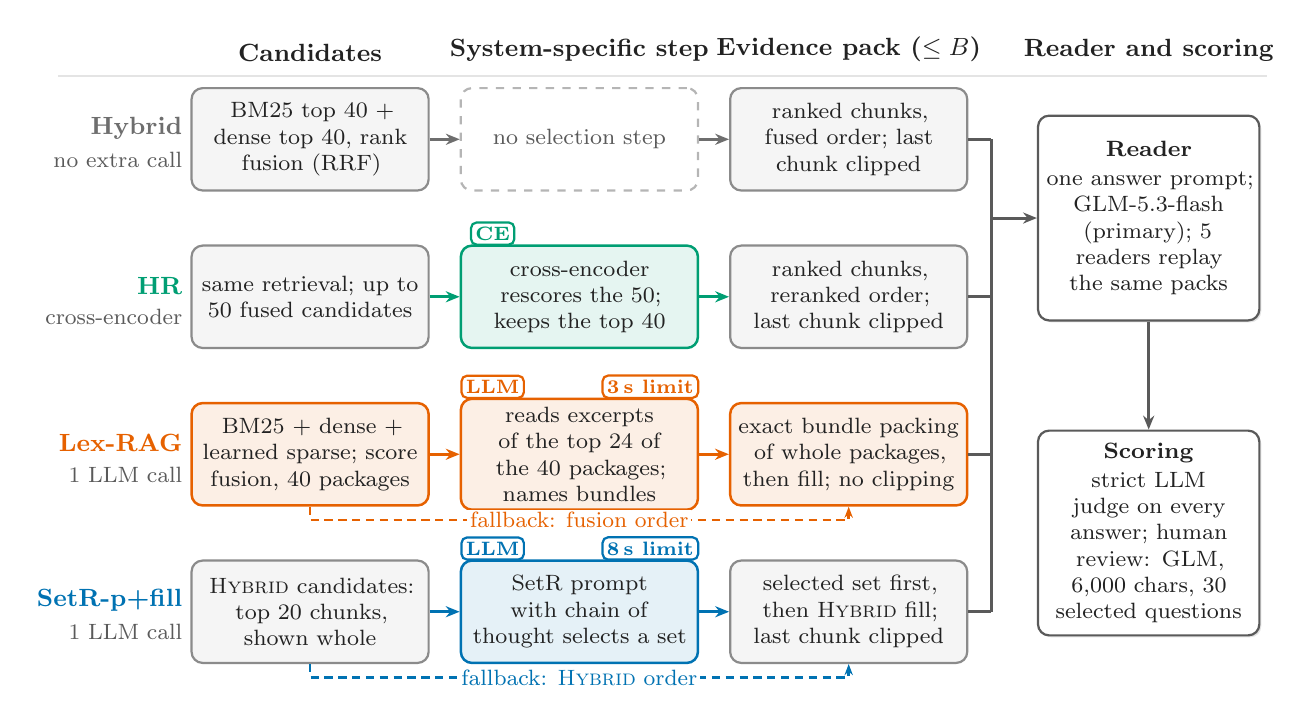
\begin{tikzpicture}[
  x=1cm, y=1cm,
  box/.style={stage=#1, text width=2.8cm, minimum height=1.3cm},
  neutral/.style={draw=cAxis!70, line width=0.8pt, rounded corners=4pt, fill=black!4, align=center, font=\footnotesize,
    inner sep=3pt, text width=2.8cm, minimum height=1.3cm, text=cInk},
  ghost/.style={draw=cAxis!45, line width=0.8pt, dashed, rounded corners=4pt, align=center, font=\footnotesize,
    inner sep=3pt, text width=2.8cm, minimum height=1.3cm, text=cAxis},
  head/.style={font=\small\bfseries, text=cInk, anchor=south},
  tag/.style={draw=#1, fill=white, line width=0.8pt, rounded corners=2pt, font=\scriptsize\bfseries, text=#1,
    inner sep=1.6pt},
]
\def\cA{3.30}\def\cB{6.72}\def\cC{10.14}\def\cD{13.95}
% ---------------------------------------------------------------- column headers
\node[head] at (\cA,0.86) {Candidates};
\node[head] at (\cB,0.86) {System-specific step};
\node[head] at (\cC,0.86) {Evidence pack ($\le B$)};
\node[head] at (\cD,0.86) {Reader and scoring};
\draw[cGrid, line width=0.6pt] (0.1,0.8) -- (15.45,0.8);
% ---------------------------------------------------------------- lane labels
\foreach \y/\c/\n/\s in {0/cHyb/\hybrid/no extra call, -2.0/cHR/\hr/cross-encoder, -4.0/cLex/\lexb/1 LLM call, -6.0/cSetR/\setr/1 LLM call}{
  \node[lanelabel=\c] at (1.8,\y+0.14) {\n};
  \node[font=\footnotesize, text=cAxis, anchor=east] at (1.8,\y-0.26) {\s};
}
% ---------------------------------------------------------------- candidates
\node[neutral] (r1) at (\cA,0)     {BM25 top 40 + dense top 40, rank fusion (RRF)};
\node[neutral] (r2) at (\cA,-2.0) {same retrieval; up to 50 fused candidates};
\node[box=cLex] (r3) at (\cA,-4.0) {BM25 + dense + learned sparse; score fusion, 40 packages};
\node[neutral] (r4) at (\cA,-6.0) {\hybrid{} candidates: top 20 chunks, shown whole};
% ---------------------------------------------------------------- system-specific step
\node[ghost] (s1) at (\cB,0) {no selection step};
\node[box=cHR] (s2) at (\cB,-2.0) {cross-encoder rescores the 50; keeps the top 40};
\node[box=cLex] (s3) at (\cB,-4.0) {reads excerpts of the top 24 of the 40 packages; names bundles};
\node[box=cSetR] (s4) at (\cB,-6.0) {SetR prompt with chain of thought selects a set};
\node[tag=cHR]   at (s2.north west) [xshift=0.42cm, anchor=south, yshift=-0.5pt] {CE};
\node[tag=cLex]  at (s3.north west) [xshift=0.42cm, anchor=south, yshift=-0.5pt] {LLM};
\node[tag=cSetR] at (s4.north west) [xshift=0.42cm, anchor=south, yshift=-0.5pt] {LLM};
\node[tag=cLex]  at (s3.north east) [xshift=-0.62cm, anchor=south, yshift=-0.5pt] {3\,s limit};
\node[tag=cSetR] at (s4.north east) [xshift=-0.62cm, anchor=south, yshift=-0.5pt] {8\,s limit};
% ---------------------------------------------------------------- packing
\node[neutral] (p1) at (\cC,0)     {ranked chunks, fused order; last chunk clipped};
\node[neutral] (p2) at (\cC,-2.0) {ranked chunks, reranked order; last chunk clipped};
\node[box=cLex] (p3) at (\cC,-4.0) {exact bundle packing of whole packages, then fill; no clipping};
\node[neutral] (p4) at (\cC,-6.0) {selected set first, then \hybrid{} fill; last chunk clipped};
% ---------------------------------------------------------------- flows
\foreach \i/\c in {1/cHyb,2/cHR,3/cLex,4/cSetR}{
  \draw[flow=\c] (r\i) -- (s\i);
  \draw[flow=\c] (s\i) -- (p\i);
}
% fallbacks: a missed time limit or an unusable reply skips the selection
\draw[fallback=cLex] (r3.south) -- ++(0,-0.17) -| node[pos=0.25, fill=white, inner sep=1pt, font=\footnotesize, text=cLex] {fallback: fusion order} (p3.south);
\draw[fallback=cSetR] (r4.south) -- ++(0,-0.17) -| node[pos=0.25, fill=white, inner sep=1pt, font=\footnotesize, text=cSetR] {fallback: \hybrid{} order} (p4.south);
% ---------------------------------------------------------------- shared reader and scoring
\node[shared, text width=2.6cm, minimum height=2.6cm] (reader) at (\cD,-1.0)
  {\textbf{Reader}\\[1pt] one answer prompt; GLM-5.3-flash (primary); 5 readers replay the same packs};
\node[shared, text width=2.6cm, minimum height=2.6cm] (judge) at (\cD,-5.0)
  {\textbf{Scoring}\\[1pt] strict LLM judge on every answer; human review: GLM, 6,000 chars, 30 selected questions};
\coordinate (bus) at (11.95,0);
\foreach \i in {1,2,3,4}{\draw[line width=1.1pt, cAxis] (p\i.east) -- (p\i.east -| bus);}
\draw[line width=1.1pt, cAxis] (p1.east -| bus) -- (p4.east -| bus);
\draw[flow] (bus |- reader.west) -- (reader.west);
\draw[flow] (reader) -- (judge);
\end{tikzpicture}
\caption{The four pipelines. They share chunking, an answer prompt and a maximum evidence budget $B$; coloured boxes mark steps specific to one pipeline. The two LLM selectors fall back on a timeout or unusable reply. Five more readers replay the primary run's packs. Settings are in Table~\ref{tab:settings}.}
\label{fig:pipelines}
\end{figure*}

% src: RAG-Paper-upgrades/ragbench: retrieval/hybrid.py, config.yaml (chunking), approaches/hybrid.py (rerank),
%      approaches/lex5b/{approach,views}.py, approaches/lex8/fusion.py; work/datasets_v2/setr/SETR.md;
%      test_freeze/PROTOCOL.md sec. 2 and 9 (arms, readers, pins). Same values as the R3 systems prose.
\begin{table*}[t]
\centering
\small
\renewcommand{\arraystretch}{1.12}
\begin{tabularx}{\textwidth}{@{}>{\raggedright\arraybackslash}p{2.2cm}>{\raggedright\arraybackslash}p{2.6cm}>{\raggedright\arraybackslash}p{2.9cm}>{\raggedright\arraybackslash}X>{\raggedright\arraybackslash}p{3.3cm}@{}}
\toprule
 & \hybrid & \hr & \lexb & \setr \\
\midrule
Channels & BM25, dense & BM25, dense & BM25, dense, learned sparse & BM25, dense \\
Candidates & top 40 per channel; equal-weight RRF & top 50 fused, rescored; top 40 packed & top 40 per channel; three-signal score fusion & selection over \hybrid's top 20 full chunks \\
Extra step & -- & cross-encoder bge-reranker-v2-m3 (local GPU, no LLM tokens) & one selector call over excerpts of the top 24 units: at most 8 parts, at most 2 bundles per part & one chain-of-thought call with the SetR prompt \\
Deadline / cap & -- & -- & 3\,s / 600 completion tokens & 8\,s / 2,000 completion tokens \\
Packing & fused order; last chunk clipped & reranked order; last chunk clipped & best feasible bundle combination (exact cost, no clipping), then fused units that fit whole & selected set first, filled from \hybrid's top 40; clipped \\
On failure & -- & -- & fusion order (\emph{fallback pack}) & \hybrid{} order \\
\midrule
Shared & \multicolumn{4}{>{\raggedright\arraybackslash}p{13.0cm}}{1,000-character chunks (200 overlap); budgets $B\in\{6{,}000;\,15{,}500\}$ rendered characters; one answer prompt per answer format; selector model and primary reader GLM-5.3-flash; five replay readers; judge gpt-oss-120b (Table~\ref{tab:settings-full})} \\
\bottomrule
\end{tabularx}
\caption{The four pipelines and their settings. Further settings, model versions and provider pins are in Appendix~\ref{app:implementation}.}
\label{tab:settings}
\end{table*}


\hybrid{} retrieves chunks with BM25 and with dense bge-m3 vectors \citep{chen2024bgem3} and merges the two rankings by reciprocal rank fusion \citep{cormack2009rrf}. \hr{} rescores the merged list with a cross-encoder reranker, a trained model that scores each passage against the question and needs no LLM tokens. Both fill the budget in ranked order and clip the last chunk if enough of it fits.

\lexb{} has four stages. It first merges BM25, dense and learned-sparse scores into one ranking, which is more sensitive to a strong single signal than rank fusion is. One LLM call then reads short excerpts of the top passages, splits the question into parts and, for each part, names a bundle of passages that together support it. A packer picks the combination of named bundles that covers the most parts within the budget and fills the rest with the next passages, always whole. If the call fails or misses its deadline, the pipeline falls back to the merged ranking.

\setr{} adapts the published SetR selector \citep{lee2025setr}. One chain-of-thought call uses SetR's own prompt to pick a set from \hybrid's candidates. The selected chunks come first and \hybrid's list fills the rest of the budget. Our version uses an untuned selector model and adds the fill, so its results say nothing about the published system.

\label{sec:negative}
\lexb{} is the last of many designs tried on dev, and most variants failed there (Table~\ref{tab:negative-full} in Appendix~\ref{app:negative}). Two findings shaped the final design. First, the three candidate lists together already held a complete gold bundle for 48 of 54 answerable dev questions. Yet the packs of the non-LLM pipelines delivered far fewer, so on dev evidence was lost between candidate list and pack. On the test, more evidence is lost before the candidate list (Section~\ref{sec:lost}). Second, extra query-time lexical search added almost nothing, index-time enrichment did not transfer, and pruning the pack to the selected bundles alone lost evidence the selector had missed. A selection call over good candidates, with a fill, was what remained.

\subsection{Readers and Judge}
\label{sec:readers}
One reader, GLM-5.3-flash, answers every question and also makes both selection calls. Five readers from other model families answer the identical evidence packs, so they add breadth but not independent replications (Table~\ref{tab:settings-full}). We use open models that a deployment without access to the large commercial APIs could run. A pinned LLM judge, which we call the first judge, scores every answer against a strict rubric. An answer counts as correct only if it meets every required point and contains no contradiction, wrong value, wrong subject or unsupported added claim. The judge occasionally returned a reply we could not parse. We leave these 35 of 4,608 answers unscored and report scores as ranges that cover every possible verdict for them. Judge prompts and settings are in Appendix~\ref{app:prompts}.

\subsection{Protocol}
\label{sec:protocol}
Table~\ref{tab:protocol} lists the rules fixed before the test.
% src: work/datasets_v2/test_freeze/PROTOCOL.md (sections 1-10); lex5b/LEX5B.md (token amendment);
%      TEST_RESULTS_HUMAN_SYM.md (symmetric review: 30 questions x 4 pipelines = 120 cells). Same facts as the R3 protocol prose.
\begin{table}[b]
\centering
\small
\renewcommand{\arraystretch}{1.1}
\begin{tabularx}{\columnwidth}{@{}>{\raggedright\arraybackslash}p{1.9cm}>{\raggedright\arraybackslash}X@{}}
\toprule
Element & Rule \\
\midrule
Development & 60 dev questions only; test files never read by the implementing agents (Claude Opus 5.5) \\
Freeze & code commit in the author's repository, manifest of input hashes, pipelines, readers, decision rules; runner refuses any other commit (re-pinned once, at the pre-test re-freeze) \\
Test run & 96 questions $\times$ 8 pipeline--budget cells, each run once; an answered cell is never re-run \\
\midrule
Accuracy gate & \lexb\textsubscript{6000} $\ge$ +5 of 90 against \emph{each} of \hybrid\textsubscript{6000} and \hr\textsubscript{6000} (scaled from +3/54 on dev) \\
Resource gate & \lexb\textsubscript{6000} query-time LLM tokens (selector + reader, reasoning included) $\le 2.5\times$ \hybrid\textsubscript{6000} (relaxed from $1.5\times$ during development) \\
Superiority & two-sided exact sign tests on discordant pairs, Holm-corrected over the two primary comparisons; paired bootstrap intervals \\
Descriptive & \setr, budget effects, other readers, language / genre / tier subgroups \\
\midrule
Unresolved judge cells & reported as identification bounds $a$..$b$; sign-test $p$ as the range over every assignment; intervals clustered by the 20 components of shared source families (all added after the freeze) \\
Human review & after the machine results, blinded to the method: all four 6,000-character pipelines on the 30 machine-discordant questions (120 cells) \\
\bottomrule
\end{tabularx}
\caption{Test protocol. All gates use the primary reader; the machine analysis is primary.}
\label{tab:protocol}
\end{table}

All method development used the dev questions, and Claude Opus 5.5 agents implemented and ran our methods without ever reading the test files. Before the first test answer we froze the code, its inputs and the decision rules, and each test question was run once in every pipeline and budget. The freeze is a commit in our repository; it was not registered with a third party.

Two gates and two tests were fixed in advance, all for the primary reader. An \emph{accuracy gate} required \lexb{} at 6,000 characters, which we call the tight budget, to beat each control, \hybrid{} and \hr, by at least 5 of the 90 answerable questions. A \emph{resource gate} limited its query-time LLM tokens. Two superiority tests covered the main comparisons, and everything else was descriptive. The protocol changed in a few places during development and after the test, mostly in operations, scoring and review. The most important change relaxed the token limit of the resource gate from 1.5 to 2.5 times \hybrid's tokens, before any \lexb{} result. Appendix~\ref{app:timeline} lists every change with its date and its timing relative to the results.

After the machine results were known, the author reviewed answers blinded to the pipeline. The review covers every question on which the four 6,000-character pipelines received different judge verdicts, and all four pipelines on each such question, 30 questions in all. We call the result the \emph{symmetric merge}, because all four pipelines were reviewed on every selected question (an earlier, uneven review is described in Section~\ref{sec:stability}). On those questions the human verdicts replace the judge's, and on all others the judge's verdicts stand. The merge was built after the machine results were known, so it is post hoc.


\section{Results and Discussion}
\label{sec:results}
\phantomsection\label{sec:discussion}
% src: test_run/TEST_RESULTS.md (machine), test_run/TEST_RESULTS_HUMAN_SYM.md (symmetric human), paper/analysis/revision_stats.md
%      (bounds, sign-p ranges, CIs, readers, clipping, tokens), dev60/DEV60.md, setr/SETR.md, budget_matrix/BUDGET_MATRIX.md;
%      power: posthoc_2026-11/S5_stats/RESULTS.md sec. 2.3 (MDE 10.4-11.1 points of 90; power 18-19% for 5/90); TOST: S5 sec. 2.2
% src (rules moved here from the head of 4.2, REVIEW2 item 18): 576 of 576 rebuilt packs byte-identical: S2a_packs/RESULTS.md sec. 1 step 0 and sec. 5 item 1 (6 arms x 96 questions); families of 6 to 13 pairs: S10 12, S11 7, S12 13, S13 6 (RESULTS.md paired sections).
% Rewrite 2026-11-10: Section 4 opens with the confirmatory test; post hoc subsections follow.

The results come in two kinds. The frozen test is the only confirmatory part, because its hypotheses, prompts and decision rules were fixed before any test answer was seen. The remaining subsections use the same test set after its answers were known, to compare retrieval components, to ask why the frozen test came out as it did, to compare the two languages, and to turn the results into guidance. They are post hoc.

All post hoc subsections follow the same rules. Prompts and settings were fixed on dev or a priori, and each new arm was run once on the test questions. The rebuilt evidence packs match the frozen ones byte for byte (576 of 576). We release the ledger of every call, and Appendix Table~\ref{tab:posthoc-log} lists every post hoc arm, including those not discussed here. Because the same 90 answerable questions were used after their answers were known, post hoc $p$-values are descriptive. Each experiment compared a declared family of 6 to 13 pairs. Unless noted, scores are for the primary reader and the first judge, on the 90 answerable questions.

\subsection{Confirmatory Test}
\label{sec:frozen}
% src (post hoc paragraph, REVIEW2 item 16): merged scores 71, 76, 76, 78 and the setr-hybrid 7/0 p .016 = TEST_RESULTS_HUMAN_SYM.md; equivalence at 8: S5_stats sec. 2.2; power and 400 to 460 questions: S5_stats sec. 2.3.
Table~\ref{tab:main} gives accuracy in all eight pipeline and budget cells for the primary reader, and Table~\ref{tab:paired} in Appendix~\ref{app:stats} gives every paired statistic.
% src: work/datasets_v2/test_run/TEST_RESULTS.md sec. 2 and 4 (machine, tokens, latency);
%      work/datasets_v2/test_run/TEST_RESULTS_HUMAN_SYM.md sec. 1 (SYMMETRIC human adjudication, /90: 71/76/76/78;
%      supersedes the asymmetric 68/73/76/72). Ranges a-b = needs_adjudication bounds.
%      fa/en token split: paper/analysis/revision_stats.md (tokens, total|fa, total|en).
% R4: cost columns (tok/q, x HYBRID, p50, p95) moved unchanged to tables/cost.tex.
\begin{table*}[t]
\centering
\small
\setlength{\tabcolsep}{5pt}
\begin{tabular}{@{}llcc|ccccc@{}}
\toprule
 & & \multicolumn{2}{c|}{Correct /90} & \multicolumn{5}{c}{Machine judge, by subgroup} \\
Budget & Pipeline & Machine & Sym.\ merge & fa/45 & en/45 & T1/30 & T2/30 & T3/30 \\
\midrule
\multirow{4}{*}{6,000} & \hybrid & 62--63 & 71 & 35--36 & 27 & 28 & 20--21 & 14 \\
 & \hr & 69--71 & 76 & 36 & 33--35 & 28 & 23--24 & 18--19 \\
 & \lexb & 68--69 & 76 & 36--37 & 32 & 29 & 23--24 & 16 \\
 & \setr & 63 & 78 & 33 & 30 & 27 & 18 & 18 \\
\midrule
\multirow{4}{*}{15,500} & \hybrid & 68 & -- & 35 & 33 & 28 & 22 & 18 \\
 & \hr & 69--70 & -- & 38 & 31--32 & 28 & 21--22 & 20 \\
 & \lexb & 67 & -- & 36 & 31 & 28 & 20 & 19 \\
 & \setr & 66--67 & -- & 35 & 31--32 & 28 & 22--23 & 16 \\
\bottomrule
\end{tabular}
\caption{Test accuracy with the primary reader (GLM-5.3-flash) on the answerable questions. \emph{Machine}: pinned strict judge, $a$--$b$ are bounds over unresolved judge cells. \emph{Sym.\ merge}: symmetric merge (Section~\ref{sec:protocol}), in which the author's verdicts replace the judge's on the 30 questions where the pipelines differed; this column was added after the test; -- = no human review. Subgroup columns are machine scores. Every pipeline abstained correctly on all unanswerable questions.}
\label{tab:main}
\end{table*}


The gate failed. At the tight budget, \lexb{} answered 5 to 7 more of the 90 answerable questions than \hybrid{} under the machine judge and 0 to 3 fewer than \hr. It therefore missed the required margin over \hr, and neither primary test was significant. The confidence intervals, which resample groups of questions that share a source, remain compatible with no improvement. The resource gate passed only under the token limit we relaxed during development; under the original limit it would have failed (Appendix Table~\ref{tab:cost}).

The tiers show where the pipelines can differ (Table~\ref{tab:main}). Single facts (T1) are near ceiling for every pipeline, so a selection step has little room to help there. On within-document questions (T2), \lexb{} and \hr{} gain over \hybrid, while \setr{} does not. On cross-document questions (T3), \hr{} and \setr{} lead. By language, \lexb's gain over \hybrid{} is visible in English and small in Persian.

Development results also shrank on the test, as expected for a method adapted to dev over many iterations. \lexb's lead over \hybrid{} roughly halved from dev to test, and its lead over \hr{} disappeared (Appendix Table~\ref{tab:devtest}). The confirmatory result is therefore a null with a wide interval and says little about which setup to prefer.

Three post hoc checks help read this result. The first is the symmetric merge, in which the author's verdicts replace the judge's on the 30 reviewed questions. It raises every score but does not change the conclusion. \hybrid, \hr, \lexb{} and \setr{} then answer 71, 76, 76 and 78 of 90. All three pipelines with a reranking or selection step have higher point estimates than \hybrid. \lexb{} ties \hr, and its difference from \hybrid{} is not significant once the several comparisons are corrected. \setr{} has the highest merged score; its lead over \hybrid{} (7 wins, no loss, $p=.016$) is one of six uncorrected comparisons. None of the selection pipelines is clearly better than \hr. The second check is an equivalence test on the machine scores, which fails to show that \lexb{} and \hr{} are equivalent even for a margin of 8 questions out of 90.

The third check is a power calculation. With 90 answerable questions and the disagreement rate we observed, a paired comparison has 80\% power only for differences of about 11 answers. A difference of 5, our gate, would be detected in fewer than one case in five, and would need about 400 to 460 questions. The gate was likely to fail whether or not selection helps, and its failure is weak evidence either way. The next subsections use the same test set to ask which retrieval components matter and then why the pipelines differ.

\subsection{Retrieval Components}
\label{sec:components}
% src: posthoc_2026-11/S7_analysis/RESULTS.md sec. 5 (channels.json, Table channels in Appendix: gold recall in the top 40 per channel; fa 37/37/39 complete bundles, items 85/95/99 of 106; en 29/31/37, items 88/96/105 of 124;
%      BM25 normalisation ablation 35 vs 37 complete in fa; 27 of 45 Persian questions contain Persian digits); chunking: A_benchmark.tex (1,000 characters, 200 overlap)
% src: S10_retrieval/RESULTS.md sec. 2.1-2.4, 3, 6 (DENSE_6000 53, BM25_6000 48, HYBRID_6000 62..63, HR_6000 69..71; 15,500: 63, 61, 68; Bonferroni family of 12; discordant on 31 of 90; either-channel oracle 66; top-40 complete bundles dense 71, BM25 66, hybrid 72; packs 47 vs 57;
%      T1 complete bundles in top 40: BM25 30/30, dense 28/30; T3 correct 14 vs 9; statutes 20 vs 17; fa 27 and 24 vs 35..36, en 26 and 24 vs 27)
% src: S11_rewrite/RESULTS.md sec. 2, 5 (HYDE 61, MQ 58..59, HYBRID 62..63; nets -2..-1 and -5..-3; complete bundles 51, 54 vs 57; fa complete 26 and 28 vs 33; fa nets -5..-4 and -7..-5, en +3 and +2; one extra LLM call, +220 to +335 tokens)
% src: S12_chunks/RESULTS.md sec. 2, 5 (HYBRID 58-59/62-63/49, HR 62/69-71/51; HR_C2000 vs HR net -20..-18, 2/20, p <= .0001; mean items in pack 11.5, 6.7, 3.7; last item cut in 73 and 71 of 96 packs at 2,000; complete bundle in top 40: 79-80 vs 72-75; T1 26-28 at every size)
% src: S13_embed/RESULTS.md sec. 2, 5 (E5-HYBRID 58 vs 62..63, net -5..-4, p .18-.34, all Persian; E5-DENSE 54..55 vs 53; complete bundle in top 40: 72 vs 72 hybrid, 69 vs 71 dense; HR beats E5-HYBRID by 11..13)
% src: comparison families: S10 12, S11 7 listed, S12 13 listed, S13 6 (RESULTS.md paired sections). Detectable difference about 11 of 90: S5_stats sec. 2.3.
% src: 576 of 576 rebuilt packs byte-identical: S2a_packs/RESULTS.md sec. 1 step 0 and sec. 5 item 1 (6 arms x 96 questions).
% src (REVIEW2 items 19-23, 2026-11-11): dense exact top-40 38/6/1 (98 of 106 items) fa and 33/11/1 (104 of 124) en = S10_retrieval/RESULTS.md sec. 2.4 and S15_crossling/RESULTS.md sec. 2 X; T1 correct BM25 26 vs dense 24 of 30 and T3 14 vs 9: S10_retrieval/RESULTS.md sec. 2.3; dense minus BM25 +5 p .47: S10 sec. 2.2.
% src (number check 2026-11-11): Persian complete bundles in the top 40, BM25 37 and dense 38 = exact lists, S10_retrieval/RESULTS.md sec. 2.4 and S15_crossling/RESULTS.md sec. 2 X (same as tab:language); S7 tab:channels gives dense 37 as a lower bound.

The frozen test compared whole pipelines, but a practitioner also chooses the parts. This subsection varies four of them one at a time, namely the retrieval channel, query rewriting, chunk size and the embedding model. Each variation changes one part of plain \hybrid{} or \hr{} at a 6,000-character budget. Table~\ref{tab:components} lists every arm.
% src: correct /90, fa/en, complete-bundle reach (S7 gold_reach on the reader messages) and nets (w/l = wins/losses of the arm over resolved pairs):
%      S10_retrieval/RESULTS.md sec. 2.1-2.4 (DENSE, BM25 at 6,000 and 15,500; HYBRID_6000 62..63, fa 35..36, en 27, reach 57; HR_6000 69..71, fa 36, en 33..35, reach 63; HYBRID_15500 68, fa 35, en 33, reach 65),
%      S11_rewrite/RESULTS.md sec. 2 (HYDE 61, MQ 58..59, reach 51 and 54), S12_chunks/RESULTS.md sec. 2 (C500, C2000 for HYBRID and HR; reach 55, 46, 59, 51),
%      S13_embed/RESULTS.md sec. 2 (E5-HYBRID 58, E5-DENSE 54..55, reach 53 and 46; E5-DENSE vs S10 DENSE_6000 +1..+2, 10/8). HR vs HYBRID +6..+9 (10/4): S12 sec. 2 and revision_stats.
\begin{table*}[t]
\centering
\small
\setlength{\tabcolsep}{4pt}
\begin{tabular}{@{}lrrrrr@{}}
\toprule
 & Correct & Persian & English & Complete bundle & Net vs.\ reference \\
Arm & of 90 & of 45 & of 45 & in pack, of 90 & (w/l) \\
\midrule
\multicolumn{6}{@{}l}{\emph{References, 6,000 characters}} \\
\hybrid{} (BM25 and bge-m3, 1,000-character chunks) & 62--63 & 35--36 & 27 & 57 & -- \\
\hr{} (\hybrid{} and cross-encoder) & 69--71 & 36 & 33--35 & 63 & +6..+9 (10/4) \\
\midrule
\multicolumn{6}{@{}l}{\emph{Retrieval channel (reference: \hybrid{} at the same budget)}} \\
Dense only, 6,000 characters & 53 & 27 & 26 & 47 & $-$10..$-$9 (7/16) \\
BM25 only, 6,000 characters & 48 & 24 & 24 & 45 & $-$15..$-$14 (2/16) \\
\hybrid{}, 15,500 characters & 68 & 35 & 33 & 65 & -- \\
Dense only, 15,500 characters & 63 & 34 & 29 & 62 & $-$5 (4/9) \\
BM25 only, 15,500 characters & 61 & 33 & 28 & 59 & $-$7 (1/8) \\
\midrule
\multicolumn{6}{@{}l}{\emph{Query rewriting (reference: \hybrid{}, 6,000 characters)}} \\
HyDE passage & 61 & 31 & 30 & 51 & $-$2..$-$1 (8/9) \\
Multi-query & 58--59 & 29--30 & 29 & 54 & $-$5..$-$3 (6/9) \\
\midrule
\multicolumn{6}{@{}l}{\emph{Chunk size (reference: the same pipeline with 1,000-character chunks)}} \\
\hybrid{}, 500-character chunks & 58--59 & 33 & 25--26 & 55 & $-$5..$-$3 (3/7) \\
\hybrid{}, 2,000-character chunks & 49 & 29 & 20 & 46 & $-$14..$-$13 (3/16) \\
\hr{}, 500-character chunks & 62 & 34 & 28 & 59 & $-$9..$-$7 (4/11) \\
\hr{}, 2,000-character chunks & 51 & 27 & 24 & 51 & $-$20..$-$18 (2/20) \\
\midrule
\multicolumn{6}{@{}l}{\emph{Embedding model (multilingual-e5-large in place of bge-m3)}} \\
\hybrid{} with e5 (reference: \hybrid{}) & 58 & 31 & 27 & 53 & $-$5..$-$4 (2/7) \\
e5 dense only (reference: bge-m3 dense only) & 54--55 & 29 & 25--26 & 46 & +1..+2 (10/8) \\
\bottomrule
\end{tabular}
\caption{Post hoc. Retrieval components varied one at a time at a 6,000-character budget unless stated (GLM-5.3-flash reader, machine judge, 90 answerable questions). Net is the arm minus its reference in answers; w/l counts questions where the arm is right and the reference wrong, and the reverse. Ranges cover unresolved judge cells; comparisons are uncorrected, and each experiment declared 6 to 13 comparisons beforehand.}
\label{tab:components}
\end{table*}


\emph{Retrieval channel.} We start with what each channel finds, before any reader is involved (Table~\ref{tab:channels} in Appendix~\ref{app:posthoc}). Among the top 40 candidates, BM25 and dense retrieval find a complete evidence bundle for 37 and 38 of the 45 Persian questions. Dense retrieval finds more of the individual gold passages (98 of 106 against 85). English shows the same pattern, with a somewhat larger dense advantage. Computed exactly over both languages, the dense list holds a complete bundle for 71 of the 90 questions and the BM25 list for 66. BM25 also depends on text normalisation. Without the tokenizer-level normalisation it loses two complete Persian bundles. The reason is that 27 of the 45 Persian questions contain Persian digits, which only the normalised path matches against the ASCII digits of the corpus.

Recall is not accuracy, so we also ran each channel alone through the same packer and reader. Hybrid retrieval beats both at 6,000 characters, with 62 to 63 correct answers against 53 for dense retrieval and 48 for BM25. The gap to BM25 survives correction over the 12 declared comparisons. The gap to dense retrieval (9 to 10 answers) does not, and it is below the detectable difference. Both single channels fall well below the reranked pipeline. The channels disagree on 31 of the 90 questions, and an oracle that took whichever channel was right would answer 66. BM25 is slightly ahead on single facts (26 against 24 correct of 30) and dense retrieval on cross-document questions (14 against 9). Fusion helps through ordering and not through recall. The dense list holds a complete bundle for almost as many questions as the hybrid list (71 against 72). Its 6,000-character pack does so less often (47 against 57), because fusion moves the chunks that both channels like to the front. A larger budget removes most of the gap, and at 15,500 characters the single channels reach 63 and 61 against 68 for hybrid retrieval. The loss from dropping one channel is larger in the Persian half than in the English half (Section~\ref{sec:language}).

\emph{Query rewriting.} A rewritten query can reach passages that the user's wording misses. We tested two common rewrites, a hypothetical answer passage written by an LLM before retrieval (HyDE \citep{gao2023hyde}) and three paraphrases of the question whose results are merged (multi-query). Neither helped. HyDE scored 61 and multi-query 58 to 59, against 62 to 63 for the unrewritten query, and both stay well below the reranker. Each costs one extra LLM call per question. Rewriting also lowered the number of questions for which a complete evidence bundle reached the reader, and the loss was concentrated in Persian (26 and 28 of 45 against 33). In English the two rewrites were a few answers better than no rewrite, which is within noise. Rewriting gave no gain, and in the Persian half it lowered both accuracy and the number of complete bundles.

\emph{Chunk size.} Our pipelines cut documents into chunks of at most 1,000 characters. We repeated the retrieval with chunks of 500 and 2,000 characters at the same 6,000-character budget. Chunks of 1,000 characters were best for both \hybrid{} and \hr. Chunks of 2,000 characters lose clearly, by 13 to 14 answers for \hybrid{} and 18 to 20 for \hr. The loss happens at packing and not at retrieval. The top 40 list held a complete bundle for more questions with large chunks than with the standard size. But only about four large chunks fit into the pack, against about seven standard ones, and the last was cut in most packs. Chunks of 500 characters cost a few answers, and for \hybrid{} this cannot be told from no change. At both other sizes the reranker's gain over plain \hybrid{} shrinks. The losses come almost entirely from the within-document and cross-document tiers, since single-fact questions are near ceiling at every size.

\emph{Embedding model.} The dense channel so far uses bge-m3 \citep{chen2024bgem3}. We swapped in multilingual-e5-large to see whether the conclusions depend on that choice. Used alone, the two dense models tie, with 54 to 55 correct answers for e5 and 53 for bge-m3. Inside hybrid retrieval, e5 scored 58 against 62 to 63. That gap of four or five answers is not significant, and all of it lies in the Persian questions. The candidate lists are alike, because either hybrid holds a complete bundle in its top 40 for 72 of the 90 questions, so any difference comes from ordering. Swapping the embedding model therefore changes little.

Together these experiments leave the default where it was. Two changes cost more than the detectable difference of about 11 answers, namely using BM25 alone and using 2,000-character chunks, and none improved on plain hybrid retrieval with 1,000-character chunks. The next subsections ask what happens to the candidates on their way to the reader.

% src: posthoc_2026-11/S2a_packs/RESULTS.md (FUSION, GOLD, MMR, KNAP; sec. 2.1, 2.2, 2.4), S6_baselines (CLOSEDBOOK 26, LISTWISE 66-67, SETR_NOFILL 63),
%      S2b_variance (selector swap 59; fallbacks), S7_analysis/RESULTS.md (reach table, contamination, 16/16, 64 vs 53),
%      S8_factorial/tables.md (SELHR 70, LEX5B_NODL 71-72, dev replication +8 9/1; RESULTS.md not yet written when this was drafted), S1_evaluator (judge 2)
% All scores: machine judge 1, primary reader, 90 answerable questions, 6,000 characters unless stated.
% src (judge 2, added 2026-11-11): S8_factorial/tables.md 'Accuracy, judge 2' (FUSION_6000 57..59, LEX5B_6000 65..67; gap 6..10); S14_bilingual compact_table.md (Lex-RAG vs FUSION @6000 under judge 2: fa +4, en +2..+6); SELHR and LEX5B_NODL were not sent to judge 2 (absent from that table).

% src (REVIEW2 N1/N2, 2026-11-11): funnel counts of Table funnel = S10_retrieval/RESULTS.md sec. 2.4 (top-40 complete: BM25 66, dense 71, hybrid 72, HR 75; packs 45, 47, 57, 63) and S7_analysis/RESULTS.md sec. 1 reach table (packs Lex-RAG 64, Lex-RAG without selection 53, ITER_BM25 71)
%      and sec. 5 (Lex-RAG F2 top 40: 40 + 35 = 75; Lex-RAG without selection uses the same 40 candidates); correct: S2a_packs, S8_factorial/tables.md, S10. Losses: 90-75 = 15 to 90-72 = 18 before the list; 72-57 = 15, 75-63 = 12, 75-64 = 11 in packing.
%      Selector effect: +9..+11 saved answers (S8_factorial/results.json acc_j1, LEX5B_6000 vs FUSION_6000); redraws +4..+6 and +4..+5 (S14_bilingual/RESULTS.md sec. 2.1 'replicates r1; r2', sum of the halves: fa +2..+3 / en +2..+3 and fa +3..+4 / en +1);
%      second judge +6..+10 (S8_factorial/tables.md 'Accuracy, judge 2': FUSION_6000 57..59, LEX5B_6000 65..67; S8_factorial/RESULTS.md sec. 3.1 is stale, tables.md is the source); dev +8, 9 wins 1 loss (S8_factorial dev_fusion; E_posthoc).
%      Listwise 66..67 vs LEX5B 68..69 (S6_baselines); HR 69..71 vs LEX5B 68..69 (S2a_packs).

\subsection{Where Answers Are Lost and What Selection Adds}
\label{sec:lost}
This subsection asks where wrong answers come from and which step of \lexb{} matters. The rules of Section~\ref{sec:results} apply, and scores are for 6,000 characters unless noted.

We first check whether the reader is the problem, then trace each miss to the evidence the reader saw, and finally ask which step in \lexb{} makes the difference.

\subsubsection{Reader Ability}
Two reference runs bracket what the reader can do. In the \emph{closed book} run it gets no evidence and answers from memory. In the \emph{gold evidence} run it gets only the first annotated bundle, about 570 characters. Closed book it answers 26 of the 90 questions. With the gold bundle it answers 83, including every within-document question. The best single-pass pipelines reach 70 to 72, even at four times the budget. Most of the remaining gap therefore lies in what the pipelines put in front of the reader.

The closed-book run also tests the benchmark itself. Company-report questions are never answered from memory, but many English book and statute questions are. Those 26 questions are partly contaminated by the reader's training data. We therefore repeated the main contrasts without them. The gain of \lexb{} over \hybrid{} is as large without these questions, so it does not depend on them.

\subsubsection{Evidence in the Pack}
% src: figures/data/lost_arms.dat, written by paper/analysis/figure_data_posthoc.py from work/posthoc_2026-11/S7_analysis/reach.json
%      (S7 task 1: exact reader messages parsed; a gold item "reached" the reader if >= 90% of its quote occurs in the pack
%      items of its own document; complete = every item of one annotated bundle, partial = some, none = no item).
\newcommand{\lostx}{0}
\newcommand{\lostseg}[4]{% value, fill, text colour, y
  \pgfmathsetmacro{\lostxe}{\lostx+#1}%
  \ifnum#1>0
    \fill[#2] ({\lostx*0.112},{#4-0.21}) rectangle ({\lostxe*0.112},{#4+0.21});
    \ifnum#1>2 \node[font=\footnotesize, text=#3, inner sep=0pt] at ({(\lostx+\lostxe)/2*0.112},{#4}) {#1};\fi
  \fi
  \xdef\lostx{\lostxe}}
\begin{figure*}[t]
\centering
\pgfplotstableread{figures/data/lost_arms.dat}\losttab
\begin{tikzpicture}
\foreach \r in {0,...,8}{
  \pgfplotstablegetelem{\r}{lab}\of\losttab \edef\vlab{\pgfplotsretval}
  \pgfplotstablegetelem{\r}{hc}\of\losttab \edef\vhc{\pgfplotsretval}
  \pgfplotstablegetelem{\r}{hp}\of\losttab \edef\vhp{\pgfplotsretval}
  \pgfplotstablegetelem{\r}{hn}\of\losttab \edef\vhn{\pgfplotsretval}
  \pgfplotstablegetelem{\r}{un}\of\losttab \edef\vun{\pgfplotsretval}
  \pgfplotstablegetelem{\r}{mn}\of\losttab \edef\vmn{\pgfplotsretval}
  \pgfplotstablegetelem{\r}{mp}\of\losttab \edef\vmp{\pgfplotsretval}
  \pgfplotstablegetelem{\r}{mc}\of\losttab \edef\vmc{\pgfplotsretval}
  \pgfplotstablegetelem{\r}{rc}\of\losttab \edef\vrc{\pgfplotsretval}
  \pgfmathsetmacro{\yy}{-0.58*\r}
  \xdef\lostx{0}
  \node[font=\footnotesize, text=cInk, anchor=east] at (-0.15,\yy) {\vlab};
  \lostseg{\vhc}{cHit}{cInk}{\yy}
  \lostseg{\vhp}{cHit!60!white}{cInk}{\yy}
  \lostseg{\vhn}{cHit!28!white}{cInk}{\yy}
  \lostseg{\vun}{black!35}{white}{\yy}
  \lostseg{\vmn}{cMiss!30!white}{cInk}{\yy}
  \lostseg{\vmp}{cMiss!65!white}{cInk}{\yy}
  \lostseg{\vmc}{cMiss}{white}{\yy}
  \node[font=\footnotesize\bfseries, text=cInk, anchor=west] at ({92*0.112},\yy) {\vrc};
}
\draw[cAxis, line width=0.5pt] (0,-5.15) -- ({90*0.112},-5.15);
\foreach \t in {0,20,40,60,80}{\draw[cAxis, line width=0.5pt] ({\t*0.112},-5.15) -- ({\t*0.112},-5.25) node[below, font=\footnotesize, text=cInk, inner sep=2pt] {\t};}
\node[font=\footnotesize, text=cInk, anchor=north] at ({45*0.112},-5.65) {answerable questions (of 90)};
\node[font=\footnotesize\bfseries, text=cInk, anchor=south west] at ({92*0.112-0.55},0.38) {complete};
\node[font=\footnotesize, text=cInk, anchor=south west] at ({92*0.112-0.55},0.16) {bundle};
% key
\begin{scope}[font=\footnotesize, text=cInk, shift={(0,1.0)}]
  \node[anchor=west] at (-4.1,0) {\textbf{Correct:}};
  \fill[cHit] (-2.75,-0.09) rectangle (-2.45,0.09); \node[anchor=west, inner sep=2pt] at (-2.45,0) {all};
  \fill[cHit!60!white] (-1.55,-0.09) rectangle (-1.25,0.09); \node[anchor=west, inner sep=2pt] at (-1.25,0) {part};
  \fill[cHit!28!white] (-0.2,-0.09) rectangle (0.1,0.09); \node[anchor=west, inner sep=2pt] at (0.1,0) {none};
  \fill[black!35] (1.2,-0.09) rectangle (1.5,0.09); \node[anchor=west, inner sep=2pt] at (1.5,0) {unresolved};
  \node[anchor=west] at (4.0,0) {\textbf{Wrong:}};
  \fill[cMiss!30!white] (5.2,-0.09) rectangle (5.5,0.09); \node[anchor=west, inner sep=2pt] at (5.5,0) {none};
  \fill[cMiss!65!white] (6.5,-0.09) rectangle (6.8,0.09); \node[anchor=west, inner sep=2pt] at (6.8,0) {part};
  \fill[cMiss] (7.8,-0.09) rectangle (8.1,0.09); \node[anchor=west, inner sep=2pt] at (8.1,0) {all};
\end{scope}
\end{tikzpicture}
\caption{Post hoc. Where the answers are lost (GLM-5.3-flash, 90 answerable questions). Bars split each arm's questions by judged correct (blue) or wrong (orange) and by how much gold evidence was in the reader's pack; the number at right counts questions with a complete bundle. Packs are 6,000 characters, except the two search agents, which may show up to 15,500.}
\label{fig:lost}
\end{figure*}

To see why answers fail, we checked for every question whether the annotated evidence appears in the pack the reader received (Figure~\ref{fig:lost}). A question is \emph{complete} if some full evidence bundle is in the pack, \emph{partial} if only some of the needed passages are, and \emph{none} if nothing is. At 6,000 characters the pattern is the same for every pipeline. Most misses are partial, because the pack held part of the evidence but not all of it. Few misses have no evidence at all, and a few have a complete bundle.

Evidence is lost at two points (Table~\ref{tab:funnel}). The first is before the candidate list exists. The top 40 candidates hold a complete bundle for 72 questions with hybrid retrieval, 71 with dense retrieval, 66 with BM25 and 75 with the reranked list and with the fusion used by \lexb. For 15 to 18 of the 90 questions the evidence is therefore gone at retrieval. The second is packing. The 6,000-character packs hold a complete bundle for 57 questions (\hybrid), 63 (\hr) and 64 (\lexb), a further loss of 11 to 15. For plain hybrid retrieval the two losses are about equal, and for the reranked pipeline the retrieval loss is the larger (15 against 12). The reference run with gold evidence answers 83, so even a complete bundle does not guarantee a correct answer.
% src: S10_retrieval/RESULTS.md sec. 2.4 'Gold-bundle coverage' (top-40 list and delivered 6,000-character pack: BM25 66 and 45, dense 71 and 47, hybrid 72 and 57, HR 75 and 63, of 90);
%      S7_analysis/RESULTS.md sec. 1 (packs: Lex-RAG 64, Lex-RAG without selection 53, GOLD 90 complete) and sec. 5 (Lex-RAG F2 top 40 = 40 + 35 = 75, also the candidates of Lex-RAG without selection);
%      correct of 90 (machine judge 1): S10 (BM25 48, dense 53), S2a_packs/S8_factorial tables.md (hybrid 62..63, HR 69..71, Lex-RAG without selection 58..59, Lex-RAG 68..69, gold 83).
\begin{table}[t]
\centering
\footnotesize
\setlength{\tabcolsep}{4pt}
\begin{tabular}{@{}lccc@{}}
\toprule
 & \multicolumn{2}{c}{Complete bundle} & Correct \\
\cmidrule(lr){2-3}
Pipeline & Top 40 & Pack & answers \\
\midrule
BM25 & 66 & 45 & 48 \\
Dense & 71 & 47 & 53 \\
\hybrid{} & 72 & 57 & 62--63 \\
\hr{} & 75 & 63 & 69--71 \\
Lex-RAG without selection & 75 & 53 & 58--59 \\
\lexb{} & 75 & 64 & 68--69 \\
Gold evidence (reference) & -- & 90 & 83 \\
\bottomrule
\end{tabular}
\caption{Post hoc. Questions out of 90 whose top 40 candidates hold a complete gold evidence bundle, whose 6,000-character pack holds one, and that were answered correctly. The gold evidence row gives the first annotated bundle only, so its pack is complete by construction.}
\label{tab:funnel}
\end{table}


Of the wrong answers that had a complete bundle, the reviewer accepted all 16 that were reviewed. These are disagreements between the judge and the reviewer and not failures of the pipeline (Section~\ref{sec:stability}). The cross-document tier is where bundles are most often partial, and 22 questions received a complete bundle from none of the single-pass pipelines at 6,000 characters. They are most often cross-document questions, and the iterative BM25 agent, which issues new queries, recovers them best (71 complete bundles). Figure~\ref{fig:examples} shows one case of the effect of selection. In a Persian report question about drivers' income, the reply of the selector added the definition of full-time work that Lex-RAG without selection lacked.

\subsubsection{Role of the Selection Call}
% src: correct /90 and tokens: work/posthoc_2026-11/S2a_packs/results.json (table: HYBRID_6000, HR_6000, FUSION_6000, KNAP_6000, MMR_6000, GOLD;
%      LEX5B_6000 and net bounds in `compare`), S3_agentic/results.json (LEX5B_6000 4,511..5,131 and SETR_6000 7,503..8,128 tokens/q),
%      S6_baselines/analysis.json (CLOSEDBOOK 199+118 tokens, LISTWISE 6,774+254, SETR_NOFILL 1,170+114 answer plus the saved SETR
%      selector call 5,060+221 = 6,565; selector usage unknown for 6 SETR fallback calls; `paired` for nets), S2b_variance/results.json (exp3: selector swap).
%      Net = arm minus reference, in answers of 90, bounds over unresolved judge cells; w/l = wins/losses of the arm over resolved pairs.
%      Hybrid and HR rows against Lex-RAG are the negation of LEX5B_6000 vs HYBRID_6000 (+5..+7, 11/4) and vs HR_6000 (-3..0, 6/7), revision_stats.json.
% Net vs. HYBRID for gold (83 - 62..63 = +20..+21) and for selection over the reranker's candidates (70 - 62..63 = +7..+8) = differences of totals (S8_factorial/tables.md accuracy judge 1); win/loss counts were not computed.
% S8_factorial/RESULTS.md sec. 2.3-2.4, results.json acc_j1: LEX5B_NODL_6000 (71..72; vs HYBRID +8..+10, 13/4; vs LEX5B_6000 +2..+4, 3/1), SELHR_6000 (70; vs LEX5B_6000 +1..+2, 7/6; vs HR_6000 -1..+1, 9/8). Tokens not itemised for these arms.
\begin{table*}[t]
\centering
\small
\setlength{\tabcolsep}{5pt}
\begin{tabular}{@{}lrrcrr@{}}
\toprule
 & Correct & LLM tokens & LLM & Net vs.\ & Net vs.\ \\
Arm & of 90 & per question & calls & \hybrid{} (w/l) & \lexb{} (w/l) \\
\midrule
\multicolumn{6}{@{}l}{\emph{References}} \\
Closed book (no evidence) & 26 & 317 & 1 & $-$37..$-$36 (8/44) & -- \\
\hybrid{} & 62--63 & 2,216 & 1 & -- & $-$7..$-$5 (4/11) \\
\hr{} (cross-encoder reranker) & 69--71 & 2,237 & 1 & +6..+9 (10/4) & 0..+3 (7/6) \\
\lexb{} & 68--69 & 4,511--5,131 & 2 & +5..+7 (11/4) & -- \\
Gold evidence (first annotated bundle) & 83 & 481 & 1 & +20..+21 & +14..+15 (17/3) \\
\midrule
\multicolumn{6}{@{}l}{\emph{Selection removed or replaced}} \\
\lexb{} without selection & 58--59 & 2,150 & 1 & $-$5..$-$3 (3/6) & $-$11..$-$9 (2/12) \\
MMR packer, same candidates & 60 & 2,158 & 1 & $-$3..$-$2 (4/6) & $-$9..$-$8 (3/11) \\
Knapsack packer, same candidates & 44 & 2,116 & 1 & $-$19..$-$18 (3/21) & $-$25..$-$24 (3/28) \\
\lexb{} with a different selector model & 59 & -- & 2 & $-$4..$-$3 (9/12) & $-$10..$-$9 (3/13) \\
\lexb{} without the 3-second deadline & 71--72 & -- & 2 & +8..+10 (13/4) & +2..+4 (3/1) \\
Selection over the reranker's candidates & 70 & -- & 2 & +7..+8 & +1..+2 (7/6) \\
\midrule
\multicolumn{6}{@{}l}{\emph{Other selection methods}} \\
\setr{} & 63 & 7,503--8,128 & 2 & 0..+1 (8/7) & $-$6..$-$5 (4/10) \\
SetR, selected set only (no fill) & 63 & 6,565 & 2 & 0..+1 (10/9) & $-$6..$-$5 (6/12) \\
Listwise LLM reranker & 66--67 & 7,028 & 2 & +3..+5 (12/7) & $-$3..$-$1 (7/9) \\
\bottomrule
\end{tabular}
\caption{Post hoc. Effect of the selection step at 6,000 characters (GLM-5.3-flash reader, machine judge, 90 answerable questions). Net is the arm minus the reference in answers; w/l counts questions where the arm is right and the reference wrong, and the reverse. Ranges cover unresolved judge cells; comparisons are uncorrected. Net without w/l is a difference of totals. Tokens were not itemised for arms marked --.}
\label{tab:ablation}
\end{table*}

If missing evidence is the main cause, the selection call should be the step that matters. Table~\ref{tab:ablation} tests this by removing or replacing it. Lex-RAG without selection uses the same fused candidates and the same packer, but no LLM call. Against \lexb's saved answers it scores 9 to 11 answers lower. When the \lexb{} side is replaced by either of two later reader redraws, the difference is 4 to 6 and 4 to 5 answers (Table~\ref{tab:variance}). A second judge gives 6 to 10, and the 54 answerable dev questions give 8 (9 wins, 1 loss). We therefore read the effect as about 5 to 10 answers at 6,000 characters. The loss shows in both languages. With the call, a complete bundle reaches the reader on 64 questions, against 53 without it. Without the call, \lexb{} is no better than \hybrid, so its fusion and packing give no measurable gain alone.

Packers without an LLM do not replace the call. An embedding-based diversity rule (MMR) and a score-per-character knapsack score well below \lexb. A listwise LLM reranker, which reorders \hybrid's top 20 in one call, comes within three answers of \lexb{} (66 to 67 against 68 to 69) and stays below \hr. A smaller selector model cuts \lexb{} to the level of Lex-RAG without selection, because its replies often broke the required format and the pipeline fell back to the pack without selection. Lifting the selector's 3-second deadline changes \lexb's score by at most a few answers.

A cross-encoder does as well with less. \hr{} scores as high as \lexb{} (69 to 71 against 68 to 69) with no LLM tokens, while \lexb{} needs about twice \hybrid's tokens. Applying \lexb's selection call to \hr's reranked candidates is no better than \hr{} alone. Once a cross-encoder has ordered the candidates, the selection call adds no measurable gain. The selected set also need not be large. \setr's selected set alone, about three chunks and 3,000 characters, scores the same as its set plus fill at half the characters.

At 6,000 characters the pipelines differ mainly in what they pack. Their candidate lists hold a complete bundle for a similar number of questions (71 to 75 of 90), and a reranking or selection step, whether an LLM call or a cross-encoder, is what moves accuracy. A second judge points the same way. It scores Lex-RAG without selection at 57 to 59 and \lexb{} at 65 to 67, a gap of 6 to 10 answers against 9 to 11 under the first judge. The gap is present in both languages. The second judge did not score the arms with the selector over the reranker's candidates or without a deadline.

\subsection{Effect of the Evidence Budget}
\label{sec:evidence}
\phantomsection\label{sec:budget}
% src: posthoc_2026-11/S2a_packs/RESULTS.md sec. 2.1, 2.3 (HYBRID/HR/FUSION at 3k-24k; tokens/q), S8_factorial/tables.md (LEX5B at 3k/10k/24k; RESULTS.md not yet written when drafted),
%      S2b_variance sec. 2.5 (shared selection: budget effect ~0), S7_analysis sec. 3 (1.80x marginal ratio; token-matched view; SETR_NOFILL vs 3000),
%      S5_stats sec. 2.1 (budget effects in the pooled model; no budget x reader terms, p .55-.81), S3_agentic cost table (tokens/q)
% All scores: machine judge 1, primary reader, 90 answerable questions.
% src (REVIEW2 N2, 2026-11-11): HR 15,500 vs 6,000 = -2..+1 on the saved draw; redraws r1 65 -> 70..71 and r2 67..68 -> 73 = +5..+6 (S2b_variance/RESULTS.md sec. 2.1 table, rows HR_6000 and HR_15500); five other readers +1 to +12 (Table readers, Budget effect HR column);
%      pooled OR HR 1.61 p .076, hybrid 1.77, Lex-RAG 1.13 (Table glmm = S5_stats/tables.md); HR_24000 66 (S8_factorial/tables.md). Selection call +15..+16 (3,000), +9..+11 (6,000), +3..+4 (10,000), +2 (15,500, 24,000): S8_factorial/tables.md paired comparisons;
%      redraws +4..+6 and +4..+5: S14_bilingual/RESULTS.md sec. 2.1; second judge +6..+10: S8_factorial/tables.md (RESULTS.md sec. 3.1 is stale); Lex-RAG without selection at 3,000 = 43..44 vs HYBRID_3000 49..51; Lex-RAG_3000 59, HR_3000 56: S8_factorial/tables.md accuracy judge 1.
%      Token-matched view (+4..+7 hybrid and +6..+8 HR at 3,000; +2..+5 and -2..0 at 6,000): S7_analysis/RESULTS.md sec. 3, Table tokens.

The error analysis showed that a reranking or selection step matters at 6,000 characters. We next vary the budget, because with a large enough pack choosing may matter less. We ran the pipelines at five budgets from 3,000 to 24,000 characters (Figure~\ref{fig:budget}). Only the 6,000 and 15,500 points are the frozen ones.
% src: figures/data/budget.dat, written by paper/analysis/figure_data_posthoc.py from work/posthoc_2026-11/S2a_packs/results.json
%      (table: acc90 bounds, query_tokens_all_mean). Hybrid, HR and Lex-RAG without selection at five budgets, GLM-5.3-flash, judge 1;
%      Lex-RAG at 6,000 and 15,500 (frozen cells) and at 3,000, 10,000, 24,000 (S8_factorial/results.json acc_j1; the saved 6,000-character selector reply
%      re-packed at each budget). Token position of the three new Lex-RAG points = S2a Lex-RAG-without-selection tokens of that budget plus the selection call (LEX5B_6000 minus FUSION_6000 tokens).
\begin{figure*}[t]
\centering
\begin{tikzpicture}
\begin{axis}[paper, name=left, width=7.4cm, height=5.6cm, xmin=1, xmax=25.5, xtick={3,6,10,15.5,24}, xticklabels={3,6,10,15.5,24},
  ymin=40, ymax=76, ytick={40,45,...,75}, ymajorgrids, xlabel={Evidence budget (thousand characters)}, ylabel={Correct of 90},
  title={Characters shown to the reader}]
\pgfplotsinvokeforeach{1,2,5,3}{%
  \addplot[pcls#1, forget plot, mark=none, line width=1.1pt, restrict expr to domain={\thisrow{cls}}{#1:#1}] table[x expr=\thisrow{budget}/1000, y=mid] {figures/data/budget.dat};
  \addplot[pcls#1, restrict expr to domain={\thisrow{cls}}{#1:#1}, ybound] table[x expr=\thisrow{budget}/1000, y=mid, y error minus expr=\thisrow{mid}-\thisrow{lo}, y error plus expr=\thisrow{hi}-\thisrow{mid}] {figures/data/budget.dat};
  \addplot[pcls#1, only marks, forget plot, restrict expr to domain={\thisrow{cls}}{#1:#1}] table[x expr=\thisrow{budget}/1000, y=mid] {figures/data/budget.dat};
}
\end{axis}
\begin{axis}[paper, at={(left.east)}, anchor=west, xshift=1.1cm, width=7.4cm, height=5.6cm, xmin=0.5, xmax=11, xtick={2,4,6,8,10},
  ymin=40, ymax=76, ytick={40,45,...,75}, yticklabels={}, ymajorgrids, xlabel={Query-time LLM tokens per question (thousands)},
  title={Tokens spent (all calls)}]
\pgfplotsinvokeforeach{1,2,5,3}{%
  \addplot[pcls#1, forget plot, mark=none, line width=1.1pt, restrict expr to domain={\thisrow{cls}}{#1:#1}] table[x=tok, y=mid] {figures/data/budget.dat};
  \addplot[pcls#1, restrict expr to domain={\thisrow{cls}}{#1:#1}, ybound] table[x=tok, y=mid, y error minus expr=\thisrow{mid}-\thisrow{lo}, y error plus expr=\thisrow{hi}-\thisrow{mid}] {figures/data/budget.dat};
  \addplot[pcls#1, only marks, forget plot, restrict expr to domain={\thisrow{cls}}{#1:#1}] table[x=tok, y=mid] {figures/data/budget.dat};
}
\end{axis}
\node[font=\footnotesize, anchor=south] at ($(left.north east)+(0.55cm,0.75cm)$) {\pkey{cHyb}{*}{\hybrid}\quad\pkey{cHR}{square*}{\hr}\quad\pkey{cLex}{triangle*}{\lexb}\quad\pkey{cFus}{pentagon*}{\lexb{} without selection}};
\end{tikzpicture}
\caption{Post hoc. Accuracy at five evidence budgets (left) and against tokens spent per question (right). Bars show the range over unresolved judge cells. \lexb{} counts the selection call; at 3,000, 10,000 and 24,000 characters it reuses the selection made at 6,000.}
\label{fig:budget}
\end{figure*}


The curves differ by pipeline. Plain \hybrid{} rises steadily, from about 50 correct answers at 3,000 characters to 72 at 24,000. The reranked pipeline \hr{} gets most of its accuracy from the first 6,000 characters. On the saved answers of the primary reader it is flat from 6,000 to 15,500 ($-$2..+1) and lower at 24,000 (66). That is one reader draw. Two later redraws of the same packs put 15,500 characters five or six answers above 6,000, the five other readers gain 1 to 12 answers, and the pooled odds ratio is 1.61 ($p=.076$, Table~\ref{tab:glmm}). The reranked pipeline therefore gains less from a bigger pack than hybrid retrieval does on the saved draw, but not reliably so, and its drop at 24,000 lies within reader noise. Lex-RAG without selection follows \hybrid's shape. \lexb{} itself is flat between 6,000 and 15,500 and then reaches \hybrid's level at 24,000. At the largest budget the differences among \hybrid, \lexb{} and Lex-RAG without selection are negligible. The reranking and selection steps therefore pay mainly at small budgets, and plain retrieval catches up when it is shown several times as much text.

That catch-up has a price in tokens. \hybrid{} needs 15,500 characters to match \lexb's 6,000-character score. Its reader prompt is then as long as the total query tokens of \lexb, which spends a second call on selection (Appendix Table~\ref{tab:cost}). A cross-encoder gets the same accuracy from the 6,000-character pack with less than half of those tokens. A bigger budget is thus an alternative to selection, and it has a cost. \lexb's curve stays flat when one selector reply is packed at both budgets, so the flatness is not an effect of separate selector calls.

Persian makes the budget harder to set. A character costs the primary reader about 1.8 times as many tokens in Persian as in English, so the same character budget is a larger token budget in Persian. Section~\ref{sec:language} gives the ratio for six readers. If the two languages get equal tokens, English packs hold about 1.8 times the characters. This raises accuracy most at 3,000 characters (4 to 8 answers). At 6,000 characters the gain is 2 to 5 answers for \hybrid{} and gone for \hr{} (Appendix Table~\ref{tab:tokens}).

% src: S8_factorial/RESULTS.md, results.json (Lex-RAG vs Lex-RAG without selection: +15..+16 at 3k, 17/2, p<=.0007; +9..+11 at 6k; +3..+4 at 10k; +2 at 15.5k and 24k)
% src (judge 2 coverage): S8_factorial/tables.md "Accuracy, judge 2" (all eight frozen 6,000 and 15,500 cells from S1; no 3,000/10,000/24,000 cell); S14_bilingual/RESULTS.md sec. 1 (HYBRID_3000, LEX5B_3000, FUSION_3000, HYBRID_24000 never sent to judge 2)
The selection call has its clearest effect at the smallest budget. Packing the same selector reply at every budget shows how its value fades as the pack grows. At 3,000 characters \lexb{} answers 15 to 16 more questions than Lex-RAG without selection, at 6,000 characters 9 to 11 on the saved answers (4 to 6 with either of two reader redraws, and 6 to 10 under the second judge), and from 10,000 characters on only 2 to 4. The 3,000-character figure is one run, with no redraw and no second-judge score. The comparison pack is also 6 answers below plain hybrid retrieval at that budget (43 to 44 against 49 to 51). Against the alternatives a practitioner has, \lexb{} at 3,000 characters answers 8 to 10 more than \hybrid{} and 3 more than \hr{} (59 against 49 to 51 and 56).

\setr's selected set, about 3,000 characters, answers 12 to 14 more questions than \hybrid{} at a 3,000-character budget. It does not significantly beat \hr{} at that budget. Pooling all six readers, the budget effect is positive for \hybrid{} and \hr{} (odds ratios 1.77 and 1.61) and near zero for \lexb{} (1.13). Nothing in the pooled model suggests that this depends on the reader (Section~\ref{sec:stability}). The budget curves rest on the first judge alone, since a second judge scored only the 6,000- and 15,500-character arms.

\subsection{Iterative Retrieval, Long Context and Routing}
\label{sec:search}
% src: posthoc_2026-11/S3_agentic/RESULTS.md (ITER_BM25 73, GREP_AGENT 68, tokens 4.19x/5.57x, English +12, T3 +7/+9, evidence chars median 2,735/1,652, 17 comparisons),
%      S4_route_long/RESULTS.md (LC-GOLD-DOCS 79, LC-BM25-DOCS 24, LC-POOL, routing: oracle -> HR_15500 69..70 with 21% fewer tokens, GLM router 66/90 correct routes),
%      S7_analysis/RESULTS.md sec. 2 (ITER_BM25 vs HR_6000 -1..0 without the 26 closed-book-correct questions)
% src: S9_gpu/RESULTS.md sec. 2 (HYBRID_AGENT 77/90; fa 39, en 38; vs HR_6000 +6..+8, 15/8, p .15-.31; vs HYBRID_6000 +14..+15; without the 26: 55/64 vs 50-51, vs HYBRID +10..+11 p .013-.031; 9,070 tokens, 3.62 calls, median latency 10.5 s vs 3.2 s HR; gain over ITER_BM25 is Persian +5)

% src (REVIEW2 items 38-41, 2026-11-11): BM25 agent vs HR on the 26 memory-answerable questions +3..+4 (4/1) and on the other 64 -1..0: S7_analysis/contam_tables.md (Table contam); hybrid agent vs hybrid +14..+15 and vs HR +6..+8: S9_gpu/RESULTS.md sec. 2; HR_6000 2,237 tokens and routers 4,153 to 5,065: S3_agentic/results.json, S4_route_long/routing_tables.md (Table search); HR_6000 69..71 vs HR_15500 69..70: S3_agentic/results.json.
If a single pass loses evidence, spending more effort might recover it. We tested three ways of doing so, namely an iterative search agent, reading whole documents, and routing questions to a cheaper or dearer pipeline (Table~\ref{tab:search}).
% src (T3 column, REVIEW2 N3, 2026-11-11): cross-document correct of 30: HR_6000 18..19, HR_15500 20, LEX5B_6000 16, ITER_BM25 23, GREP_AGENT 21 = S8_factorial/tables.md accuracy judge 1; hybrid-index agent 25 = S9_gpu/RESULTS.md sec. 2 table; -- = not tabulated.
% src: S3_agentic/results.json arms and paired (ITER_BM25, GREP_AGENT: accuracy, fa/en, tokens_per_q, calls_per_q; vs HR_6000 in results_tables.md);
%      S4_route_long/lc_tables.md and lc_results.json (LC-GOLD-DOCS, LC-BM25-DOCS: accuracy, tokens_per_q_mean, comparisons vs HR_6000),
%      S4_route_long/routing_tables.md (oracle and GLM-router rows, format rule: accuracy, tokens/q, calls/q; "vs always HR_6000");
%      frozen rows from S3 results.json (HR_6000, LEX5B_6000, HR_15500). Net = arm minus HR at 6,000 characters, bounds over unresolved judge cells.
\begin{table*}[t]
\centering
\small
\setlength{\tabcolsep}{4.5pt}
\resizebox{\textwidth}{!}{%
\begin{tabular}{@{}lrrrrrrr@{}}
\toprule
 & Correct & Persian & English & Cross-doc. & LLM tokens & LLM & Net vs.\ \hr{} \\
Arm & of 90 & of 45 & of 45 & (T3, of 30) & per question & calls & 6,000 (w/l) \\
\midrule
\multicolumn{8}{@{}l}{\emph{Best single-pass pipelines}} \\
\hr{}, 6,000 characters & 69--71 & 36 & 33--35 & 18--19 & 2,237 & 1.0 & -- \\
\hr{}, 15,500 characters & 69--70 & 38 & 31--32 & 20 & 5,287 & 1.0 & -- \\
\lexb{}, 6,000 characters & 68--69 & 36--37 & 32 & 16 & 4,511--5,131 & 2.0 & $-$3..0 (6/7) \\
\midrule
\multicolumn{8}{@{}l}{\emph{Search agents (up to five rounds, 15,500-character answer pack)}} \\
BM25 search agent & 73 & 34 & 39 & 23 & 9,285 & 3.6 & +2..+4 (11/8) \\
Hybrid-index search agent (reranker) & 77 & 39 & 38 & 25 & 9,070 & 3.6 & +6..+8 (15/8) \\
Grep agent & 68 & 29 & 39 & 21 & 12,338 & 5.1 & $-$3..$-$1 (12/13) \\
\midrule
\multicolumn{8}{@{}l}{\emph{Long context (32,000-token prompt)}} \\
Gold documents (uses the annotation) & 79 & 37 & 42 & -- & 29,569 & 1.0 & +8..+10 (17/8) \\
BM25-ranked documents & 24 & 11 & 13 & -- & 30,967 & 1.0 & $-$47..$-$45 (2/48) \\
\midrule
\multicolumn{8}{@{}l}{\emph{Routing between a cheap and a wide pipeline}} \\
By gold tier (uses the annotation), to \hr{} at 15,500 & 69--70 & 38 & 31--32 & -- & 4,167 & 1.0 & $-$2..+1 (6/5) \\
By a language-model router, to \hr{} at 15,500 & 68--69 & 38 & 30--31 & -- & 5,065 & 2.0 & $-$3..0 (6/6) \\
By answer format, to \hr{} at 15,500 & 67--68 & 37 & 30--31 & -- & 4,153 & 1.0 & $-$4..$-$1 (5/6) \\
\bottomrule
\end{tabular}}
\caption{Post hoc. Search agents, long-context reading and routing against the best single-pass pipelines (GLM-5.3-flash reader, machine judge, 90 answerable questions). Each arm ran once; tokens count every call; ranges cover unresolved judge cells; comparisons are uncorrected.}
\label{tab:search}
\end{table*}


The iterative agents have the best point estimates. Each agent is the same GLM model. It may search the question's pool up to five times, then names the passages it wants the reader to see. With BM25 as its only search tool the agent scores 73 of 90, against 69 to 71 for \hr{}, and uses about four times \hybrid's tokens. With the full hybrid index and the cross-encoder as its search tool it scores 77, the highest of any arm that does not use the annotations. The token cost is the same, and the median latency is 10.5 seconds against 3.2 for \hr. That is 14 or 15 answers more than \hybrid, but only 6 to 8 more than \hr, a difference the test cannot separate from noise. The gain over the BM25 agent lies in Persian (39 of 45 against 34), and over the single-pass pipelines it lies mostly in cross-document and English questions. The agents also hand over little text. The passages they pass on average about 3,000 characters, well below the budget they were allowed.

The BM25 agent's lead depends on questions the reader can answer without any evidence. Of the 90 questions, 26 are answered correctly in the closed-book run. Against \hr{}, the BM25 agent wins 4 of those 26 questions and loses 1 (Table~\ref{tab:contam}). On the other 64 the two are level (the agent is behind by one answer at most), so without the questions the reader answers from memory it shows no measurable advantage over a cross-encoder. Its search tool is also weaker than the pipelines' own, since it uses BM25 only, with no dense retrieval and no reranker. The hybrid-index agent keeps part of its lead without them. It answers 55 of the 64, against 50 to 51 for \hr{}, and 10 to 11 more than \hybrid{} (uncorrected sign test, $p$ between .013 and .031). Its lead over \hr{} stays within noise, with or without the memory-answerable questions.

A second agent searches the raw documents with regular expressions and reads the surrounding text. It costs more still (about 5.6 times \hybrid's tokens), scores 68, and does no better than \hybrid{} with 15,500 characters. Persian-aware text normalisation did not rescue it on Persian questions.

Reading whole documents does not help unless the right documents are known. With the gold documents given, 30 thousand tokens of text arranged around the gold passages let the reader answer 79 questions. This is an upper reference that no deployed system can reach. Without that knowledge, the best-matching documents by BM25, cut to the same length, give 24. A gold document was present for almost every question, but the cut text kept only a quarter of the gold passages. Only the two statute pools fit the reader's context window at all, and a whole-pool prompt costs about 210 times the tokens of a \hybrid{} question.

Routing questions by difficulty has nothing to gain on this test. \hr{} at 6,000 characters already scores as high as \hr{} at 15,500 (69 to 71 against 69 to 70), at fewer tokens (2,237) than any router (4,153 to 5,065). An oracle that sent single-fact questions to the cheapest path and the rest to \hr{} at 15,500 characters would save 21 percent of the tokens of always using that wider pipeline. A router that has to guess from the question text sent only 8 of the 30 single-fact questions to the cheap path, so it saved 4 percent. The expected answer format, which every pipeline already receives, is a better difficulty signal. It is derived from the annotation, so we do not count it as a deployable router.

The BM25 agent comparisons are a family of 17 tests, and none survives correction for multiplicity. The hybrid-index agent comparisons were run later and are uncorrected. The reading is therefore modest. More search costs several times the tokens and is slower. The hybrid-index agent is 14 to 15 answers above plain hybrid retrieval, more than the detectable difference of the test, and 6 to 8 above the reranker, which is not.

\subsection{Persian and English}
\label{sec:language}
% src: posthoc_2026-11/S14_bilingual/RESULTS.md sec. 2.1-2.4, 5 and compact_table.md, lang_tables.md (replication; interaction tests; MDE; tokens per character for six readers);
%      S15_crossling/RESULTS.md sec. 2, 5 (cross-lingual query swap: BM25 2/45 and 8/45 complete bundles, dense 35 and 28; hybrid below dense; HR_6000_TRANS 53..54 vs 69..71, 4/20, p .001-.004; closed book 18/45 and 4..5/45; orthography);
%      S6_baselines/RESULTS.md sec. 2 (closed book 20/45 English, 6/45 Persian, reports 0/30), S7_analysis sec. 2 (26 questions answered from memory: 9 English books, 11 English statutes, 3 Persian books, 3 Persian statutes);
%      S7_analysis sec. 3 (1.80x); S10_retrieval sec. 2.3 (fa 27 and 24 vs 35..36 for single channels, en 26 and 24 vs 27); S11_rewrite sec. 2 (fa -5..-4 and -7..-5, en +3 and +2); S13_embed sec. 5 (all of the e5 loss in Persian)

% src (REVIEW2 N5, 2026-11-11): Table language = S15_crossling/RESULTS.md sec. 2 X (fusion packs 33 -> 19 vs dense 26 -> 21, Persian pool; HR packs fa 34 -> 29, en 29 -> 20; fusion en 24 -> 16; top 40 fusion 33 vs dense 35 fa and 27 vs 28 en; BM25 2 and 8; dense loses 3 and 5; end to end 69..71 -> 53..54); 20 of 45 Latin-script names: S15 sec. 2 (en_noLatin = 25 of 45); translator = the reader model (S15 translate.py, GLM-5.3-flash).
The earlier subsections pooled the two languages. This one looks at the halves separately. The two halves use different documents, so a difference between them mixes language and source (Section~\ref{sec:benchmark}). We report what belongs to a language or its tooling, what appears in both halves, and what each question shows when it is asked in both languages.

\emph{Token cost.} Every reader model charges more tokens for a character of Persian evidence than for a character of English (Table~\ref{tab:tokenizers}). For five of the six readers the ratio lies between about 1.5 and 1.8, and for the sixth it is about 3. English costs nearly the same under every tokenizer, so the spread lies on the Persian side. A character budget is therefore not a token budget for any model family we tested. With the primary reader a Persian pack of 6,000 characters costs about as much as an English pack of 10,000.
% src: tab:tokenizers = work/posthoc_2026-11/S14_bilingual/RESULTS.md sec. 2.4 (tokjudge.json tokens: marginal prompt tokens per evidence character, per-language OLS on 768 calls per reader, 8 frozen arms x 96 questions)
% src: tab:language = S15_crossling/RESULTS.md sec. 2 (results_tables.md, experiment X): complete gold bundle in the top 40 and in the 6,000-character pack, original -> translated query, 45 answerable questions per pool;
%      end to end: HR_6000 69..71 -> 53..54 (fa pool 36 -> 28, en pool 33..35 -> 25..26); CLOSEDBOOK 26 -> 22..23 (fa 6 -> 4..5, en 20 -> 18)
% src: tab:replication = S14_bilingual/compact_table.md and lang_tables.md (net A - B per half, GLM reader, judge 1; interaction = worst-case component-level permutation p over unresolved cells; Holm over 14 contrasts for the grep agent: .019)
\begin{table}[t]
\centering
\footnotesize
\setlength{\tabcolsep}{4pt}
\begin{tabular}{@{}p{2.6cm}rrr@{}}
\toprule
Reader & Persian & English & Ratio \\
\midrule
GLM-5.3-flash (primary) & 0.409 & 0.228 & 1.80 \\
DeepSeek-V4-flash & 0.396 & 0.226 & 1.75 \\
Llama 3.3 70B & 0.348 & 0.226 & 1.53 \\
gpt-oss-20b & 0.341 & 0.225 & 1.51 \\
Gemma 3 27B & 0.354 & 0.242 & 1.46 \\
Qwen3 235B & 0.758 & 0.254 & 2.99 \\
\bottomrule
\end{tabular}
\caption{Post hoc. Reader prompt tokens added per character of evidence text, for the six reader models, estimated from 768 answer calls per reader on identical packs. The ratio is Persian over English; 95\% intervals lie within $\pm$0.11.}
\label{tab:tokenizers}
\end{table}

\begin{table}[t]
\centering
\footnotesize
\setlength{\tabcolsep}{2.5pt}
\begin{tabular}{@{}p{3.1cm}cc@{}}
\toprule
Question language swapped & Persian pool & English pool \\
\midrule
\multicolumn{3}{@{}l}{\emph{Complete bundle in the top 40 (of 45), original $\to$ translated}} \\
BM25 & 37 $\to$ 2 & 29 $\to$ 8 \\
Dense & 38 $\to$ 35 & 33 $\to$ 28 \\
Hybrid (rank fusion) & 39 $\to$ 33 & 33 $\to$ 27 \\
Hybrid and reranker & 39 $\to$ 35 & 36 $\to$ 28 \\
\midrule
\multicolumn{3}{@{}l}{\emph{Complete bundle in the 6,000-character pack (of 45)}} \\
BM25 & 25 $\to$ 0 & 20 $\to$ 4 \\
Dense & 26 $\to$ 21 & 21 $\to$ 16 \\
Hybrid (rank fusion) & 33 $\to$ 19 & 24 $\to$ 16 \\
Hybrid and reranker & 34 $\to$ 29 & 29 $\to$ 20 \\
\midrule
\multicolumn{3}{@{}l}{\emph{Correct answers (of 45)}} \\
Reranked pipeline & 36 $\to$ 28 & 33--35 $\to$ 25--26 \\
Closed book & 6 $\to$ 4--5 & 20 $\to$ 18 \\
\bottomrule
\end{tabular}
\caption{Post hoc. Every test question asked in the other language against its own document pool, with the original question in the left value and the translated one in the right. Hybrid retrieval here is BM25 and dense retrieval merged by reciprocal rank fusion.}
\label{tab:language}
\end{table}

\begin{table*}[t]
\centering
\small
\setlength{\tabcolsep}{5pt}
\begin{tabular}{@{}lrrr@{}}
\toprule
 & Persian half & English half & Difference between \\
Contrast (net answers, A minus B) & (of 45) & (of 45) & halves, permutation $p$ \\
\midrule
\lexb{} against Lex-RAG without selection, 3,000 characters & +7..+8 & +8 & 1.00 \\
\lexb{} against Lex-RAG without selection, 6,000 characters & +4..+6 & +5 & 1.00 \\
\hr{} against \hybrid{}, 6,000 characters & 0..+1 & +6..+8 & .17 \\
\hybrid{} at 15,500 against 6,000 characters & $-$1..0 & +6 & .11 \\
SetR set only against \hybrid{}, 3,000 characters & +2..+3 & +10..+11 & .12 \\
Hybrid-index search agent against \hybrid{} & +3..+4 & +11 & .11 \\
BM25 search agent against \hybrid{} & $-$2..$-$1 & +12 & .02 \\
Grep agent against \hybrid{} & $-$7..$-$6 & +12 & .001 \\
Gold evidence against \hr{} & +7 & +5..+7 & 1.00 \\
\bottomrule
\end{tabular}
\caption{Post hoc. Contrasts split by language half, with the primary reader and first judge. The last column tests whether the two halves differ, by permuting the 20 source groups between languages (worst case over unresolved cells). Only the grep agent row survives correction over the 14 contrasts tested (adjusted $p$ = .02). Nine of the 14 contrasts are shown; the other five are in the released analysis tables (S14). Each half has 45 questions and detects a difference of about 8.}
\label{tab:replication}
\end{table*}


\emph{Memory.} With no evidence at all the reader answers 20 of the 45 English questions and 6 of the 45 Persian ones. It answers none of the company-report questions in either language, and the English book and statute questions account for most of its correct answers. This could mean that the model knows English better, or that the English texts, which include classic books and EU law, are better known than the Persian ones. Asking every question in the other language separates the two readings. English-source questions asked in Persian are still answered from memory 18 times out of 45, and Persian-source questions asked in English 4 or 5 times out of 45. The memory gap therefore follows the source texts and not the language of the question. The Persian half is therefore less affected by memorised answers.

\emph{Questions asked in the other language.} The same swap tests retrieval. The reader model translated all 90 answerable questions into the other language, keeping every name and number, and we searched the original pool. Table~\ref{tab:language} gives the result. BM25 collapses, because the query shares few words with the text. It finds a complete evidence bundle in its top 40 for only 2 of 45 Persian-pool questions and 8 of 45 English-pool questions. Those 8 come mostly from Latin-script names that stayed in the Persian translations, which 20 of the 45 translated questions keep. Dense retrieval holds up, losing 3 and 5 bundles. Rank fusion loses the lead it had over dense retrieval. In the Persian pool its pack held a complete bundle for 33 questions against 26 for dense retrieval with the original questions, and for 19 against 21 with the translated ones. A reranker recovers most of the loss in the Persian pool (34 to 29 bundles in the pack, against 33 to 19 for fusion) and little in the English pool (29 to 20, a loss of 9, as large as fusion's 8). Answers fall clearly too. The reranked pipeline answers 53 to 54 of 90 translated questions, against 69 to 71 with the original ones, and the drop is similar in both pools. For questions in another language than the documents, a dense channel is necessary, and rank fusion with BM25 loses its usual advantage.

\emph{Agents with lexical tools.} The search agents split by language. Against plain hybrid retrieval the grep agent gains 12 answers in the English half and loses 6 or 7 in the Persian half. The BM25 agent gains 12 and loses 1 or 2 (Table~\ref{tab:replication}). The grep agent is the only contrast whose difference between the halves survives correction for the 14 contrasts we tested. It also holds without the 26 questions the reader can answer from memory, and against both repeat runs of the hybrid control. The agent with the hybrid index and the reranker gains in both halves, by 3 or 4 answers in Persian and 11 in English. The gain of the lexical agents in the English half did not appear in the Persian half. We do not know whether the cause is Persian itself or the Persian documents.

\emph{Spelling variants.} With normalisation, spelling variants cost at most one complete bundle in the top 40. The exception is the pack, where removing the non-joiner costs even the normalised hybrid three bundles. We rewrote the 45 Persian questions with Arabic letters in place of the Persian ones, with the zero-width non-joiner removed or replaced by a space, and with other digit systems. Without normalisation BM25 loses five to seven bundles under Arabic letters, and eight when all changes are combined, whereas dense retrieval on raw text loses at most one. A hybrid without normalisation keeps its recall because the dense channel compensates, yet fewer complete bundles reach the pack, since the noisy BM25 votes push gold chunks out of it. The normaliser keeps the non-joiner, so removing it merges words. The test questions were already in clean spelling, which is why the earlier ablation (Section~\ref{sec:components}) showed a loss of only two bundles. In practice, normalise before BM25.

\emph{What holds in both halves.} Table~\ref{tab:replication} splits the main contrasts by half. The effect of the selection call has the same sign in both halves at both budgets, with no sign that the halves differ. It is significant only in the English half at 3,000 characters. Every other single-pass effect, namely the reranker over hybrid retrieval, the larger budget and the SetR set, lies mainly in the English half. For none of them is the difference between the halves shown, and after correction no within-half test is significant. With 45 questions a half detects a difference of only about 8 answers, so a result confined to one half may simply be underpowered.

\subsection{Practical Recommendations}
\label{sec:practice}
% src: every claim is taken from Sections 4.1-4.6 and the tables cited in Table guide; the only number not repeated from them is HR against HYBRID at 6,000 characters (+6..+9, 10/4, sign p .049-.18): S12_chunks/RESULTS.md sec. 2 paired table, revision_stats.json.
% src (REVIEW2 N3/N4/N5, 2026-11-11): HR vs HYBRID positive in 9 of 9 pairings of reader draws, mean +6.3..+8.0 (S2b_variance/RESULTS.md sec. 2.3 'HR_6000 vs HYBRID_6000 ... >0 in 9/9'); Persian half 0..+1 and judge 2 HR 63 vs HYBRID 59..61 (S14_bilingual/RESULTS.md sec. 2.1; S8_factorial/tables.md judge 2); pooled p .308 (Table glmm);
%      cross-lingual numbers as in Section 4.6 (S15_crossling sec. 2 X); 77 vs 69..71: S9_gpu/RESULTS.md.
% Confidence wording follows work/review_fable/FRAMING.md: the default is "one choosing step beats none at a tight budget; which step is unresolved".

The earlier subsections gave controlled comparisons. This one turns them into recommendations. Table~\ref{tab:guide} lists common situations and gives the setup we would pick, the evidence behind it and how far that evidence can be trusted. Each row rests on one benchmark, one primary reader and 90 answerable questions, so only large differences count as strong evidence.
% src: Table main (test_run/TEST_RESULTS.md), Table ablation (S2a_packs, S6_baselines, S8_factorial), Table search (S3_agentic, S4_route_long, S9_gpu), Table cost (latency p50),
%      Table channels (S7_analysis sec. 5), Table contam (S7_analysis sec. 2), Figure budget (S2a_packs, S8_factorial), Table components (S10_retrieval, S11_rewrite, S12_chunks, S13_embed),
%      Tables tokenizers, language, replication (S14_bilingual, S15_crossling). Every cell points to the section or table that holds the numbers.
% src (REVIEW2 N3, 2026-11-11): rows re-graded; numbers as in the sections cited; new numbers: 63 vs 59..61 judge 2 (S8_factorial/tables.md), pooled p .308 (S5_stats, Table glmm), -2..+6 (S2b Table variance / Table readers), 55 vs 50..51 of 64 (S9_gpu sec. 2), 4 wins 1 loss (S7 Table contam).
% Confidence: strong = the difference is larger than the ~11 answers the test can detect (about 8 of 45 in one half), or the claim concerns a measured cost or a large retrieval-level effect, or the tier leaves no room for a difference; tentative = same direction in the point estimates but within the noise of 90 questions.
\begin{table*}[t]
\centering
\scriptsize
\setlength{\tabcolsep}{3pt}
\renewcommand{\arraystretch}{1.02}
\begin{tabularx}{\textwidth}{@{}>{\raggedright\arraybackslash}p{2.5cm}>{\raggedright\arraybackslash}p{4.9cm}>{\raggedright\arraybackslash}X>{\raggedright\arraybackslash}p{1.9cm}@{}}
\toprule
Situation & Recommended setup & Why (evidence in this paper) & Confidence \\
\midrule
Single-fact questions (T1) & Hybrid retrieval at a modest budget; no reranker or selection call. & Every pipeline answers 27 to 29 of 30 (Table~\ref{tab:main}). & Strong \\
Within-document questions (T2) & Hybrid retrieval with a cross-encoder reranker. & The reranker and Lex-RAG answer 23 to 24 of 30, plain hybrid 20 to 21 (Table~\ref{tab:main}). & Tentative \\
Cross-document questions (T3) & Reranker first. Add an iterative agent over the hybrid index if four times the tokens and about 10 s are acceptable. & The reranker and SetR lead plain hybrid (18 to 19 against 14 of 30, Table~\ref{tab:main}); the agent reaches 25 of 30 but is not significantly ahead of the reranker (Table~\ref{tab:search}). & Tentative \\
Retrieval channel & Run BM25 and dense retrieval and fuse them. If only one can run, use dense retrieval with a larger budget. & Hybrid 62 to 63, dense 53, BM25 48 at 6,000 characters; at 15,500 the gaps shrink to 5 and 7 (Table~\ref{tab:components}). & Strong against BM25 alone, tentative against dense \\
Chunk size & About 1,000 characters. & Reranked pipeline: 69 to 71 at 1,000, 62 at 500, 51 at 2,000; few large chunks fit the pack (Table~\ref{tab:components}). & Strong against 2,000 at a 6,000-character budget with this packer; tentative against 500 \\
Query rewriting & Do not add HyDE or multi-query. & 61 and 58 to 59 against 62 to 63, at one extra LLM call, and fewer complete bundles in Persian (Section~\ref{sec:components}). & Tentative \\
Embedding model & bge-m3 or multilingual-e5-large; spend effort on a reranker. & Dense-only scores tie; e5 is 4 to 5 lower inside hybrid, not significantly (Table~\ref{tab:components}). & Tentative \\
Persian budgets & Set budgets in tokens, not characters. & Persian costs about 1.5 to 1.8 times the tokens per character for five of six readers, 3.0 for one (Table~\ref{tab:tokenizers}). & Strong \\
Persian spelling and digits & Normalise letters, non-joiners and digits before BM25. & Without normalisation BM25 loses 5 to 8 of 45 complete bundles; retrieval only (Section~\ref{sec:language}). & Tentative \\
Query language differs from the documents & A dense channel, and a reranker after the fusion; not BM25 alone. & BM25 finds 2 and 8 of 45 bundles, dense 35 and 28; fusion loses its lead over dense; the reranked pipeline still answers 53 to 54 against 69 to 71 (Table~\ref{tab:language}). & Strong for the BM25 collapse, tentative for fusion against dense \\
Tight budget (6,000 characters) & A reranking or selection step: a cross-encoder, or an LLM selection call if none is available. & Removing the selection call costs about 15 answers at 3,000 characters (one run) and 5 to 10 at 6,000 (Table~\ref{tab:ablation}, Figure~\ref{fig:budget}). The cross-encoder's lead over plain hybrid (6 to 9) is not significant (pooled $p=.31$; 63 against 59 to 61 under the second judge). & Strong at 3,000 characters for the selection call, one run; tentative at 6,000 characters and for the cross-encoder \\
Loose budget (15,500 characters or more) & Plain hybrid retrieval; reranking and selection add little. & Hybrid rises from about 50 to 72 correct; the reranked pipeline gains less ($-$2 to +6 across reader draws; Figure~\ref{fig:budget}). & Tentative \\
Latency-sensitive & One pass: hybrid, with or without a reranker. No selection calls or agents. & Median latency 1.8 s hybrid, 3.2 s reranked, 4.0 s Lex-RAG, 5.5 s SetR, 10.5 s agent (Tables~\ref{tab:cost} and~\ref{tab:search}); measured under contention, so only the order is informative. & Tentative \\
No GPU for a reranker & Hybrid with a larger budget, or an LLM selection call over the fused candidates. & Hybrid at 15,500 matches Lex-RAG at 6,000 with 2.5 times the text (Figure~\ref{fig:budget}). & Tentative \\
Questions answerable from memory & Do not count on retrieval; build the evaluation without them. & The reader answers 26 of 90 with no evidence (Table~\ref{tab:contam}). & Strong \\
Search agents & Treat the BM25 agent's lead over the reranker with caution. & It lies in the 26 memory-answerable questions (4 wins, 1 loss); the hybrid-index agent keeps a lead without them (55 against 50 to 51 of 64; Table~\ref{tab:contam}). & Tentative \\
\bottomrule
\end{tabularx}
\par\smallskip
{\footnotesize\emph{Note.} Every row rests on 90 answerable questions, one primary reader and one judge. \emph{Strong}: the difference is larger than the test can detect (about 11 answers, or about 8 within one language half) and also holds across the reader draws where they exist, or the claim concerns a measured cost, or the tier leaves no room for a difference. \emph{Tentative}: the point estimates agree but lie within the noise of the test.\par}
\caption{Recommendations for choosing a setup, with the evidence for each and our confidence in it. Post hoc, except the first three rows, which rest on the frozen test (Table~\ref{tab:main}).}
\label{tab:guide}
\end{table*}


The data do not settle one default. At 3,000 characters the selection call has a clear effect against Lex-RAG without selection, but at 6,000 characters neither the cross-encoder nor the selection call beats plain hybrid retrieval significantly on the primary analysis. We suggest hybrid retrieval followed by a cross-encoder reranker as the starting point for two reasons. It needs no LLM tokens, and its difference from plain hybrid retrieval was positive in all nine pairings of reader draws (mean +6 to +8). That difference is not significant, it is absent in the Persian half, and under the second judge it is 2 to 4 answers. Every LLM-based alternative we tried, whether listwise reranking, set selection or the iterative agent, cost two to four times the tokens without a clear gain. The component experiments add to this default. Keep both retrieval channels, cut chunks at about 1,000 characters and skip query rewriting. The choice between the two embedding models we tried does not matter much.

Several steps help only in narrow conditions. An LLM selection call helps when it is the only reranking or selection step. It is therefore the option when no GPU is available for a reranker, but it gives no measurable gain on top of a cross-encoder. Showing more text works in the same case, since plain hybrid retrieval catches up to a selector at about two and a half times the characters. Iterative search over the full hybrid index scores highest (77 against 69 to 71 of 90 for the reranked pipeline). It needs four times the tokens and three times the median latency. Its gain appears mostly on English and cross-document questions, and it is not significant against the reranker. Reading whole documents works only when the right documents are already known. With the gold documents given the reader answers 79 questions, and with the best-matching documents by BM25 it answers 24. A router that had to guess difficulty from the question text saved only 4 percent of the tokens.

For Persian, the recommendations that stand firmest rest on measurements and not on a contrast between the halves. Budgets should be set in tokens, because Persian text costs more tokens per character. Spelling and digits should be normalised before BM25. When the question language differs from the document language, a dense channel is necessary and a reranker should follow the fusion. Even then the best pipeline answers 15 to 18 fewer questions (53 to 54 against 69 to 71). We make no claim that any method works better or worse in Persian as such (Section~\ref{sec:language}).

Two points about evaluation follow from these results. The first is to check the evidence before the reader. Most failures are packs that hold only part of what is needed, so counting complete evidence bundles tells more than accuracy alone. The second is to build the evaluation so that it can detect what matters. Of our 90 questions, 26 can be answered from memory, and the BM25 agent's lead over the reranker lies in those 26. These recommendations are post hoc and need a new test. The next section asks how far the rankings behind them can be trusted.

\section{Robustness Analysis}
\label{sec:stability}
\phantomsection\label{sec:judge}
% src: posthoc_2026-11/S2b_variance/RESULTS.md (reader replicates: SD about 2 of 90, 8-15 of ~89 questions flip; selector re-sent: pack changes 44-50 of 96; SETR re-runs 68),
%      S1_evaluator/RESULTS.md (judge 2: agree 91.2%, kappa 0.760; 6,000 ranking under both judges; judge-human 37/116 and 39/117 stricter, never laxer; 15 vs 9/9/9/12; judge-2 gain is English),
%      S7_analysis/RESULTS.md sec. 4a (66 disagreements: 30 extra unsupported claim, 7 real error, 7 Persian term), sec. 6.1 (15 of 27),
%      S5_stats/RESULTS.md (GLMM OR 2.11 [1.24, 3.60] p .006; vs HR OR 1.61 p .080; no pipeline x reader interaction p .65; TOST; MDE 10-11),
%      TEST_RESULTS_HUMAN_SYM.md (judge-human disagreement), PAPER_ASTRA_R1.log (asymmetric review episode)
% src (REVIEW2 N2c, items 56-61, 2026-11-11): single cells moved by up to six = Table variance (S2b_variance/results.json exp1: LEX5B_6000 68..69 -> 63..64 and 63; SETR_6000 63 -> 68..69 and 68); saved draw five weeks older and 'not exchangeable in the strict sense' = S2b_variance/RESULTS.md sec. 2.1;
%      judge 2 order at 6,000: LEX5B 65..67, SETR 63..65, HR 63, HYBRID 59..61 = S8_factorial/tables.md 'Accuracy, judge 2' (RESULTS.md sec. 3.1 is stale); asymmetric review +8 (9/1, Holm .043) and symmetric +5 (7/2, Holm .359, p .18) = work/datasets_v2/test_run/TEST_RESULTS_HUMAN_SYM.md sec. 'LEX5B_6000 vs HYBRID_6000'; OR 2.11 p .006 = Table glmm (S5_stats).
% src (judge agreement by language): S14_bilingual/RESULTS.md sec. 2.5 and tokjudge.json (judge1_vs_judge2: fa 89.7 percent, kappa 0.690, n 380; en 92.7 percent, kappa 0.817, n 370; difference -0.126, p .21; without LAW-fa-T1-002 0.737; judge 1 rejects 13/37 = 35 percent of human-accepted fa and 24/58 = 41 percent of en; 12 fa and 18 en reviewed questions; disagreement causes 39 fa cells and 27 en cells)
% src (asymmetric first review): work/datasets_v2/test_run/TEST_RESULTS_HUMAN.md sec. 2 (wins 9 vs HYBRID, 8 vs HR) with work/datasets_v2/human_check/key_test.json (cells reviewed): the control was not reviewed in 4 of 9 and 4 of 8 wins (8 of 17, "almost half")

Every comparison above rests on one reader draw, one judge and, for the merged scores, one reviewer. This section checks how far the rankings survive a change in each of these, and then pools all six readers into one model (Figure~\ref{fig:stability}). These checks are also post hoc.
% src: figures/data/stability.dat, written by paper/analysis/figure_data_posthoc.py from
%      work/posthoc_2026-11/S2b_variance/results.json (exp1.cells[arm].acc_by_rep: the saved answers and two more draws of the
%      reader on the identical packs, judge 1), work/posthoc_2026-11/S1_evaluator/judge2_results.json (ranking_6000_ans90:
%      judge 2; symmetric human merge with judge 1 or judge 2 on the 60 questions the human did not review).
%      All values: correct of 90 answerable test questions at 6,000 characters, GLM-5.3-flash; bars = bounds over unresolved cells.
\begin{figure*}[t]
\centering
\begin{tikzpicture}
\begin{axis}[paper, width=0.78\textwidth, height=6.8cm, clip=false,
  xmin=0.4, xmax=8.3, xtick={1,2,3,4.6,6.2,7.2},
  xticklabels={{saved\\answers}, {reader\\draw 2}, {reader\\draw 3}, {second\\judge}, {judge 1\\elsewhere}, {judge 2\\elsewhere}},
  xticklabel style={align=center, font=\footnotesize},
  ymin=54, ymax=85, ytick={55,60,...,80}, ymajorgrids, ylabel={Correct of 90 (6,000 characters)}]
\fill[black!5] (axis cs:0.4,54) rectangle (axis cs:3.5,85);
\fill[black!5] (axis cs:5.6,54) rectangle (axis cs:8.3,85);
\node[font=\footnotesize\bfseries, text=cAxis, anchor=north] at (axis cs:2,84.8) {same judge, new reader draws};
\node[font=\footnotesize\bfseries, text=cAxis, anchor=north] at (axis cs:4.6,84.8) {second judge};
\node[font=\footnotesize\bfseries, text=cAxis, anchor=north, align=center] at (axis cs:6.7,84.8) {human review\\of 30 questions};
\pgfplotsinvokeforeach{1,2,3,4}{%
  \addplot[pcls#1, only marks, forget plot, restrict expr to domain={\thisrow{cls}}{#1:#1}, ybound]
    table[x expr=\thisrow{x}+(#1-2.5)*0.12, y=mid, y error minus expr=\thisrow{mid}-\thisrow{lo}, y error plus expr=\thisrow{hi}-\thisrow{mid}] {figures/data/stability.dat};
  \addplot[pcls#1, only marks, forget plot, restrict expr to domain={\thisrow{cls}}{#1:#1}]
    table[x expr=\thisrow{x}+(#1-2.5)*0.12, y=mid] {figures/data/stability.dat};
}
\end{axis}
\node[font=\footnotesize, anchor=west, align=left] at (0.79\textwidth,3.4) {\pkey{cHyb}{*}{\hybrid}\\[3pt]\pkey{cHR}{square*}{\hr}\\[3pt]\pkey{cLex}{triangle*}{\lexb}\\[3pt]\pkey{cSetR}{diamond*}{\setr}};
\end{tikzpicture}
\caption{Post hoc. Stability of the ranking of four pipelines. Left: the same packs answered three times. Middle: a second judge. Right: the 30 human-reviewed questions merged into machine scores, with either judge scoring the other 60. Bars show ranges over unresolved judge cells.}
\label{fig:stability}
\end{figure*}


\subsection{Run-to-Run Variance}
Re-sending the identical evidence packs to the same reader twice more gives a standard deviation of about two answers per cell out of 90, but single cells moved by up to six (Table~\ref{tab:variance}). \lexb{} at 6,000 characters went from 68 to 69 correct answers to 63 to 64 and 63, and \setr{} from 63 to 68 to 69 and 68. Between 9 and 17 percent of the questions flip verdict across the three draws. A difference between two pipelines measured once therefore carries noise of about 2.5 answers from the reader alone. The saved draw is also five weeks older than the two redraws and not strictly exchangeable with them, and every post hoc arm is compared against the saved draw. The selection call adds little beyond reader noise. Sent again with the same prompt, it changes the evidence pack for about half of the questions, yet the accuracy of \lexb{} varies no more than the reader does. \setr's frozen score of 63 was 5 below both reader redraws.

\subsection{Judge Agreement}
A second judge from a different model family agrees with the first on 91 percent of the answers (kappa 0.76). Yet it orders the middle pipelines differently at 6,000 characters. The first judge puts \hr{} on top, then \lexb, with \setr{} tied with \hybrid{} at the bottom. The second puts \lexb{} first (65 to 67), and \hr{} and \setr{} follow at 63 to 65, close to \hybrid{} (59 to 61). Under the second judge, \lexb's gain over \hybrid{} lies entirely in English questions. Both judges are stricter than the human reviewer on a similar number of the 120 reviewed answers, and neither is ever laxer. The first judge concentrates its strictness on \setr{} (15 of 30 answers), the second spreads it evenly. Judge strictness is therefore not a stable property of a pipeline, and a statement that the judge is harsher on \setr{} holds only for the first judge.

Agreement between the judges is lower on Persian answers (kappa 0.69 against 0.82), but the difference is within chance (permutation $p$ = .21) and one Persian question about a synonym explains much of it. Relative to the human reviewer, neither judge is stricter on Persian answers than on English ones, although the review covers only 12 Persian and 18 English questions.

Most disagreements between the judges are not about errors. Of 66 disagreeing answers, only 7 involve a real defect. The largest group, 30, are answers whose required points are all right but which add a true detail from the pack. The judge sees only the annotated excerpts and could not verify it. Seven come from one Persian word for the Jewish minority that the first judge did not recognise (Appendix Table~\ref{tab:errors}). The strict rule behind these rejections is deliberate, and it explains why the judge is never laxer than a person.

\subsection{Human Review}
A partial review can mislead. Our first review covered only the questions on which the pipelines disagreed, and it did not cover all pipelines equally. In almost half of the questions that \lexb{} won in that review, only its own answer had been reviewed. Because the judge is never laxer than the reviewer, each extra reviewed answer can only keep or raise a pipeline's score, so reviewing one system more thoroughly favours it. That review produced a significant lead for \lexb{} over \hybrid{} (+8, corrected $p=.043$). The lead disappeared once all four pipelines were reviewed on the same questions (+5, corrected $p=.36$), which is the review reported in Section~\ref{sec:frozen}. We therefore recommend reviewing every compared system on each selected question and reporting the disagreement per system. More generally, a ranking from one run, one judge and one partial review should be read as a tie unless the difference is large.

\subsection{Pooled Model and Statistical Power}
% src: work/posthoc_2026-11/S5_stats/tables.md "Contrasts: Laplace, question + pack intercepts, answerable90, form 0" and "LRTs (question + pack model)"
%      (glmm_pack_results.json); MDE rows from stats_results.json -> mde (exact two-sided sign test, alpha .05, power .80, n = 90, GLM reader).
%      Logistic mixed model, all six readers pooled (4,320 answers), random intercepts for question and for pack (question x arm),
%      reader as a fixed effect; unresolved judge cells all counted wrong or all counted right.
\begin{table}[t]
\centering
\scriptsize
\setlength{\tabcolsep}{2.5pt}
\begin{tabular}{@{}lccrr@{}}
\toprule
 & \multicolumn{2}{c}{Unresolved = wrong} & \multicolumn{2}{c}{= right} \\
Odds ratio & OR [95\% CI] & $p$ & OR & $p$ \\
\midrule
\lexb{} vs.\ \hybrid{} & 2.11 [1.24, 3.60] & .006 & 2.02 & .008 \\
\lexb{} vs.\ \hr{} & 1.61 [0.94, 2.73] & .080 & 1.41 & .191 \\
\hr{} vs.\ \hybrid{} & 1.31 [0.78, 2.22] & .308 & 1.43 & .163 \\
\setr{} vs.\ \lexb{} & 0.75 [0.44, 1.28] & .297 & 0.77 & .315 \\
Budget, \hybrid{} & 1.77 [1.04, 3.01] & .034 & 1.86 & .017 \\
Budget, \hr{} & 1.61 [0.95, 2.71] & .076 & 1.43 & .164 \\
Budget, \lexb{} & 1.13 [0.66, 1.94] & .649 & 1.20 & .498 \\
Budget, \setr{} & 1.08 [0.64, 1.83] & .779 & 1.05 & .848 \\
\midrule
\multicolumn{5}{@{}l}{\emph{Does the pipeline effect depend on the reader?}} \\
Pipeline $\times$ reader & $\chi^2_{15}$ 12.4 & .648 & 13.0 & .602 \\
All reader terms & $\chi^2_{35}$ 26.8 & .838 & 31.6 & .631 \\
\midrule
\multicolumn{5}{@{}l}{\emph{Detectable with 90 questions (80\% power)}} \\
 & \multicolumn{2}{c}{Answers of 90} & \multicolumn{2}{c}{Questions for 5} \\
\lexb{} vs.\ \hybrid{} & \multicolumn{2}{c}{11.1} & \multicolumn{2}{c}{458} \\
\lexb{} vs.\ \hr{} & \multicolumn{2}{c}{10.4} & \multicolumn{2}{c}{401} \\
\bottomrule
\end{tabular}
\caption{Post hoc. Six readers pooled in one mixed logistic model, at 6,000 characters unless marked. Budget rows compare 15,500 with 6,000; interaction rows are likelihood-ratio tests; the last block gives the detectable difference and the questions needed. $p$-values are uncorrected.}
\label{tab:glmm}
\end{table}

Pooling the six readers gives one estimate (Table~\ref{tab:glmm}). In a mixed model with a random effect for each question and each evidence pack, \lexb{} is ahead of \hybrid{} at 6,000 characters (odds ratio 2.1, uncorrected $p=.006$). Its advantage over \hr{} is not significant. Pack-level variance is real, since the six readers saw identical packs and their answers are not independent. There is no sign that the effect of a pipeline or of the budget depends on the reader. Of 48 per-reader tests, only one survives correction within its column, and none survives over all 48. These pooled results are uncorrected and answer a different question from the frozen test, so they do not rescue the failed gate. The ordering of the middle pipelines (\hr, \lexb, \setr) is not established by this test.

\section{Conclusion}
\label{sec:conclusion}
% src (REVIEW2 N1, N2, N4, N5, 2026-11-11): numbers as in Sections 4.2 to 4.7 and 5 and the sources named there; funnel 15 to 18 and 11 to 15 = Table funnel; 53 to 54 against 69 to 71 = S15_crossling sec. 2 X; nine of nine pairings = S2b_variance sec. 2.3.
% src: Sections 4-5 and the sources named there; no new numbers. S10-S15 sentences: S10 (hybrid beats either channel), S11 (rewriting no gain), S12 (1,000 characters best), S13 (e5 ties; reranker matters more), S14 (tokens 1.5-3.0), S15 (cross-lingual swap; orthography).

We compared the main choices in a RAG setup on a Persian and English benchmark of natural reports, books and statutes. The confirmatory result was inconclusive. Our selection pipeline, Lex-RAG, failed its gate, and no pipeline separated from a cross-encoder reranker. Post hoc analyses of the same test set then supported a diagnosis. Most wrong answers trace to evidence that never reached the reader, and the reader answers most questions correctly when it is given the gold evidence. For 15 to 18 of the 90 questions no complete evidence bundle was among the top 40 candidates, and for 11 to 15 more it was dropped when the pack was built. Three things recover part of the loss under different conditions. A reranking or selection step helps most at a small budget. Removing Lex-RAG's selection call cost about 15 answers at 3,000 characters in one run and 5 to 10 at 6,000. A cross-encoder reached a similar score with no LLM tokens, although its lead over plain hybrid retrieval is not significant. A larger budget lets plain retrieval catch up, but only at several times the text. Searching iteratively gives the best point estimate at four times the tokens, but its lead over the reranker is within noise. Reading long documents helps only when the right documents are known. Among the retrieval components, hybrid retrieval is clearly better than BM25 alone, query rewriting gave no gain, chunks of 1,000 characters worked best at a 6,000-character budget, and swapping the embedding model changed little.

The Persian and English halves differ in cost and in memory. Persian evidence costs 1.5 to 3 times the tokens per character, depending on the reader. The reader answers many more English questions from memory, and this follows the source texts and not the language of the question. When questions are asked in the other language, BM25 finds almost no complete bundle and dense retrieval loses little. Rank fusion loses its lead over dense retrieval, and a reranker recovers most of the loss in the Persian pool and little in the English pool. The reranked pipeline then answers 53 to 54 questions against 69 to 71. Spelling variants cost little once the text is normalised. The effect of the selection call has the same sign in both halves, and most other effects appear mainly in the English half. One effect, the gain of an agent with a regular-expression search tool, appeared in the English half and reversed in the Persian half. Each half mixes language with source, so these are differences between halves.

For practice, we suggest hybrid retrieval with a cross-encoder reranker as a starting point (Table~\ref{tab:guide}). It needs no LLM tokens, and it was ahead of plain hybrid retrieval in every pairing of reader draws, although not significantly. We found no gain from adding an LLM selection call after a cross-encoder, and the call helps only where no cross-encoder is available. Iterative search over the same index is worth considering only where several times the tokens is acceptable. These recommendations are post hoc. The order of the middle pipelines changes with the judge, the reader draw and the review design, and 90 questions detect only differences of about 11 answers. What would settle the question is a fresh test of several hundred answerable questions, validated by independent annotators, with the hypotheses registered before the run. It should hold out questions that the reader can answer from memory. Its arms should include graph-based and hierarchical indexes, the selector over the cross-encoder's candidates, Lex-RAG without selection and the budget sweep. We will release the benchmark, the per-question results and the record of every run so that such a test can build on them.

\section*{Limitations}
\label{sec:limitations}
% src: TEST_RESULTS.md, TEST_RESULTS_HUMAN_SYM.md, paper/analysis/revision_stats.md; S14_bilingual (MDE 8 of 45), S15_crossling (20 of 45 translations keep Latin names; retrieval only); posthoc_2026-11/S5_stats (MDE), S2a (GOLD misses not examined), S6 (closed book), S2b (variance)
% Shortened 2026-11-10 to about a third; each limitation stated once.

The test is small, and all the guidance in this paper rests on it. It has 90 answerable questions in 20 groups that share sources, so it detects only differences of about 11 answers. The intervals of the main contrasts are 12 to 22 percentage points wide. Non-significant differences are not evidence of equivalence.

The benchmark was drafted and source-checked by LLM agents, and we spot-checked only a sample. No independent annotator validated answerability, tiers or gold evidence, and we did not examine the seven questions the reader missed even with the gold bundle. Some English book and statute questions can be answered from memory, and Persian and English use different documents (Section~\ref{sec:benchmark}). Each half has 45 questions and detects a difference of only about 8 answers, so an effect confined to one half may be a lack of power. The questions asked in the other language were translated by the reader model, and many of the English-pool translations keep Latin-script names that help BM25. The spelling experiment measures retrieval and was not run end to end.

Most of the evidence is post hoc. The test set was unsealed before the analyses of Sections~\ref{sec:components} to~\ref{sec:stability}, each arm was run once, and the reader and the selector are not deterministic. The six readers answer the same packs, so they are not independent replications. Post hoc arms were scored by the first judge only, apart from those marked in the text. The human review is by the author, who designed \lexb, covers only 30 questions and the primary reader, and used a reference answer but not the full requirements. Neither the judge nor the reviewer is a gold standard.

The pipelines are whole systems that differ in several parts, and the ablations isolate only some of them. \setr{} is an adaptation and says nothing about the published SetR. Our token count covers query-time LLM calls and omits the cross-encoder, embeddings and index building. Latency was measured under contention on a laptop GPU and is descriptive. Each agent ran once, the grep and BM25 agents have no dense channel, and we did not test a compression packer. We did not test graph-based RAG such as GraphRAG or LightRAG, or RAPTOR-style hierarchical indexing, end to end, and the guidance says nothing about them. The component comparisons change one choice at a time around one pipeline and one primary reader, so interactions between components are untested. We tried two embedding models and one reranker, and the chunk-size runs kept the packer settings tuned for 1,000-character chunks. Our negative results are for our implementations of earlier ideas, under small pools and mostly one reader, and do not show that the original methods fail.

\section*{Data and Code Availability}
\label{sec:availability}
% src (REVIEW2 item 67): wording changed from 'when this preprint appears' to 'on acceptance' for a journal submission.
% src: release/AnyRAG/README.md (layout, licences, stripped results, on-request list); work/TODO.md 2026-10-06 (repo private until arXiv)

Code, benchmark and results will be released at \url{https://github.com/ArashNasrEsfahani/AnyRAG} on acceptance. A reviewer copy is available on request. The code is released under the MIT licence and covers the benchmark code, all arms, the frozen test runner, evaluation and the analysis scripts of this paper. The annotations and results are released under CC BY 4.0. The release contains:
\begin{itemize}
  \item the 156 questions with requirements, gold evidence (document and unit identifiers, offsets, short quotations and SHA-256 hashes), evidence bundles and provenance;
  \item decisive spans for the 60 dev questions;
  \item the frozen protocol, manifest, pins and token calibration;
  \item per-question records, verdicts and token ledgers for every arm and reader, including the post hoc arms and the ledger of every post hoc call;
  \item the blinded human-review exports and unblinding keys for the primary reader at 6,000 characters.
\end{itemize}
The analysis scripts run from the repository layout without model calls. We do not redistribute the document corpora. A source manifest lists every document's title, edition, source, landing URL and file hash. The extraction code and the hashes of the extracted text let others check that a rebuilt pool matches unit identifiers and offsets. Corpus text was stripped from the released results. Some large intermediate artifacts (judge caches, raw logs, indexes and embeddings) are available on request.

\section*{Use of AI Assistance}
\label{sec:ai}
% R4 (author): short statement; model names for each AI-performed process are given in the body where the process is described.

AI was used for parts of the writing and for the code. Every procedure was designed or approved and verified by the author. The research ideas, the methods and the study design are the author's. Claude Opus 5.5 implemented code, ran experiments and drafted candidate questions under the author's direction. The paper names the model wherever an AI system performed a step.


\FloatBarrier
\bibliography{refs}

\FloatBarrier
\clearpage
\appendix
% clearly named appendix, starting on a fresh page
\twocolumn[\begin{center}{\Large\bfseries Appendix}\end{center}\vspace{1em}]
\small
\section{Benchmark and Implementation Details}
\label{app:benchmark}
% src: work/datasets_v2/DESIGN.md (tiers, schema, authoring pipeline); questions/*.jsonl (counts);
%      TODO.md "User review (2026-09-25)" and review files (review outcomes); lex4_replay/REPLAY.md (decisive spans)
% src: RAG-Paper-upgrades/ragbench (frozen code tree, commit 77924d4): retrieval/hybrid.py, config.yaml (chunking),
%      approaches/baselines.py chunk_document and DEFAULTS["tokenizer"], ragbench/normalize.py, contracts.py pack_evidence,
%      approaches/lex5/bundles.py MAX_ALTS = 2, approaches/setr/approach.py PASSAGE_CAP = 1500, work/datasets_v2/setr/SETR.md,
%      test_freeze/PROTOCOL.md sec. 2, 7 and 9. Chunk counts from work/indexes/_hybrid/<pool>/chunks_meta.json
%      (C 6,921; D_en 25,685; BOOK_fa 8,905; BOOK_en 9,661; LAW_fa 1,619; LAW_en 5,427 = 58,218; weighted mean 807 chars).

This appendix describes the benchmark and how the four pipelines were built. Figure~\ref{fig:example} shows a Persian cross-document question with its evidence bundle, and Table~\ref{tab:composition} gives the composition of the test set and the source-family structure behind the cluster intervals.
% src: paper/analysis/revision_stats.md "Families" (labels 47, constituents 33, components 20, blocks 29)

% src: work/datasets_v2/questions/law_dev.jsonl, id V2-dev-LAW-fa-T3-001 (dev question; quotes verbatim from the frozen pool)
% Illustration only (no plotted numbers). Style: tcolorbox cards in the shared figure palette (figures/style.tex).
\begin{figure}[t]
\centering
\tcbset{excard/.style={enhanced, boxrule=0.6pt, arc=3pt, left=4pt, right=4pt, top=9pt, bottom=3pt, fontupper=\small,
  colframe=cAxis!60, colback=white, coltitle=white, colbacktitle=cAxis, fonttitle=\footnotesize\bfseries,
  attach boxed title to top left={xshift=6pt, yshift=-2.2mm}, boxed title style={arc=2pt, boxrule=0pt}, before skip=8pt, after skip=3pt},
  exdoc/.style={enhanced, boxrule=0pt, arc=0pt, leftrule=2.2pt, colframe=cHR, colback=cHR!6, left=4pt, right=3pt, top=1pt,
  bottom=1pt, fontupper=\small, before skip=3pt, after skip=2pt}}
\begin{tcolorbox}[excard, title={Question\enspace LAW-fa\enspace T3, cross-version}]
\begin{otherlanguage}{persian}
حداقل سنی که برای متقاضی امتیاز روزنامه یا نشریه تعیین شده بود، از لایحهٔ قانونی مطبوعات ۱۳۳۴ تا قانون مطبوعات ۱۳۶۴ چه تغییری کرد؟\par
\end{otherlanguage}
{\footnotesize\color{cAxis}\textit{Gloss:} How did the minimum age set for an applicant for a newspaper or periodical licence change from the 1334 [1955] Press Bill to the 1364 [1985] Press Law?\par}
\end{tcolorbox}
\begin{tcolorbox}[excard, title={Evidence bundle\enspace two documents}]
\begin{tcolorbox}[exdoc]
{\footnotesize\bfseries press-bill-1334}\par
\begin{otherlanguage}{persian}
درخواست کننده اجازه باید دارای شرایط ذیل باشد: \ldots{} ب - سن او از سی سال کمتر نباشد.\par
\end{otherlanguage}
{\footnotesize\color{cAxis}\textit{The applicant must meet the following conditions: \ldots{} b. be not younger than thirty.}\par}
\end{tcolorbox}
\begin{tcolorbox}[exdoc, colframe=cLex, colback=cLex!6]
{\footnotesize\bfseries press-law-1364}\par
\begin{otherlanguage}{persian}
شخص حقیقی متقاضی صاحب امتیاز باید دارای شرایط زیر باشد: \ldots{} 2- دارا بودن حداقل 25 سال.\par
\end{otherlanguage}
{\footnotesize\color{cAxis}\textit{A natural person applying for a licence must meet the following conditions: \ldots{} 2. be at least 25 years old.}\par}
\end{tcolorbox}
\end{tcolorbox}
\begin{tcolorbox}[excard, title={Expected answer\enspace gloss}]
30 years under the 1334 bill (Art.~3(b)); 25 years under the 1364 law (Art.~9(2)); the minimum age fell by 5 years.
\end{tcolorbox}
\caption{A development question (T3, cross-version comparison) with its evidence bundle. The question says ``applicant for a licence''; the 1334 text says ``the person requesting permission''.}
\label{fig:example}
\end{figure}

% src: questions/*_test.jsonl (wording, documents per T3 gold, requirements); paper/analysis/revision_stats.md "Families"
%      (labels 47, constituents 33, components 20, blocks 29); work/memory review budget (about 20 s/question, at most 1 h)
\begin{table}[t]
\centering
\small
\begin{tabular}{@{}lr@{}}
\toprule
Property (test set) & Value \\
\midrule
Questions / answerable & 96 / 90 \\
Paraphrased / ordinary wording & 62 / 34 \\
T3 gold over 2 / 3--4 documents & 27 / 3 \\
Requirements per question & mostly 2--3 \\
Source blocks & 29 \\
Family labels / constituents & 47 / 33 \\
Connected components & 20 \\
\midrule
Author review budget & ${\approx}$20\,s/question, $\le$1\,h \\
\bottomrule
\end{tabular}
\caption{Composition of the test set. A family label names a question's source material; composite labels share constituents with single ones. Linked questions form the connected components used for clustered intervals (1 to 15 questions each).}
\label{tab:composition}
\end{table}


\subsection{Annotation and construction}
Each question records atomic requirements (subject, aspect, constraints, typed expected value), evidence items with exact quotes and code-point offsets into the frozen text, one or more sufficient evidence bundles, the integration operation, a necessity audit (T2/T3) or an absence audit (unanswerable), and provenance. Every pipeline and reader receives the same metadata, which is annotation-derived information that a deployed system would not have.

For development diagnostics we derived \emph{decisive spans} on dev only. A decisive span is the minimal sentence-level part of a gold quote that holds the value of the requirement it supports, matched after Persian/Arabic letter and digit folding. Dev has 158 spans over 54 answerable questions (median 113 characters). Decisive-span retention is the fraction of spans that appear whole inside one item shown to the reader, taking the best bundle. It measures lexical containment, not entailment, but behaves almost as a necessary condition: of 99 dev cells without full retention 5 were judged correct, against 79 of 115 with it (earlier local-reader run).

The author designed the benchmark and its construction procedure. Claude Opus 5.5 agents drafted the candidate questions, which people and programs then checked. A curator agent chose information needs and wrote requirements, quotes and audits without seeing any method output, and a question-writer agent saw only that specification and wrote the question and expected answer, about half in ordinary terms and half paraphrased. The saved provenance gives the same agent identifier for both roles on all 156 questions, so the intended separation of roles cannot be shown.
% src: work/datasets_v2/questions/*_{dev,test}.jsonl provenance.curator == provenance.writer on 156/156 (checked 2026-10-06)
A mechanical verifier then checked the schema, that every quote equals the frozen text at its offsets, and that a bundle supports every requirement, and flagged copied spans, answer leakage and near-duplicates. An independent source-review agent checked answers, tiers (by the removal test) and necessity against the full pool; first-round outcomes (accept/fix/reject) over the 52 questions of each genre were 37/11/4 for reports, 42/8/2 for books and 43/6/3 for laws, and fixes were applied and replacements re-reviewed.
% src: questions/{rpt,book,law}_review_decisions.jsonl, first verdict per id (52 each). rpt_review.md's summary row says 23 test
%      accepts (38 overall), but its own per-tier rows and the decisions file give 22 (37 overall); corrected 2026-10-07.
A native Persian speaker reviewed the Persian wording (141 findings over the three Persian sets, applied with a change log).
% src: author confirmation 2026-10-06 (work/TODO.md: "Persian review = native speaker"); test_freeze/PROTOCOL.md sec. 7
Finally we spot-checked 32 of the 156 questions in an interface showing the question, expected answer, requirements and the marked evidence; 31 were accepted and 1 was fixed.

Every tier is half Persian and half English with an equal share per genre, but documents and tasks are not balanced (Table~\ref{tab:pools}), so language differences are descriptive. Dev documents act as distractors for test questions. Some report sources had been used in earlier, unrelated question sets of this project, so for reports the test evaluates fresh questions but not unseen documents.

\subsection{Implementation}
\label{app:implementation}
% Blind-review fix (2026-10-07): clipping from paper/analysis/revision_stats.md "Clipping (GLM cells)": clipped 65/69/0/62 of 96;
%   chars_mean HYBRID 5,956, HR 5,958, LEX5B 5,772, SETR 5,949. Selector rejections from test_run/runs/*/LEX5B_{6000,15500}/runs_*.jsonl
%   trace.lex5b.selector (6,000: 2 overflow, 1 id_out_of_range, 1 duplicate_alternative; 15,500: 2 overflow).
Table~\ref{tab:settings-full} collects the parameter values, model versions and provider pins. The pipelines are our designs, and Claude Opus 5.5 agents wrote and ran their code under his direction.

% src: RAG-Paper-upgrades/ragbench: retrieval/hybrid.py (BM25 Lucene k1 1.5, b .75; RRF k 60), approaches/lex5b/{approach,views}.py
%      (unit completion 300/1,200; view 2,600 est. tokens, max observed 2,598; 3^8 combinations; low reasoning effort);
%      ragbench/contracts.py (completion limits); test_freeze/PROTOCOL.md sec. 2, 7 and 9 (pins, fp8/bf16, no seed, Ollama vs HF);
%      lex5b/LEX5B.md (2.2k tokens at 6,000; Persian 1.66x tokens/char in that early dev measure; the body uses 1.80 = S7_analysis/RESULTS.md sec. 3); budget_matrix/BUDGET_MATRIX.md (15,500 predicted 2.37x)
% Blind-review additions (2026-10-07): lex5b/views.py (CAPS 420..60 step 20; est. ar/2.55 + other/4.2); lex5/bundles.py (MAX_PARTS 8,
%      MAX_ALTS 2); contracts.py pack_evidence + config.yaml evidence.min_item_chars 200; setr/approach.py PASSAGE_CAP 1500;
%      config.yaml generation (temperature 0, top_p 1, seed 42); judge_runs.jsonl sent_params [seed, temperature, top_p]
\begin{table*}[t]
\centering
\small
\renewcommand{\arraystretch}{1.1}
\begin{tabularx}{\textwidth}{@{}>{\raggedright\arraybackslash}p{4.2cm}>{\raggedright\arraybackslash}X@{}}
\toprule
Setting & Value \\
\midrule
\multicolumn{2}{@{}l}{\emph{Retrieval}} \\
Chunks & at most 1,000 characters, 200 overlap; sections packed whole, longer ones windowed at paragraph or sentence breaks (Appendix~\ref{app:implementation}) \\
BM25 & Lucene variant (bm25s), $k_1=1.5$, $b=0.75$, over title, section path and chunk text; Persian-aware normalisation and tokenizer, no Persian stemming (Appendix~\ref{app:implementation}) \\
Reciprocal rank fusion & equal weights, $k=60$ \\
Dense / sparse encoder & bge-m3; served by Ollama for \hybrid, Hugging Face implementation for \lexb's fusion \\
Three-signal score fusion & min-max normalised channel scores $z_j$ over the union of the top-40 lists; $\tfrac12\max_j z_j+\tfrac12\,\mathrm{mean}_j z_j$ \\
\midrule
\multicolumn{2}{@{}l}{\emph{\lexb{} selector and packer}} \\
Evidence units & sentence cut at a chunk edge extended by at most 300 characters, at most 1,200 in total; table captions and headers attached \\
Selector view & top 24 units; one excerpt length per question from 420 down to 60 characters in steps of 20, the largest keeping the prompt under an estimated 2,600 tokens (largest observed on test: 2,598); estimate = Arabic-script characters/2.55 + other characters/4.2 \\
Selector call & GLM-5.3-flash, pinned endpoint, one attempt, 3\,s deadline with cancellation, 600 completion tokens including reasoning, low reasoning effort \\
Selector reply & at most 8 parts; at most 2 bundles per part (a first choice and one alternative); any other reply rejected \\
Bundle packer & at most $3^8=6{,}561$ combinations (first bundle, alternative or none per part); lexicographic objective in the text \\
Clipping (other pipelines) & first chunk that does not fit is cut to the remaining space if $\ge$200 of its characters survive, else dropped; packing stops \\
\midrule
\multicolumn{2}{@{}l}{\emph{\setr{} selector}} \\
Selector call & GLM-5.3-flash, SetR system message and selection prompt verbatim, 8\,s deadline, 2,000 completion tokens, low reasoning effort; \hybrid's top 20 chunks shown whole (1,500-character safety cap, never reached) \\
\midrule
\multicolumn{2}{@{}l}{\emph{Readers (OpenRouter, one pinned provider each, fallbacks disabled)}} \\
GLM-5.3-flash (primary; also selector) & Together; no seed parameter, so not deterministic \\
gpt-oss-20b & Amazon Bedrock \\
Qwen3-235B-A22B-2507 & GMICloud (fp8) \\
Llama-3.3-70B-Instruct; Gemma-3-27B-it; DeepSeek-V4-flash & DeepInfra (fp8) \\
Answer completion limits & 256 (single), 640 (explanation), 768 (comparison, series), 900 (list) tokens \\
Decoding (readers, selectors) & temperature 0, top-$p$ 1, seed 42, each sent only where the pinned endpoint supports it; low reasoning effort where supported \\
\midrule
\multicolumn{2}{@{}l}{\emph{Judge and budgets}} \\
Judge & gpt-oss-120b, DeepInfra (bf16); temperature 0, top-$p$ 1, seed 42; strict multi-requirement rubric (Appendix~\ref{app:prompts}); up to three retries on a malformed reply \\
6,000 characters & development default; about 2.2k GLM reader tokens per question \\
15,500 characters & largest pack whose predicted mean reader tokens stayed within the 2.5$\times$ token allowance (predicted 2.37$\times$), fixed before any 15,500 result \\
Persian vs.\ English & about 1.8 times as many reader tokens per character in Persian (Table~\ref{tab:tokens}) \\
\bottomrule
\end{tabularx}
\caption{Main implementation settings, model identifiers and provider pins. Models are identified by their OpenRouter names and pinned endpoints; provider-side revisions are not exposed.}
\label{tab:settings-full}
\end{table*}


\emph{Chunking and matching.} All pipelines share one chunking of each pool. Sections are packed whole into chunks of at most 1,000 characters; longer sections are cut into windows that end at a paragraph, line, sentence or word break, with about 200 characters of overlap. Chunks never cross documents, and the six pools give 58,218 chunks (mean about 810 characters). Every BM25 channel uses one tokenizer, and the dense and learned-sparse encoders get the same normalised query. Normalisation applies Unicode NFKC, maps Arabic letter variants to their Persian forms, removes tatweel, diacritics and bidirectional controls, converts Persian and Arabic-Indic digits to ASCII, and unifies zero-width joiners into the zero-width non-joiner (ZWNJ). A word joined by a ZWNJ is indexed whole and as its parts, numbers are indexed as written and without separators, stop words are dropped, English tokens lose a plural \emph{s}, and Persian is not stemmed. The indexed text of a chunk is its title and section path followed by the chunk; the reader sees only the chunk.

\emph{Packing.} Evidence is rendered with a header per item and packed up to $B$ characters. \hybrid, \hr{} and \setr{} add chunks in order; the first chunk that does not fit is clipped to the remaining space if at least 200 characters survive, and otherwise dropped, and packing stops. \lexb{} never clips and skips packages that do not fit. In the saved 6,000-character runs the last item was clipped in 65, 69 and 62 of 96 \hybrid, \hr{} and \setr{} packs and in none of the \lexb{} packs, so \lexb{} packs were slightly shorter (mean 5,772 against 5,949--5,958 characters).

\emph{\hybrid{} and \hr.} \hybrid{} fuses a BM25 list and a bge-m3 dense list over the whole pool by reciprocal rank fusion and packs chunks in fused order. Its query embedding comes from bge-m3 served by Ollama, whereas \lexb's \ftwo{} uses the Hugging Face implementation of the same model. \hr{} rescores the fused chunks with the cross-encoder, re-orders them and uses the same packer.
% src: test_freeze/PROTOCOL.md sec. 7 (HYBRID Ollama dense vs. F2 HF implementation)

\emph{\lexb.} The four stages of Section~\ref{sec:systems} run as five steps.
\begin{enumerate}
  \item \emph{Candidates (\ftwo).} One bge-m3 pass gives dense and learned-sparse vectors; BM25, dense and sparse each return a list. Each channel's score is min-max normalised over the union ($z_j$) and chunks are ranked by $\mathrm{MaxMean}(x)=\tfrac12\max_j z_j(x)+\tfrac12\,\mathrm{mean}_j z_j(x)$, which uses the channels' actual scores rather than ranks as RRF does.
  \item \emph{Evidence units.} Chunks become packages: a sentence cut at a chunk edge is extended within a fixed allowance, and table captions and headers are attached. The fusion order of packages, packed to $B$, is the fallback pack.
  \item \emph{Selector view and call} (prompt in Appendix~\ref{app:prompts}). The top packages are shown with a document legend, a header and an excerpt around the question's words. The model splits the question into parts and names, for each, the passages that together support it, joined by \texttt{+}, or \texttt{NONE}. After the first bundle it may give one alternative after \texttt{|}, so a part has at most two bundles; a part with three is rejected.
  \item \emph{Strict parsing.} Any grammar violation, deadline or error falls back to the pack without selection (the fallback pack); replies are never repaired. Of the four rejected replies at 6,000 characters, two listed three bundles for a part, as did both rejected replies at 15,500.
  \item \emph{Bundle packing.} The packer enumerates every combination of one listed bundle or none per part (at most eight parts), keeps those whose rendered cost is at most $B$, and picks the one covering most parts (a part is covered if any listed bundle is fully represented), then the smallest sum of alternative indices, then the fewest characters. A part counts as covered by the selector's prediction, which does not mean the evidence suffices. Remaining listed bundles are then added all-or-nothing, and finally fused packages that fit whole.
\end{enumerate}
The no-selector pack was run afterwards as Lex-RAG without selection (Appendix~\ref{app:posthoc}).

\emph{\setr.} \setr{} follows SetR~\citep{lee2025setr}. One chain-of-thought call identifies the information requirements and selects a passage set, using their system message and selection prompt verbatim (Appendix~\ref{app:prompts}) over \hybrid's top 20 chunks, with the GLM model as selector. A 1,500-character cap per passage never binds. Our version differs from the published system in four ways: the selector is an untuned general model rather than a fine-tuned one, the candidate list and deadline are ours, and the selected chunks are packed first and then filled with the rest of \hybrid's list up to $B$, so that every pipeline reads about the same amount of evidence. A deadline or unparsable reply falls back to \hybrid{} order.

All readers receive byte-identical prompts (checked by hash). The answer prompt depends only on the annotated answer format, asks for the answer in the question's language and uses \texttt{NOT\_FOUND} for abstention. The selector calls of \lexb{} and \setr{} always use GLM-5.3-flash. For unanswerable questions, a correct answer is a proper abstention.
% src: test_freeze/PROTOCOL.md sec. 2 (GLM pinned to together; no seed) and sec. 9 reader table (pins, fp8)

\section{Protocol and Its Changes}
\label{app:timeline}
% src: work/TODO.md (dated log, entries 2026-10-06); TEST_RESULTS_HUMAN_SYM.md; lex5b/LEX5B.md; dev60/DEV60.md; budget_matrix/BUDGET_MATRIX.md;
%      test_freeze/PROTOCOL.md sec. 1-10 (sec. 3 operational note 2026-10-01 23:10, sec. 5 bounds, sec. 6, 9, 10 amendment 2);
%      test_run/TEST_RESULTS.md sec. 7 (61 cleanup tries, 123 reruns logged); lex5_pilot/PILOT.md (selector call tokens);
%      lex7/LEX7_OFFLINE.md row O1 (945 tokens); TEST_RESULTS_HUMAN.md (half-correct rule); TEST_RESULTS_HUMAN_SYM.md header + sec. 1

Table~\ref{tab:timeline} lists every change to the protocol of Section~\ref{sec:protocol}, with its date and its timing relative to the results. During development most decisions were screened on a fixed 24-question dev subset and on offline decisive-span retention over the 54 answerable dev questions. The frozen manifest covers questions, pools, indexes, reader pins and token calibration, and the runner refuses a modified code tree.

\begin{table*}[t]
\centering
\scriptsize
\begin{tabularx}{\textwidth}{@{}p{1.6cm}Xp{5.4cm}@{}}
\toprule
Date (2026) & Change & Timing relative to results \\
\midrule
09-25 & Benchmark frozen; dev run with 11 pipelines and a local reader; development gates fixed (+3/54 vs.\ each control; tokens, p50, p95 $\le1.5\times$) & before any method result on the benchmark \\
09-26 & Development reader switched to GLM-5.3-flash via API & after a diagnosis showed the local 4B reader was the bottleneck \\
09-26 & Token gate 1.5$\times\to$2.5$\times$ \hybrid{} tokens & before any \lexb{} result; after the full-passage selector pilot showed 3.5--4.3$\times$ \\
09-26 & Evidence budget made a study variable (6,000 and 15,500 chars for every pipeline) & after \hybrid@15,500 scored 19/24 on the screen \\
09-26 & \lexb{} latency reported as a trade-off, not a gate & after \lexb{} failed the latency gate on the 24-question screen \\
10-01 & Test protocol frozen (commit b31cd4c): pipelines, gates, judge pin, first-verdict-final rule, needs-adjudication policy; dev record corrections declared (a contradictory dev verdict; a replay under the frozen parser) & before any test answer \\
10-01 & Re-freeze (commit 77924d4): \setr{} added as a no-gate baseline; five more readers; shared answer packs & before any test answer; after \setr{} led on dev \\
10-01 -- 10-04 & Test run interrupted by the author (GPU needed elsewhere) at about question 4 of 96 and resumed on the same commit; one hung cell killed before writing a record and re-run & during the test; no answered cell re-run \\
10-04 & Infrastructure clean-up: cells whose every record was an HTTP 429 or a local connection error retried (concurrency 1, back-off, $\le$5 tries; 61 tries, all succeeded) & after all cells were attempted \\
10-04 & Report-script fixes (verdict lookup by answer, token calibration for non-primary readers, file encoding) & before the report was generated; gate numbers unaffected \\
10-05 & Blinded human review of 77 test items; rule ``half correct = wrong, unsure = machine'' applied to dev and test & after the machine results were known \\
10-06 & The first human review was found to be asymmetric (\lexb{} 30 reviewed cells, controls 15--17); the 42 missing cells of the same 30 questions were reviewed blind (39 items) and the symmetric merge replaced the asymmetric one & after the asymmetric result (+8, Holm .043) had been reported in the draft; no test answer changed \\
10-06 & Paper statistics revised: bounds instead of zero-filled points, sign-test ranges over unresolved cells, intervals over source groups; the frozen report is unchanged & after all results; gate decision unchanged \\
\bottomrule
\end{tabularx}
\caption{Dated record of protocol changes. The development variants of Table~\ref{tab:negative-full} were run between the 09-25 and 10-01 entries.}
\label{tab:timeline}
\end{table*}

Three of the changes need a note on why they were made. The token gate was relaxed because the full-passage selectors piloted at the time needed 5--7k selector tokens per question, while the original gate left about 1.1k (half of \hybrid's roughly 2.2k); a smaller excerpt-only order fixer later used 945 tokens, so the old gate did not exclude every LLM selector. \setr{} was added because it led on dev, and excluding a baseline adapted from published work after seeing it win would have been selective. The judge was pinned because, on dev, the unpinned judge scored one identical answer as both correct and incorrect on two occasions.

On test, retrieval, reranking and selection ran once per question and cell with the primary reader. The primary cells ran one process at a time, with the pipeline order rotated per question, while the other five readers answered the saved packs in parallel and judging ran as answers arrived. An operational note added at the start of the run changed no method, arm, reader setting or gate. A selector deadline is a completed execution and is never re-run. Infrastructure failures were allowed one re-run, extended on 10-04 to five tries for cells whose records were all HTTP 429 or local connection errors; the log holds 123 re-run entries in total, 61 of them clean-up tries for one replay reader, and no cell that had produced an answer was re-run.

For the resource gate, calls with unknown usage are bounded per call and never counted as zero, and the comparison is with the concurrent \hybrid\textsubscript{6000} run over all 96 questions. A malformed judge reply was retried up to three times with identical input, and if none parsed the cell was marked \emph{needs adjudication} and enters totals and differences as bounds (0 and 1). The first valid verdict for an answer is final. The frozen report script excluded unresolved pairs from the sign test, zero-filled them in point estimates and bootstraps, and clustered by the full family label. This paper instead reports bounds over unresolved cells, the sign-test $p$ range over every assignment, and clusters that are connected components of shared constituent families (script in the release).

\section{Extended Results of the Frozen Test}
\label{app:stats}
% src: test_run/TEST_RESULTS.md (machine), test_run/TEST_RESULTS_HUMAN_SYM.md (symmetric human), paper/analysis/revision_stats.md
%      (bounds, sign-p ranges, CIs, readers, clipping, tokens), dev60/DEV60.md, setr/SETR.md, budget_matrix/BUDGET_MATRIX.md

Table~\ref{tab:paired} gives every paired comparison with the primary reader. Absolute totals under the symmetric merge are not estimates of human-judged accuracy, because the 60 unreviewed questions keep strict machine verdicts for every pipeline. Holm correction covers only the two primary comparisons (machine .237 on resolved pairs, as in the frozen analysis, and up to .665 over every assignment of unresolved cells; human .359). For machine scores the interval is the union of the intervals at the two extreme assignments. Bounds, $p$ ranges and component intervals were added after the freeze. The descriptive rows are not corrected for multiplicity and were not fixed before the test; the \setr{}--\hybrid{} human difference (7/0, uncorrected $p=.016$) is one of six post hoc human comparisons.

% src: paper/analysis/revision_stats.md (generated by analysis/revision_stats.py from saved test data, no model calls):
%      machine net bounds, pp bounds, better/worse on resolved pairs, sign-p range over all assignments of unresolved
%      cells, 95% bootstrap CIs (10,000 resamples, seed 0; question-level and cluster over the 20 shared-family
%      components; question-weighted mean). Human = symmetric adjudication (TEST_RESULTS_HUMAN_SYM.md sec. 2:
%      LEX5B-HYBRID +5 7/2 p .180 Holm .359; LEX5B-HR 0 5/5 p 1.0 Holm 1.0; SETR-LEX5B +2 3/1 p .625).
%      Machine Holm: TEST_RESULTS_HUMAN_SYM.md sec. 2 (0.237; worst case over unresolved 0.665 from test_results_human_sym.json).
%      N1: row "Similar query-LLM tokens" = revision_stats.md "machine HYBRID_15500 vs LEX5B_6000" (moved from Results prose).
\begin{table*}[t]
\centering
\footnotesize
\setlength{\tabcolsep}{3.2pt}
\resizebox{\textwidth}{!}{%
\begin{tabular}{@{}l|rrcc|rcc@{}}
\toprule
 & \multicolumn{4}{c|}{Machine judge (primary)} & \multicolumn{3}{c}{Symmetric human (secondary, 6,000 only)} \\
Comparison & Net /90 (b/w) & pp & Sign $p$ & 95\% CI, pp (question; component) & Net (b/w) & Sign $p$ & 95\% CI, pp (question; component) \\
\midrule
\multicolumn{8}{@{}l}{\emph{6,000 characters, primary (fixed before the test)}} \\
\lexb{} -- \hybrid & +5..+7 (11/4) & +5.6..+7.8 & .118--.332 & $[-3.3,16.7]$; $[-4.3,17.7]$ & +5 (7/2) & .180 & $[0.0,12.2]$; $[0.0,13.2]$ \\
\lexb{} -- \hr & $-3$..0 (6/7) & $-3.3$..0.0 & .607--1 & $[-12.2,7.8]$; $[-10.3,7.5]$ & 0 (5/5) & 1 & $[-6.7,6.7]$; $[-7.1,8.1]$ \\
\multicolumn{8}{@{}l}{\emph{6,000 characters, descriptive}} \\
\setr{} -- \lexb & $-6$..$-5$ (4/10) & $-6.7$..$-5.6$ & .180--.302 & $[-14.4,3.3]$; $[-16.9,3.5]$ & +2 (3/1) & .625 & $[-2.2,6.7]$; $[-1.8,6.2]$ \\
\hr{} -- \hybrid & +6..+9 (10/4) & +6.7..+10.0 & .049--.180 & $[-1.1,18.9]$; $[-1.0,21.2]$ & +5 (8/3) & .227 & $[-1.1,13.3]$; $[0.0,10.9]$ \\
\setr{} -- \hybrid & 0..+1 (8/7) & 0.0..+1.1 & 1 & $[-8.9,10.0]$; $[-9.3,9.5]$ & +7 (7/0) & .016 & $[3.3,13.3]$; $[2.7,15.0]$ \\
\setr{} -- \hr & $-8$..$-6$ (5/11) & $-8.9$..$-6.7$ & .096--.210 & $[-17.8,2.2]$; $[-20.5,2.9]$ & +2 (4/2) & .688 & $[-3.3,7.8]$; $[-3.4,9.5]$ \\
\midrule
\multicolumn{8}{@{}l}{\emph{15,500 characters (machine only)}} \\
\lexb{} -- \hybrid & $-1$ (5/6) & $-1.1$ & 1 & $[-8.9,5.6]$; $[-8.9,6.6]$ & & & \\
\lexb{} -- \hr & $-3$..$-2$ (7/9) & $-3.3$..$-2.2$ & .629--.804 & $[-12.2,6.7]$; $[-11.5,6.8]$ & & & \\
\setr{} -- \lexb & $-1$..0 (6/6) & $-1.1$..0.0 & 1 & $[-8.9,7.8]$; $[-9.2,9.1]$ & & & \\
\midrule
\multicolumn{8}{@{}l}{\emph{Budget effect, 15,500 minus 6,000 (machine only)}} \\
\hybrid & +5..+6 (10/4) & +5.6..+6.7 & .180--.302 & $[-2.2,14.4]$; $[-3.6,14.4]$ & & & \\
\hr & $-2$..+1 (6/5) & $-2.2$..+1.1 & .791--1 & $[-10.0,8.9]$; $[-13.8,8.2]$ & & & \\
\lexb & $-2$..$-1$ (7/9) & $-2.2$..$-1.1$ & .804--1 & $[-11.1,7.8]$; $[-10.6,5.0]$ & & & \\
\setr & +3..+4 (7/3) & +3.3..+4.4 & .344--.549 & $[-3.3,11.1]$; $[-1.2,10.2]$ & & & \\
\midrule
\multicolumn{8}{@{}l}{\emph{Similar query-LLM tokens (machine only)}} \\
\hybrid\textsubscript{15500} -- \lexb\textsubscript{6000} & $-1$..0 (6/7) & $-1.1$..0.0 & 1 & $[-8.9,7.8]$; $[-11.1,8.2]$ & & & \\
\bottomrule
\end{tabular}}
\caption{Paired comparisons with the primary reader on the 90 answerable test questions. \emph{Net}: difference in correct answers, with bounds $a$..$b$ over unresolved judge cells; b/w: better/worse among resolved pairs; \emph{pp}: net in percentage points. \emph{Sign $p$}: exact sign test, as a range over every assignment of unresolved cells. \emph{CI}: 95\% bootstrap interval over questions or over source groups. Bounds, $p$ ranges, group intervals and the human columns were added after the test.}
\label{tab:paired}
\end{table*}


\subsection{Intervals and the budget effect}
All bootstrap intervals are percentile intervals from 10,000 resamples (seed 0) of the mean paired difference. The question bootstrap resamples the 90 answerable questions. The cluster bootstrap resamples the 20 connected components and takes the question-weighted mean. Components hold 1 to 15 questions, and the three largest hold 41 of the 90, so the cluster intervals rest on few effective units and are approximate.
% src: paper/analysis/revision_stats.py boot_mean (N_BOOT 10,000, SEED 0, percentile 2.5/97.5; cluster = resample component keys,
%      question-weighted). Component sizes computed 2026-10-07 from the frozen question file with the same union-find rule
%      (no model calls): 15, 13, 13, 7, 7, 5, 4, 4, ten of 2, two of 1 (20 components, 90 questions).

The budget effects and interactions in Table~\ref{tab:paired} are identification bounds, not confidence intervals; the paired 95\% intervals of the budget effects are about 11 to 22 points wide. The two \lexb{} budgets ran independent selector calls, so the interaction compares two stochastic runs and not one selection at two sizes. There is no human review at 15,500 characters, and two budgets cannot show where selection stops helping.

\subsection{Readers}\label{app:readers}
Table~\ref{tab:readers} gives the net differences for every reader. All readers answered byte-identical packs selected with the GLM selector, so the rows share questions, packs and judge, and the two \lexb{} budgets used independent selector calls. The table comes from the saved verdicts through the statistics script in the release. Token counts of the non-primary readers combine the shared GLM selector calls with the reader's own answer call, and their latencies combine the primary run's pre-answer time with the reader's own call.

% src: paper/analysis/revision_stats.md, section "Per-reader net bounds (machine)" (from saved test records/verdicts;
%      bounds over unresolved judge cells; all readers answer identical packs). Interaction = (LEX5B-C)@6000 - (LEX5B-C)@15500.
% R3: same values as R2 readers.tex; background colour = sign and size of the midpoint of the bounds.
% Blind-review fix (2026-10-07): colour-blind-safe blue (ahead) / orange (behind) shading plus a triangle marker on
%      negative-midpoint cells, so the sign does not rely on colour alone. Values unchanged.
\definecolor{cPos}{HTML}{56B4E9}\definecolor{cNeg}{HTML}{E69F00}
\begin{table*}[t]
\centering
\small
\setlength{\tabcolsep}{4pt}
\begin{tabular}{@{}lcccccccc@{}}
\toprule
 & \multicolumn{2}{c}{\lexb{} vs.\ @6,000} & \multicolumn{2}{c}{\lexb{} vs.\ @15,500} & \multicolumn{2}{c}{Budget effect} & \multicolumn{2}{c}{Interaction vs.} \\
\cmidrule(lr){2-3}\cmidrule(lr){4-5}\cmidrule(lr){6-7}\cmidrule(l){8-9}
Reader & \hybrid & \hr & \hybrid & \hr & \hybrid & \hr & \hybrid & \hr \\
\midrule
GLM-5.3-flash (primary) & \cellcolor{cPos!38!white}+5..+7 & \cellcolor{cNeg!15!white}$-3$..0\,$\downarrow$  & \cellcolor{cNeg!13!white}$-1$\,$\downarrow$  & \cellcolor{cNeg!20!white}$-3$..$-2$\,$\downarrow$  & \cellcolor{cPos!35!white}+5..+6 & \cellcolor{cNeg!10!white}$-2$..+1\,$\downarrow$  & \cellcolor{cPos!43!white}+6..+8 & \cellcolor{cPos!13!white}$-1$..+3 \\
gpt-oss-20b & \cellcolor{cPos!55!white}+10..+11 & \cellcolor{cPos!20!white}+1..+4 & \cellcolor{cPos!18!white}+1..+3 & \cellcolor{cNeg!15!white}$-2$..$-1$\,$\downarrow$  & \cellcolor{cPos!40!white}+6..+7 & \cellcolor{cPos!18!white}+1..+3 & \cellcolor{cPos!50!white}+7..+10 & \cellcolor{cPos!28!white}+2..+6 \\
Qwen3-235B & \cellcolor{cPos!33!white}+5 & \cellcolor{cPos!28!white}+3..+5 & \cellcolor{cPos!30!white}+2..+7 & \cellcolor{cPos!45!white}+6..+9 & \cellcolor{cPos!48!white}+7..+9 & \cellcolor{cPos!28!white}+3..+5 & \cellcolor{cPos!10!white}$-2$..+3 & \cellcolor{cNeg!25!white}$-6$..$-1$\,$\downarrow$  \\
Llama-3.3-70B & \cellcolor{cPos!28!white}+4 & \cellcolor{cPos!20!white}+2..+3 & \cellcolor{cPos!23!white}+3 & \cellcolor{cPos!15!white}+1..+2 & \cellcolor{cPos!43!white}+7 & \cellcolor{cPos!43!white}+6..+8 & \cellcolor{cPos!13!white}+1 & \cellcolor{cPos!13!white}0..+2 \\
Gemma-3-27B & \cellcolor{cPos!40!white}+6..+7 & \cellcolor{cPos!43!white}+7 & \cellcolor{cPos!15!white}0..+3 & \cellcolor{cPos!33!white}+4..+6 & \cellcolor{cPos!30!white}+3..+6 & \cellcolor{cPos!15!white}+1..+2 & \cellcolor{cPos!33!white}+3..+7 & \cellcolor{cPos!18!white}+1..+3 \\
DeepSeek-V4-flash & \cellcolor{cPos!38!white}+5..+7 & \cellcolor{cPos!33!white}+4..+6 & \cellcolor{cPos!23!white}+2..+4 & \cellcolor{cNeg!40!white}$-7$..$-6$\,$\downarrow$  & \cellcolor{cPos!20!white}+1..+4 & \cellcolor{cPos!55!white}+10..+12 & \cellcolor{cPos!23!white}+1..+5 & \cellcolor{cPos!55!white}+10..+13 \\
\bottomrule
\end{tabular}
\caption{Per-reader contrasts. Net correct answers out of 90 for each reader (machine judge), with bounds $a$..$b$ over unresolved judge cells. Blue: \lexb{} ahead (budget effect: gain from the larger budget); orange and $\downarrow$: behind. \emph{Interaction}: gain over the control at 6,000 minus gain at 15,500 characters. The pooled model finds no pipeline-by-reader interaction (Table~\ref{tab:glmm}).}
\label{tab:readers}
\end{table*}

\subsection{Cost and fallbacks}
Table~\ref{tab:cost} gives the query-time cost. The selector call of \lexb\textsubscript{6000} is almost entirely prompt tokens: on calls with known usage it used 219k prompt against 5.7k completion tokens, of which 3.8k were reasoning. For the 15 calls with unreported usage the lower bound counts zero tokens. The upper bound is an envelope fixed before the test: the prompt's characters times the largest tokens-per-character rate seen for that model, call type and language in the development logs, raised by 10\%, plus the call's completion cap. The resource gate used the upper bound. Persian questions cost more than English ones in every pipeline. Cross-encoder GPU time, embeddings, index construction and storage are not counted, and the resource gate compared the upper bound for \lexb\textsubscript{6000} with $2.5\times$, relaxed from $1.5\times$ during development (Table~\ref{tab:timeline}).
% src: test_freeze/PROTOCOL.md sec. 5 (bounds: lower 0; upper ceil(prompt_chars x r) + max_tokens; r = max observed x 1.10);
%      test_freeze/token_calibration.json (token-bounds-v1, margin 1.1)
% src: paper/analysis/revision_stats.json tokens.LEX5B_6000 (known prompt 219,283, completion 5,728, reasoning 3,768)

% Rounding fix (REVIEW2 item 8, 2026-11-11): 2,236.6 -> 2,237, 5,286.8 -> 5,287, 5,130.97 -> 5,131, 7,502.7 -> 7,503 (S2a_packs/results.json query_tokens_all_mean; S3_agentic/results.json tokens_per_q); earlier truncated.
% src: work/datasets_v2/test_run/TEST_RESULTS.md sec. 2 and 4 (tok/q, x HYBRID, p50, p95; moved here from Table main in R4, values unchanged);
%      paper/analysis/revision_stats.md "Tokens per question" (selector|all, total|fa, total|en; bounds over calls with unreported usage)
\begin{table*}[t]
\centering
\small
\setlength{\tabcolsep}{4.5pt}
\begin{tabular}{@{}llrrrrrrr@{}}
\toprule
 & & \multicolumn{5}{c}{Query-time LLM tokens per question} & \multicolumn{2}{c}{Latency (s)} \\
\cmidrule(lr){3-7}\cmidrule(l){8-9}
Budget & Pipeline & All & $\times$\hybrid & Selector & Persian & English & p50 & p95 \\
\midrule
\multirow{4}{*}{6,000} & \hybrid & 2,216 & 1.00 & -- & 2,794 & 1,638 & 1.84 & 5.90 \\
 & \hr & 2,237 & 1.01 & -- & 2,812 & 1,661 & 3.21 & 6.01 \\
 & \lexb & 4,511--5,131 & 2.04--2.32 & 2,344--2,964 & 5,073--5,993 & 3,949--4,269 & 3.97 & 8.62 \\
 & \setr & 7,503--8,128 & 3.39--3.67 & 5,281--5,906 & 9,372--10,180 & 5,633--6,076 & 5.53 & 13.12 \\
\midrule
\multirow{4}{*}{15,500} & \hybrid & 5,235 & 2.36 & -- & 6,676 & 3,795 & 2.56 & 6.15 \\
 & \hr & 5,287 & 2.39 & -- & 6,710 & 3,863 & 3.60 & 8.78 \\
 & \lexb & 7,541--8,154 & 3.40--3.68 & 2,360--2,973 & 9,283--9,787 & 5,801--6,523 & 4.04 & 8.47 \\
 & \setr & 10,881 & 4.91 & 5,642 & 13,825 & 7,938 & 5.78 & 10.80 \\
\bottomrule
\end{tabular}
\caption{Cost with the primary reader on all 96 test questions. Tokens count every query-time LLM call; ranges bound calls with unreported usage. $\times$\hybrid{} is relative to \hybrid\textsubscript{6000}. Latency was measured under contention and is descriptive.}
\label{tab:cost}
\end{table*}


Of the 96 \lexb\textsubscript{6000} packs, 37 were identical to the pack without selection (the fallback pack), 19 held the same chunks in a different order, and 40 held a different set.
% src: TEST_RESULTS.md sec. 4 selector behaviour (final pack = fallback 37, same set 56 -> 19 reordered, 40 different set)
The selector's 19 fallbacks at 6,000 characters (15 deadlines, 4 grammar rejections) were uneven (Table~\ref{tab:fallbacks}); valid replies that marked every part \texttt{NONE} (6 questions) are not counted. The fallbacks are uneven across language and tier, and the language pattern reverses between the two budgets, so they are descriptive and not evidence that language or complexity causes them.
% src: fallback table recomputed by paper/analysis/fallback_table.py -> fallback_table.md (saved GLM test records)

% src: paper/analysis/fallback_table.md (fallback_table.py over test_run/runs/<pool>/LEX5B_{6000,15500}/runs_*.jsonl,
%      GLM primary reader; record choice as report_test.load; fallback = selector status not ok/all_none).
%      Totals match TEST_RESULTS.md sec. 4 (6,000: 19 fallbacks, 15 deadlines; 15,500: 17, 15). Recomputed 2026-10-06.
\begin{table}[t]
\centering
\small
\setlength{\tabcolsep}{4pt}
\begin{tabular}{@{}lrrrrr@{}}
\toprule
 & & \multicolumn{2}{c}{\lexb\textsubscript{6000}} & \multicolumn{2}{c}{\lexb\textsubscript{15500}} \\
\cmidrule(lr){3-4}\cmidrule(l){5-6}
Group & $n$ & Deadl. & All fb. & Deadl. & All fb. \\
\midrule
All questions & 96 & 15 & 19 & 15 & 17 \\
\quad Persian & 48 & 11 & 13 & 6 & 6 \\
\quad English & 48 & 4 & 6 & 9 & 11 \\
\quad Answerable T1 & 30 & 2 & 3 & 1 & 3 \\
\quad Answerable T2 & 30 & 5 & 5 & 3 & 3 \\
\quad Answerable T3 & 30 & 7 & 10 & 9 & 9 \\
\quad Unanswerable & 6 & 1 & 1 & 2 & 2 \\
\bottomrule
\end{tabular}
\caption{Selector fallbacks of \lexb{} on test (GLM, one call per question and budget). \emph{Deadl.}: 3-second deadline; \emph{All fb.}: every fallback to the fusion-ordered pack. Valid all-\texttt{NONE} replies (6 at each budget) are not counted.}
\label{tab:fallbacks}
\end{table}


\subsection{Development against test}
Table~\ref{tab:devtest} sets dev beside test in percentage points, since the denominators differ (54 against 90). Two recorded dev sensitivities shrink the dev leads before any test: an earlier contradictory judge verdict gives \hr{} 33 instead of 32, and the frozen parser would have rejected one historical \lexb{} reply (worst case 36). With both, the dev leads are +11.1 and +5.6 points, against +5.6 and 0.0 under the symmetric merge on test. \setr's dev lead reversed under the machine judge but not under the human. The method was adapted to dev over many iterations and tested once, so we read the shrinkage as the expected regression of a dev-selected method. On dev, \setr{} was the strongest pipeline at 6,000 characters (40--42 of 54 against 37 for \lexb) with the highest decisive-span retention (0.868 against 0.842 for the \lexb{} packs of the same run; an offline replay of the \lexb{} selector in Table~\ref{tab:negative-full} gave 0.854). On test it tied \hybrid{} for the lowest machine score and was the slowest pipeline (Tables~\ref{tab:main} and~\ref{tab:cost}). These numbers describe our adaptation of SetR, not the published system.
% src: setr/SETR.md line 71 (LEX5B offline S-c 0.854 / 38; dev60 shown 0.842 / 36); dev60/DEV60.md (LEX5B@6000 0.842 (36))

% src: dev60/DEV60.md (dev machine /54: HYBRID 30, HR 32, LEX5B 37); setr/SETR.md (dev SETR 40-42);
%      TEST_RESULTS_HUMAN.md sec. 4 (dev human, asymmetric review: 34/36/41; cells reviewed 14/13/20);
%      test_freeze/PROTOCOL.md sec. 6 items 2 and 4 (HR 33/54 with the earlier contradictory verdict; parser v1.1 worst case LEX5B 36/54);
%      test: TEST_RESULTS.md sec. 2 (machine), TEST_RESULTS_HUMAN_SYM.md sec. 1 (symmetric human). pp = net/54 or net/90 x 100.
\begin{table}[t]
\centering
\footnotesize
\setlength{\tabcolsep}{3pt}
\resizebox{\columnwidth}{!}{%
\begin{tabular}{@{}lcccc@{}}
\toprule
 & \multicolumn{2}{c}{Dev (/54)} & \multicolumn{2}{c}{Test (/90)} \\
Pipeline @6,000 & Machine & Human$^a$ & Machine & Sym.\ merge \\
\midrule
\hybrid & 30 & 34 & 62--63 & 71 \\
\hr & 32 (33)$^b$ & 36 & 69--71 & 76 \\
\lexb & 37 (36)$^c$ & 41 & 68--69 & 76 \\
\setr & 40--42$^d$ & -- & 63 & 78 \\
\midrule
\multicolumn{5}{@{}l}{\emph{Differences in percentage points}} \\
\lexb{} -- \hybrid & +13.0 (+11.1) & +13.0 & +5.6..+7.8 & +5.6 \\
\lexb{} -- \hr & +9.3 (+5.6) & +9.3 & $-3.3$..0.0 & 0.0 \\
\bottomrule
\end{tabular}}
\caption{Development against test, primary reader at 6,000 characters. $^a$Asymmetric dev review (\lexb{} 20 reviewed cells, \hybrid{} 14, \hr{} 13), shown for completeness. $^b$Earlier contradictory verdict on one \hr{} answer. $^c$Worst case under the frozen parser. $^d$Pinned test judge; other dev machine scores used an unpinned judge. Parentheses apply both sensitivities.}
\label{tab:devtest}
\end{table}


\section{Human Review and Judges}
\label{app:review}
% src: datasets_v2/human_check/README.md, key_test.json, key_test_sym.json, human_test_export.json (930 s, 77 items),
%      human_test_sym_export.json (1,410 s, 39 items), human_dev_export.json (1,041 s, 46 items);
%      test_run/TEST_RESULTS_HUMAN.md (asymmetric merge), TEST_RESULTS_HUMAN_SYM.md (symmetric merge); work/TODO.md 2026-10-05/06
%      Second judge: work/posthoc_2026-11/S1_evaluator/RESULTS.md, judge2_results.json

The first human review was asymmetric, and correcting it turned a significant result into a non-significant one. This appendix describes both reviews and then the second judge.

\subsection{Review procedure and the correction}
The review set uses the primary reader at 6,000 characters and holds every question on which the first judge separated the arms of at least one compared pair: \lexb{} against \hybrid, \lexb{} against \hr, or \setr{} against \lexb. These are 30 answerable test questions and 20 dev questions. In the first review only the arms of the discordant pairs were reviewed within each question, and identical answers of two arms became one item. On test this gave 77 items (78 cells), with 30 reviewed cells for \lexb{} but only 17, 16 and 15 for \hybrid, \hr{} and \setr. On dev it gave 46 items (47 cells): \lexb{} 20, \hybrid{} 14, \hr{} 13.

To make the review symmetric, the author reviewed the 42 test cells missing from the 30 questions, blind and in a new shuffled page: 39 items covering 40 cells, plus 2 cells whose answers were byte-identical to an already reviewed answer and inherit its verdict. All 120 cells (4 arms $\times$ 30 questions) now carry a human verdict, and none was unsure. The dev review was not completed symmetrically, so dev human numbers appear only in Table~\ref{tab:devtest}.

Both reviews used a static page that showed, per item, the question (Persian ones with an English gloss), the reference answer and one candidate answer, never the method, in a fixed shuffled order. The reviewer pressed \emph{correct}, \emph{wrong} or \emph{unsure} and saw neither the requirements nor the sources. The key to methods and machine verdicts was opened only after the export. Review took 17 minutes for dev (46 items), 15.5 for the first test review (77 items) and 23.5 for the symmetric completion (39 items).

When merging, a reviewed cell takes the human verdict and every other cell keeps the machine verdict. A note containing \emph{half correct} counts as wrong whatever the button: on dev all such cells had been pressed wrong, whereas six first-review test cells had been pressed correct, so one rule was fixed for both splits. An \emph{unsure} verdict keeps the machine verdict (1 dev cell). The review resolved all 4 unresolved judge cells of the four 6,000-character GLM arms, and before the new verdicts were added the merge script reproduced the machine totals and the earlier asymmetric merge cell for cell.

% src: test_run/TEST_RESULTS_HUMAN_SYM.md sec. 4 (test, 120 cells incl. 2 inherited; first review 78 cells; symmetric
%      completion 40 cells; per arm); TEST_RESULTS_HUMAN.md sec. 3 (dev: 31 agree, 14 strict, 1 lenient, 1 unsure)
\begin{table}[t]
\centering
\small
\setlength{\tabcolsep}{3pt}
\begin{tabular}{@{}lrrrr@{}}
\toprule
Split / pipeline & Agree & Judge stricter & Judge laxer & n.c. \\
\midrule
Test, all 120 cells & 79 & 37 & 0 & 4 \\
\quad \hybrid & 20 & 9 & 0 & 1 \\
\quad \hr & 22 & 6 & 0 & 2 \\
\quad \lexb & 22 & 7 & 0 & 1 \\
\quad \setr & 15 & 15 & 0 & 0 \\
\quad first review (78) & 49 & 25 & 0 & 4 \\
\quad completion (42) & 30 & 12 & 0 & 0 \\
Dev, all (47) & 31 & 14 & 1 & 1 \\
\bottomrule
\end{tabular}
\caption{Machine judge against blinded human on the reviewed cells (GLM reader, 6,000 characters). \emph{Judge stricter}: machine wrong, human correct; n.c.: not comparable. Test rows cover the 30 machine-discordant questions; the completion row includes 2 inherited cells.}
\label{tab:judge}
\end{table}


Table~\ref{tab:judge} gives the cell-level agreement, 79 of 116 cells (68\%) on test and 31 of 46 (67\%) on dev. Because the questions were selected for machine discordance, agreement on a random sample would likely be higher, and disagreement shows that the evaluators differ, not which one is right. Judge 1's strictness differed by pipeline: it rejected 15 of the 27 \setr{} answers that the human accepted, but only 6 to 9 of the 20 to 25 accepted answers of each other pipeline. Once on dev it was the laxer evaluator, accepting an inverted ratio (13.3/5.4 reported as a share) that a later audit rejected.
% src: TEST_RESULTS_HUMAN_SYM.md sec. 4 (per-arm strictness: HYBRID 20 accepted / 9 rejected, HR 25 / 6, LEX5B 25 / 7, SETR 27 / 15); diagnosis files (dev inverted ratio)

The correction mattered. The judge was never laxer than the human on the reviewed test cells, so reviewing a cell can only keep or raise an arm's score, and unequal coverage gives some arms more chances for correction. With the asymmetric merge the GLM totals at 6,000 characters were \hybrid{} 68, \hr{} 73, \lexb{} 76 and \setr{} 72 of 90, and \lexb{} led \hybrid{} by an apparently significant +8 (9 better, 1 worse; $p=.022$, Holm $.043$). Four of those nine questions had machine verdicts 0/0 for both arms and only the \lexb{} answer reviewed, so they were differences between evaluators. With the symmetric merge the totals are 71, 76, 76 and 78: \lexb{} leads \hybrid{} by +5 (7/2; $p=.18$, Holm $.36$), ties \hr{} (5/5, was +3), and \setr{} moves from $-4$ to +2 against \lexb. The gate fails under both. We report the symmetric numbers everywhere.

\subsection{A second judge}
Table~\ref{tab:judge2} gives the scores of a second judge from a different model family and its agreement with the first judge and with the human. The two judges agree on 91.2\% of the 750 answers that both could resolve (Cohen's $\kappa=0.760$). Only 12 of 768 answers were unresolved under the second judge, every one because the reply used a claim status the frozen parser rejects. Neither judge is ever more lenient than the human, but judge 1 concentrates its strictness on \setr{} (15 answers against 6 to 9 for the others) while judge 2 spreads it evenly, so \setr's last place at 6,000 characters is specific to judge 1. The judges also agree on 91.7\% of the four 6,000-character cells ($\kappa=0.781$). Under judge 2 no comparison of the primary kind is significant at every assignment of the unresolved cells: the gain of Lex-RAG over \hybrid{} at 6,000 characters is +4..+8 answers (sign $p$ .096--.455), and over \hr{} +2..+4 ($p$ .481--.815). The gain over \hybrid{} comes entirely from English questions and mostly from tier 3.

% src: work/posthoc_2026-11/S1_evaluator/judge2_results.json and judge2_results.md (sections 2.1, 2.3, 2.4, 2.5 of RESULTS.md). Judge 1 = pinned gpt-oss-120b (deepinfra/bf16);
%      judge 2 = mistralai/mistral-large-2512 (pin mistral/zdr, temperature 0, seed 42), same rubric, prompt and parser, run on the 768 saved GLM-5.3-flash answers
%      (8 cells x 96 questions); 12 cells unresolved (the reply used the claim status "missing", which the frozen parser rejects). Bounds over unresolved cells.
%      Human = symmetric human review of 30 questions x 4 pipelines at 6,000 characters (120 cells); "stricter" = judge 0 and human 1; "laxer" = judge 1 and human 0.
\begin{table*}[t]
\centering
\footnotesize
\setlength{\tabcolsep}{3pt}
\begin{tabular}{@{}lrrr@{\hspace{1.2em}}lrrrr@{}}
\toprule
\multicolumn{4}{@{}l}{\emph{Correct of 90, both judges}} & \multicolumn{5}{l}{\emph{Against the human on the 120 reviewed answers (6,000 characters)}} \\
\cmidrule(r){1-4}\cmidrule(l){5-9}
Cell & J1 & J2 & Unres. & Pipeline & Agree J1 & Agree J2 & Stricter J1/J2 & Laxer \\
\midrule
\hybrid{}, 6,000 & 62--63 & 59--61 & 2 & \hybrid{} & 20/29 & 20/29 & 9/9 & 0/0 \\
\hr{}, 6,000 & 69--71 & 63 & 0 & \hr{} & 22/28 & 21/30 & 6/9 & 0/0 \\
\lexb{}, 6,000 & 68--69 & 65--67 & 2 & \lexb{} & 22/29 & 20/29 & 7/9 & 0/0 \\
\setr{}, 6,000 & 63 & 63--65 & 2 & \setr{} & 15/30 & 17/29 & 15/12 & 0/0 \\
\hybrid{}, 15,500 & 68 & 65--68 & 3 & All four & 79/116 & 78/117 & 37/39 & 0/0 \\
\hr{}, 15,500 & 69--70 & 66--68 & 2 & & & & & \\
\lexb{}, 15,500 & 67 & 67 & 0 & & & & & \\
\setr{}, 15,500 & 66--67 & 64--65 & 1 & & & & & \\
\bottomrule
\end{tabular}
\caption{Post hoc. A second judge (J2, another model family) against the pinned judge (J1). Left: correct answers out of 90 under each judge; Unres.: answers J2 could not score. Right: agreement with the human on reviewed answers, and answers each judge rejects that the human accepts (stricter).}
\label{tab:judge2}
\end{table*}


\section{Post Hoc Arms and Analyses}
\label{app:posthoc}
% src: work/posthoc_2026-11/COMMON.md (rules shared by every stream) and S1..S15 RESULTS.md (what was run, exactly)

Everything here was run after the frozen test, with the test questions already unsealed, so it is post hoc and exploratory. Table~\ref{tab:posthoc-log} lists every arm and analysis, including those the body does not discuss, and Tables~\ref{tab:posthoc-settings}, \ref{tab:posthoc-settings2} and~\ref{tab:posthoc-settings3} give the settings of each arm.

The same rules held for every run. Prompts were fixed on the development set or before the run, and no setting was tuned on test questions. Each arm ran once on the test set. Packs rebuilt from the saved traces with the frozen code matched the frozen packs byte for byte (576 of 576 answer messages). The reader and the first judge are those of the frozen test, and the ledgers of all calls are released with the code.

% src: every row from work/posthoc_2026-11/S*/RESULTS.md (section 3 cost, section 4 failed or skipped, section 2 results); dates from the ledger.jsonl
%      timestamps of each stream (all 2026-11-10; the date column was dropped, REVIEW2 item 4.4); costs are sums of usage.cost in each stream's ledger (S1 0.8325; S2a 0.842 = reader 0.695 + judge 0.147;
%      S2b 1.3239; S3 0.274; S4 1.084; S6 0.1760; S5 and S7 no API calls). Per-arm costs where the RESULTS file gives them (S3: GREP test 0.1173, ITER test 0.1151;
%      S4: LC-GOLD 0.414, LC-BM25 0.435, LC-POOL 0.209, router 0.008; S6: CLOSEDBOOK reader 0.0085).
% Added 2026-11-11: S9 rows (S9_gpu/RESULTS.md sec. 3: cost 0.127, 77/90, 9,070 tokens; job 1 alignment: 16/96 HYBRID_6000 packs would change) and the S8 second-judge row (S8_factorial/tables.md); S10-S15 rows: S10 0.2763, S11 0.112, S12 0.1798, S13 0.0920, S15 0.078 (RESULTS.md sec. 3 of each); S14 and the spelling variants of S15 make no API call.
\begin{table*}[t]
\centering
\scriptsize
\setlength{\tabcolsep}{4pt}
\begin{tabularx}{\textwidth}{@{}p{4.4cm}rXr@{}}
\toprule
Arm or analysis & USD & Outcome & Reported in \\
\midrule
\multicolumn{4}{@{}l}{\emph{Packs and budgets (block cost 0.84)}} \\
Rebuild of the 576 frozen packs & 0 & All 576 match the saved packs byte for byte & App.~\ref{app:posthoc} \\
\lexb{} without selection, five budgets & -- & 58--59 at 6,000 against 68--69 with selection; 65 against 67 at 15,500 & Sec.~\ref{sec:lost} \\
\hybrid{} and \hr{} at 3,000, 10,000, 24,000 & -- & \hybrid{} rises from 49--51 to 72; \hr{} is flat from 6,000 and falls to 66 at 24,000 & Sec.~\ref{sec:budget} \\
Gold evidence only & -- & 83 of 90 & Sec.~\ref{sec:lost} \\
MMR packer & -- & 60; does not replace the selector & Sec.~\ref{sec:lost} \\
Knapsack packer & -- & 44; far below the fusion order & Sec.~\ref{sec:lost} \\
\midrule
\multicolumn{4}{@{}l}{\emph{Other baselines (block cost 0.18)}} \\
Closed book & 0.01 & 26 of 90; 3 of 6 abstentions & Sec.~\ref{sec:lost} \\
Listwise LLM reranker & 0.11 & 66--67; no difference from \hybrid{} or \hr{} & Sec.~\ref{sec:lost} \\
SetR, selected set only & 0.02 & 63, the same as \setr{} with fill & Sec.~\ref{sec:lost} \\
First judge pass of these arms & -- & Stopped after 5 verdicts to run in parallel; not used & -- \\
\midrule
\multicolumn{4}{@{}l}{\emph{Selection across budgets and candidate sources (block cost 0.28 for the first four steps)}} \\
\lexb{} at 3,000, 10,000, 24,000 (saved selection re-packed) & -- & 59, 69--70, 72; the gain over Lex-RAG without selection is large at 3,000 (+15..+16) and gone from 15,500 & Sec.~\ref{sec:budget} \\
Whole pipeline re-run with no selection deadline (all 96 questions) & -- & 71--72 against 68--69; the gain comes from the 19 saved fallbacks & Sec.~\ref{sec:lost} \\
Selection over the reranker's candidates & -- & 70; no gain over the reranker's own pack & Sec.~\ref{sec:lost} \\
Fusion pack on the 60 development questions & -- & 29 against 37 for \lexb{} on the 54 answerable ones (+8, sign $p$ .021) & App.~\ref{app:posthoc} \\
\midrule
\multicolumn{4}{@{}l}{\emph{Searching harder (block cost 1.36)}} \\
BM25 search agent & 0.12 & 73 of 90 at 9,285 tokens per question & Sec.~\ref{sec:search} \\
Grep agent & 0.12 & 68 of 90 at 12,338 tokens per question & Sec.~\ref{sec:search} \\
Long context, gold documents & 0.41 & 79 of 90; uses the annotation & Sec.~\ref{sec:search} \\
Long context, BM25-ranked documents & 0.44 & 24 of 90; the cut text lost most of the evidence & Sec.~\ref{sec:search} \\
Long context, whole pool & 0.21 & Three questions only (cost); all correct; only two of six pools fit the context & App.~\ref{app:posthoc} \\
Routing by tier, by a router model, by answer format & 0.01 & Cheaper by about a fifth at best, and only with the annotated tier & Sec.~\ref{sec:search} \\
\midrule
\multicolumn{4}{@{}l}{\emph{Hybrid-index agent and vector check (block cost 0.13)}} \\
Hybrid-index search agent (reranker as search tool) & 0.13 & 77 of 90 at 9,070 tokens per question; 6 to 8 above \hr{}, not significant & Sec.~\ref{sec:search} \\
Ollama against Hugging Face bge-m3 vectors & 0 & The same model up to numerical noise; with the other vectors 16 of 96 \hybrid{} packs at 6,000 characters would change & App.~\ref{app:posthoc} \\
Second judge on the post hoc arms (Mistral Large) & -- & Lex-RAG without selection 57--59 against 65--67 for \lexb{}; the selector-over-reranker and no-deadline arms were not scored & Sec.~\ref{sec:lost} \\
\midrule
\multicolumn{4}{@{}l}{\emph{Retrieval components (block cost 0.66)}} \\
Dense only and BM25 only, 6,000 and 15,500 characters & 0.28 & 53 and 48 at 6,000, 63 and 61 at 15,500, against \hybrid{} 62--63 and 68; no GPU used & Sec.~\ref{sec:components} \\
HyDE passage and multi-query rewriting & 0.11 & 61 and 58--59 against 62--63; fewer complete bundles in Persian & Sec.~\ref{sec:components} \\
Chunks of 500 and 2,000 characters, \hybrid{} and \hr{} & 0.18 & 1,000 best; 2,000 loses 13--14 (\hybrid{}) and 18--20 (\hr{}); two indexes of 119,308 and 28,205 chunks embedded & Sec.~\ref{sec:components} \\
multilingual-e5-large in place of bge-m3, hybrid and dense only & 0.09 & 58 and 54--55 against 62--63 and 53; 58,218 chunks embedded in 17.6 minutes of GPU time & Sec.~\ref{sec:components} \\
\midrule
\multicolumn{4}{@{}l}{\emph{Persian and English (block cost 0.08)}} \\
Questions asked in the other language (translation, four retrieval arms, reranked pipeline, closed book) & 0.08 & BM25 finds a complete bundle for 2 and 8 of 45; reranked pipeline 53--54 against 69--71 & Sec.~\ref{sec:language} \\
Spelling variants of the 45 Persian questions (retrieval only) & 0 & Normalised retrieval loses at most 1 bundle; BM25 without normalisation loses 5 to 8 & Sec.~\ref{sec:language} \\
Language splits, permutation tests, tokens per reader, judges by language (saved data) & 0 & Grep agent split survives correction; tokens per character 1.5 to 3.0 times higher in Persian & Sec.~\ref{sec:language} \\
\midrule
\multicolumn{4}{@{}l}{\emph{Stability of the ranking (block cost 2.16: second judge 0.83, variance runs 1.32)}} \\
Second judge (Mistral Large) on 768 answers & 0.83 & 91.2\% agreement; the last place of \setr{} does not reproduce & Sec.~\ref{sec:stability} \\
Human-review packets for a second reviewer & 0 & Built and tested on synthetic data; no human verdicts yet & App.~\ref{app:posthoc} \\
Reader repeated twice on identical packs (1,536 answers) & -- & Standard deviation about two answers per cell & Sec.~\ref{sec:stability} \\
Selector re-sent twice (\lexb{}) and once (\setr{}) & -- & The pack changes for 44--50 of 96 questions; accuracy within reader noise & Sec.~\ref{sec:stability} \\
Selector swapped for a smaller model & -- & 59; the model breaks the answer format on 40 questions & Sec.~\ref{sec:lost} \\
Selection call re-run without the deadline (the 15 timed-out calls) & -- & 14 of 15 valid replies; 7 against 5 correct & App.~\ref{app:variance} \\
One selection packed at both budgets & -- & No budget gain for \lexb{} either way & App.~\ref{app:variance} \\
Discarded first run of the selector swap & 0.003 & Harness error; rows discarded, run repeated from scratch & -- \\
\midrule
\multicolumn{4}{@{}l}{\emph{Analyses of saved data (no model calls)}} \\
Mixed models, equivalence tests, detectable effect & 0 & Pooled effect of selection over \hybrid{}; no reader interaction & Sec.~\ref{sec:stability} \\
Earlier non-adaptive mixed model & 0 & Did not converge in the variance terms; superseded & -- \\
Evidence reach, contamination, tokens, errors, Persian channels & 0 & See Appendix~\ref{app:analysis} & Sec.~\ref{sec:lost} \\
\bottomrule
\end{tabularx}
\caption{Post hoc. Every arm and analysis run after the frozen test. Each arm ran once. Costs are as reported by the provider (-- marks costs not itemised). Scores are out of 90 answerable questions, machine judge.}
\label{tab:posthoc-log}
\end{table*}

% src: work/posthoc_2026-11/S2a_packs/RESULTS.md sec. 1 (FUSION, GOLD, MMR, KNAP, budgets); S6_baselines/RESULTS.md sec. 1 (CLOSEDBOOK, LISTWISE, SETR_NOFILL);
%      S3_agentic/RESULTS.md sec. 1 (agents); S4_route_long/RESULTS.md sec. 1 (routing, long context); S2b_variance/RESULTS.md sec. 1 (variance runs);
%      S1_evaluator/RESULTS.md sec. 1 (second judge). Reader GLM-5.3-flash (Together pin) and judge gpt-oss-120b (deepinfra/bf16, temperature 0, seed 42) as in the frozen test.
\begin{table*}[t]
\centering
\scriptsize
\setlength{\tabcolsep}{4pt}
\begin{tabularx}{\textwidth}{@{}p{2.6cm}p{2.9cm}Xp{2.8cm}@{}}
\toprule
Arm & Input & Procedure & Settings \\
\midrule
\lexb{} without selection & The 40 fused evidence packages of \lexb{} & Whole packages in fusion order until the exact rendered cost reaches the budget; never clipped; no LLM call & Budgets 3,000; 6,000; 10,000; 15,500; 24,000 characters \\
\hybrid{}, \hr{} at new budgets & Saved top 40 (fused; reranked) & The frozen packing rule at each budget & 3,000; 10,000; 24,000 characters \\
Gold evidence & First annotated evidence bundle & Quote text taken from the corpus offsets, one item per evidence unit, in bundle order & Mean 572 characters; 90 answerable questions \\
MMR packer & The same 40 packages & Maximal marginal relevance: relevance is the min-max normalised fusion score, redundancy the largest cosine to packages already chosen (saved bge-m3 embeddings); whole packages only & $\lambda=0.7$, set a priori; 6,000 characters \\
Knapsack packer & The same 40 packages & Greedy by fusion score per rendered character; whole packages only & 6,000 characters \\
Closed book & The question only & The answer prompt without evidence: ``answer from your own knowledge'', otherwise \texttt{NOT\_FOUND} & One call \\
Listwise LLM reranker & \hybrid{}'s top 20 chunks & One RankGPT call with the published multi-turn prompt; passages cut to 700 characters; chunks 21--40 follow in \hybrid{} order; the packer then fills as for \hybrid{} & Reasoning effort low; 2,000 tokens; no deadline \\
SetR, selected set only & \setr{}'s saved selected set & The set is offered alone to the packer, without the \hybrid{} fill; where \setr{} had fallen back (6 questions), its own fallback pack & Mean 3.04 chunks, 3,056 characters (against 5,949 with fill) \\
Second judge & The 768 saved GLM answers & Same rubric, prompt, parser and retries as judge 1; a reply that does not parse after three tries is unresolved & Mistral Large (2512), pin \texttt{mistral/zdr}, temperature 0, seed 42 \\
\bottomrule
\end{tabularx}
\caption{Post hoc. Settings of the pack, baseline and judge arms. All arms use the frozen answer prompt, the frozen judge question file and the pinned judge; each ran once on the test set. Scores cover the 90 answerable questions, with the six unanswerable questions reported separately.}
\label{tab:posthoc-settings}
\end{table*}

\begin{table*}[t]
\centering
\scriptsize
\setlength{\tabcolsep}{4pt}
\begin{tabularx}{\textwidth}{@{}p{2.6cm}p{2.9cm}Xp{2.8cm}@{}}
\toprule
Arm & Input & Procedure & Settings \\
\midrule
BM25 search agent & The frozen 1,000-character chunks of the question's pool & Tool \texttt{search(query)} returns the top 8 chunks (BM25 channel only, CPU); \texttt{finish(chunk ids)} hands evidence to the answer call, packed at 15,500 characters & GLM-5.3-flash; at most 5 rounds, 3 tool calls per round; median evidence 2,735 characters \\
Grep agent & Raw document text of the pool; documents named D1, D2, \ldots & Tools \texttt{grep} (regular expression, at most 20 lines), \texttt{read} (at most 2,500 characters), \texttt{list\_docs}, \texttt{finish} (spans of at most 4,000 characters); Persian letters and digits folded to one form & As above; median evidence 1,652 characters \\
Long context, gold documents & The documents that hold the gold evidence & Equal share of the prompt per document, cut to a window around the gold units, so every gold unit is shown (228 of 228) & 32,000 prompt tokens; 90 questions \\
Long context, BM25 documents & Pool documents ranked by document-level BM25 & Whole documents added until the limit; the first that does not fit is cut to its head & 32,000 prompt tokens; 96 questions; gold units kept: 62 of 228 \\
Long context, whole pool & The whole pool & Only the two LAW pools fit the 1,048,575-token context & 3 questions (LAW-fa), 464,389 prompt tokens each \\
Router model & The question text only & Reply A (one fact, route to \hybrid{} 6,000) or B (combine evidence, route to the wide pipeline); the prompt was chosen on dev out of three & 600 tokens; 193 tokens per question \\
Router by tier, by answer format & Annotated tier; the answer format already given to every pipeline & Tier 1 to \hybrid{} at 6,000, tiers 2 and 3 to the wide pipeline; the format rule sends single-fact answers to tier 1 & No model call \\
Reader repeated & The identical saved pack messages of all 8 cells & Sent again twice to the same reader and judged & 1,536 answers \\
Selection call re-sent & The saved selector prompt & Re-sent to the GLM selector with the frozen settings, re-packed; unchanged packs reuse the matching reader answer & \lexb{} twice, \setr{} once \\
Selector swapped & The same selector prompt & \texttt{gemini-3.1-flash-lite} chooses the passages; the GLM reader answers & Same deadline, cap and strict grammar \\
Selection call without deadline (15 timed-out calls) & The 15 questions whose selector call timed out & The GLM selector with no deadline, then re-pack and answer & 600-token cap kept \\
One selection, both budgets & The saved 6,000 and 15,500 selector replies & Each reply packed at the other budget & 82 answers \\
\lexb{} at other budgets & The saved 6,000-character selector reply & Re-packed with the frozen code at the new budget; the selector prompt does not depend on the budget (checked byte for byte), so there are no new selection calls & 3,000; 10,000; 24,000 characters \\
Whole pipeline without deadline (all 96 questions) & The saved selector prompt, all 96 questions & Re-sent to the GLM selector with no deadline, re-packed and answered; an unchanged pack reuses the frozen answer & 600-token cap; 14 of 96 calls took over 3 seconds \\
Selection over the reranker's candidates & The reranker's top 24 in the frozen selector view & The same selection call without deadline, strict grammar, exact bundle packing, and fill and fallback in reranked order & 6,000 characters; 4 fallbacks \\
Fusion pack on development data & The 60 development questions, saved \lexb{} traces & The fusion pack rebuilt from the saved candidates (equals the saved fallback pack in 60 of 60), answered and judged as on test & 54 answerable questions \\
\bottomrule
\end{tabularx}
\caption{Post hoc. Settings of the search, long-context, routing and variance arms. The agents use the same model for searching and answering. The BM25 agent is the CPU-only stand-in for an agent over the hybrid index; it has no dense channel and no reranker.}
\label{tab:posthoc-settings2}
\end{table*}

% src: work/posthoc_2026-11/S10_retrieval/RESULTS.md sec. 1; S11_rewrite sec. 1; S12_chunks sec. 1; S13_embed sec. 1; S14_bilingual sec. 1; S15_crossling sec. 1. Reader GLM-5.3-flash (Together pin), judge gpt-oss-120b as in the frozen test.
\begin{table*}[t]
\centering
\scriptsize
\setlength{\tabcolsep}{4pt}
\begin{tabularx}{\textwidth}{@{}p{2.6cm}p{2.9cm}Xp{2.8cm}@{}}
\toprule
Arm & Input & Procedure & Settings \\
\midrule
Dense only, BM25 only & The frozen \hybrid{} index (chunk vectors, BM25) and the saved query vectors & Top 40 of one channel, which keeps its order through rank fusion; \hybrid{}'s packer and answer prompt unchanged; the BM25 pack at 6,000 equals a frozen pack for one question and reuses its verdict & 6,000 and 15,500 characters; no new embedding, no GPU; 383 reader calls \\
HyDE & The question and the genre of its pool & One LLM call writes a hypothetical passage of 60 to 120 words in the question's language; dense search uses the passage vector, BM25 the question; rank fusion and the frozen packer follow & One passage, not averaged with the question vector; mean 649 characters; 6,000 characters \\
Multi-query & The question & One LLM call writes three paraphrases or sub-queries; BM25 and dense lists for the original and each rewrite (eight lists) are merged by rank fusion and the top 40 packed & All 96 questions received three rewrites; 6,000 characters \\
Chunk size & The documents of the six pools & New indexes with chunks of 500 (overlap 100) and 2,000 (overlap 400) characters; same BM25, bge-m3, fusion and reranker; the 1,000-character arms are the frozen cells, reproduced byte for byte & 119,308 and 28,205 chunks; packer top 8 and 40 candidates unchanged; 6,000 characters \\
Second embedding model & All 58,218 chunks and the questions & multilingual-e5-large with the model's passage and query prefixes, fp16, mean pooling; dense only, and fused with the frozen BM25; frozen packer & Commit 3d7cfbd; 512 tokens (65 chunks truncated); 6,000 characters \\
Translated questions & The 96 test questions & One plain translation call per question, fixed on five dev questions, with names and numbers kept (numbers identical for 96 of 96); BM25, dense, fused and reranked retrieval against the original pool; the reranked pipeline and closed book answer in the language asked, and the judge sees the original question & 20 of 45 translations of English-pool questions keep Latin-script names; 6,000 characters \\
Spelling variants & The 45 Persian test questions & Arabic letters in place of Persian ones, zero-width non-joiner removed or replaced by a space, digits set to Persian, Arabic-Indic or Latin, and one combined variant (Arabic letters, non-joiner removed, Arabic-Indic digits); BM25 with the frozen and with a plain tokenizer, dense with and without normalisation, and fused & Retrieval only, no reader calls; top 40 and 6,000-character pack \\
Language splits and judges by language & Saved verdicts, ledgers and packs & Net answers and an exact sign test per half; permutation test of language by arm over the 20 source groups, with Holm correction over 14 contrasts; prompt tokens per evidence character by regression for six readers; judge agreement and kappa by language & No model calls; second judge as a snapshot of its run \\
\bottomrule
\end{tabularx}
\caption{Post hoc. Settings of the retrieval-component and language arms. All arms use the frozen answer prompt, the frozen judge question file and the pinned judge; each ran once on the test set.}
\label{tab:posthoc-settings3}
\end{table*}


Several details matter when reading the results. In Table~\ref{tab:posthoc-settings2}, the gold-document and tier-routing rows use information a deployed system does not have, and the BM25-ranked documents of the long-context arm were cut to fit the prompt, which dropped most of the gold evidence. Only the two LAW pools fit the 1,048,575-token context of the reader, so the whole-pool arm ran on three questions only. In Table~\ref{tab:ablation}, selection over the reranker's candidates scores the same as the reranker's own pack ($-$1..+1, 9/8). A cell whose answer messages were byte-identical to a frozen pack reuses the frozen answer and verdict. This holds for 37 of the 96 answers of Lex-RAG without selection at 6,000 characters, exactly the questions where the selection call changed nothing, so every difference between the two arms comes from the 59 questions where it changed the pack. The agents were given 15,500 characters but used a median of only 1,652 (grep) and 2,735 (BM25), so they are not compared with single-pass pipelines at matched evidence. Their billed cost per question (about \$0.001) is far below what their token counts suggest, because most of it is cached prompt tokens, so the tables report tokens. Two runs were cut short and are not used (a first judge pass, stopped after five verdicts to run the arms in parallel, and a first selector-swap attempt that failed on a software error in our runner and was repeated from scratch), and no human verdicts exist for a second reviewer's prepared packets.

On the 54 answerable development questions the fusion pack scores 29 against 37 for Lex-RAG (+8 answers, 9 wins and 1 loss, sign $p=.021$, interval 3.7 to 25.9 points over questions). Those questions were used to develop Lex-RAG, so this is a consistency check and not independent evidence.

\subsection{Further analyses of the test answers}
\label{app:analysis}
% src: work/posthoc_2026-11/S7_analysis/RESULTS.md (all sections); every number below is in reach.json, contam.json, tokens.json, errors.json, channels.json or numbers.json
These analyses support Section~\ref{sec:lost}. They use only saved data; no model was called.

\emph{Examples.} Figure~\ref{fig:examples} shows two test cases. In the first, the selection call finds a definition that the fusion order alone leaves out. In the second, two judges disagree about a correct answer. The English glosses are ours.

% src: work/posthoc_2026-11/S7_analysis/examples.md (examples.json, written by t4c_examples.py from the saved test packs, selector replies and verdicts).
%      Left: ex1_selector_rescue_fa, question V2-test-RPT-fa-T2-005 (text, selector reply `P1: 3 / P2: 9`, answers and verdicts verbatim; English
%      glosses are the S7 stream's own). Right: ex4_judge_disagreement_en, question V2-test-RPT-en-T2-002 (judge 1 [1,1], judge 2 0; Judge 2 fails
%      6 of the 8 GLM cells of this question, judge 1 fails 1).
% Illustration only; no plotted numbers. Style as tables/example.tex.
\begin{figure*}[t]
\centering
\tcbset{exc/.style={enhanced, boxrule=0.6pt, arc=3pt, left=4pt, right=4pt, top=9pt, bottom=3pt, fontupper=\footnotesize,
  colframe=cAxis!60, colback=white, coltitle=white, colbacktitle=cAxis, fonttitle=\footnotesize\bfseries,
  attach boxed title to top left={xshift=6pt, yshift=-2.2mm}, boxed title style={arc=2pt, boxrule=0pt}, before skip=7pt, after skip=2pt},
  exs/.style={enhanced, boxrule=0pt, arc=0pt, leftrule=2.2pt, colframe=#1, colback=#1!6, left=4pt, right=3pt, top=1pt, bottom=1pt,
  fontupper=\footnotesize, before skip=2pt, after skip=2pt}}
\begin{minipage}[t]{0.495\textwidth}
\begin{tcolorbox}[exc, title={A. The selection call finds the missing definition (Persian)}]
\begin{otherlanguage}{persian}
میانگین درآمد ماهانهٔ رانندگان تمام‌وقت اسنپ در سال ۱۴۰۳ چقدر بود و اسنپ چه رانندگانی را تمام‌وقت به شمار می‌آورد؟\par
\end{otherlanguage}
{\color{cAxis}\textit{Gloss:} What was the average monthly income of Snapp's full-time drivers in 1403, and whom does Snapp count as a full-time driver?\par}
\end{tcolorbox}
\begin{tcolorbox}[exs=cHyb]
\textbf{Without selection.} The pack holds the income figure but not the 1403 glossary entry. The answer gives the income only. Judged wrong.
\end{tcolorbox}
\begin{tcolorbox}[exs=cLex]
\textbf{With selection.} The selector reply is \texttt{P1: 3 / P2: 9}: passage 3 for the income, passage 9 for the definition, which the pack now contains.\par
\begin{otherlanguage}{persian}
میانگین درآمد ماهانهٔ رانندگان تمام‌وقت اسنپ در ۱۴۰۳ برابر ۴۱,۵۷۹,۵۰۹ تومان بود و اسنپ راننده‌ای را تمام‌وقت می‌داند که در ماه بیش از ۴۰ سفر موفق انجام دهد.\par
\end{otherlanguage}
{\color{cAxis}\textit{Gloss:} The average monthly income of Snapp's full-time drivers in 1403 was 41,579,509 toman, and Snapp counts as full-time a driver who completes more than 40 successful trips a month.\par}
Judged correct.
\end{tcolorbox}
\end{minipage}\hfill
\begin{minipage}[t]{0.495\textwidth}
\begin{tcolorbox}[exc, title={B. Two judges disagree on a correct answer (English)}]
What return on invested capital (as reported, not the underlying ROIC) did A.P.\ Moller -- Maersk report for the group for 2024, how did it compare with its yearly target, and how does Maersk calculate this measure?\par
\end{tcolorbox}
\begin{tcolorbox}[exs=cHR]
\textbf{Answer (\lexb{}).} A.P.\ Moller -- Maersk reported a group ROIC of 12.3\% for 2024, which was above its yearly target of above 7.5\% under normalised conditions. \emph{Profitability lagged in the first half of 2024, but the strong second-half result brought ROIC above target.} The measure is defined as profit/loss before financial items for the year (EBIT) less tax on EBIT, divided by the average invested capital over the last twelve months.
\end{tcolorbox}
\begin{tcolorbox}[exs=cSetR]
\textbf{Judge 1:} correct, all three required claims present. \textbf{Judge 2:} wrong, ``two claims correct, one unsupported detail''. The italic sentence appears word for word in the reader's pack, right after the annotated evidence, but the judges see only the annotated excerpts. Judge 2 fails this question in 6 of the 8 reader cells, judge 1 in 1.
\end{tcolorbox}
\end{minipage}
\caption{Post hoc. Examples from the test set; panel B uses the second judge. A: selection moves a missing passage into the pack that the fusion order alone leaves out. B: a judge disagreement, a true added detail failed as unsupported (Table~\ref{tab:errors}).}
\label{fig:examples}
\end{figure*}


\emph{When the evidence reached the reader.} For every answer we parsed the exact message the reader saw into its numbered passages. A gold evidence item counts as reached if at least 90\% of its quote appears word for word, in pieces of at least 12 characters, inside passages of its own document. A bundle is complete if all its items reached the reader. A question is \emph{complete} if any annotated bundle is complete, \emph{partial} if at least one item of the best bundle reached the reader, and \emph{none} otherwise. The rule finds a complete bundle for all 90 gold-evidence packs and agrees with the annotation's own identifiers on 241 to 243 of 248 items for the six frozen arms checked. It is a text criterion, so it can miss paraphrased table evidence and does not credit evidence outside the annotated bundles, which is why 6 to 12 answers per arm are correct without a complete bundle (Figure~\ref{fig:lost}).

\emph{Tokens.} Persian costs the reader more tokens per character than English, and the ratio depends on how it is measured (Table~\ref{tab:tokens}). The body uses 1.8, the marginal rate, that is, the extra tokens a Persian evidence character adds to the prompt compared with an English one. Earlier measurements include the fixed English system prompt, a larger share of a small pack, and so give smaller ratios. At equal tokens English receives more evidence, and the gain appears only at the smallest budgets. A Persian pack at budget $B$ costs about as many tokens as an English pack at the next budget up (1,416 tokens against 1,531 for \hybrid{}, Persian at 3,000 against English at 6,000).

% src: work/posthoc_2026-11/S7_analysis/tokens.json, tokens_tables.md (section 3 of RESULTS.md); S4_route_long/pool_stats.json and lc_results.json
%      (1.81, 1.94, 1.97); S2a_packs/results.json (ptok columns; 1.65 at 3,000 and 1.79 at 24,000 characters); work/datasets_v2/lex10/calib10.json (the 1.66 of the draft).
%      Token-matched rows: S7 tokens_tables.md "Mixed cells" (Persian half at budget B, English half at the next budget up, against B for both).
\begin{table*}[t]
\centering
\small
\setlength{\tabcolsep}{5pt}
\begin{tabularx}{\textwidth}{@{}Xr@{\hspace{1.4em}}lrrr@{}}
\toprule
\multicolumn{2}{@{}l}{\emph{How the Persian-to-English token ratio is measured}} & \multicolumn{4}{l}{\emph{Persian at budget $B$ and English at the next budget up, against both at $B$}} \\
\cmidrule(r){1-2}\cmidrule(l){3-6}
Measure & fa/en & Pipeline, $B$ & Net & Correct & Sign $p$ \\
\midrule
Whole answer prompt, pooled tokens per character, 36 dev calls per language (the earlier 1.66) & 1.66 & \hybrid{}, 3,000 & +4..+7 & 55--56 vs 49--51 & .04--.34 \\
Same rule, all 2,106 test answer calls & 1.75 & \hybrid{}, 6,000 & +2..+5 & 65--67 vs 62--63 & .13--.69 \\
Median of per-call ratios, 384 test calls per language & 1.81 & \hr{}, 3,000 & +6..+8 & 62--64 vs 56 & .02--.07 \\
\textbf{Marginal tokens per evidence character (regression on the test calls): 0.409 vs 0.227} & \textbf{1.80} & \hr{}, 6,000 & $-$2..0 & 69 vs 69--71 & -- \\
Long prompts that are almost all document text (long-context arms) & 1.94--1.97 & Lex-RAG w/o selection, 3,000 & +6..+8 & -- & .02--.11 \\
Ratio of mean prompt tokens at the same character budget & 1.65 (3,000) to 1.79 (24,000) & Lex-RAG w/o selection, 6,000 & +2..+4 & -- & -- \\
\bottomrule
\end{tabularx}
\caption{Post hoc. Persian-to-English token ratio under different measurements (bold: the evidence rate used in the body), and tokens at equal character budgets. Mean prompt tokens per question for \hybrid{}: Persian 1,416, 2,655, 4,265, 6,527, 9,979 and English 857, 1,531, 2,457, 3,683, 5,607 at 3,000, 6,000, 10,000, 15,500 and 24,000 characters.}
\label{tab:tokens}
\end{table*}


\emph{Questions answered from memory.} With no evidence at all the reader answers 26 of the 90 answerable questions: 9 from English books, 11 from English statutes, 3 from Persian books, 3 from Persian statutes and none from the company reports. Table~\ref{tab:contam} repeats the main contrasts without these questions and on them alone. The advantage of \lexb{} over \hybrid{} and over Lex-RAG without selection holds without them, the search agent's edge over \hr{} lies wholly in them, and about half of the gap to gold evidence is on them.

% src: work/posthoc_2026-11/S7_analysis/contam.json, contam_tables.md (section 2 of RESULTS.md). The 26 closed-book-correct questions are those the
%      closed-book arm (S6 CLOSEDBOOK, machine strict verdict 1) answers: BOOK-en 9, LAW-en 11, BOOK-fa 3, LAW-fa 3, RPT 0. Net = first minus second arm
%      in answers (bounds over unresolved judge cells), wins/losses in brackets, sign-test p range. GLM-5.3-flash, 6,000 characters unless marked.
\begin{table*}[t]
\centering
\small
\setlength{\tabcolsep}{5pt}
\begin{tabular}{@{}lccc@{}}
\toprule
Contrast & All 90 questions & Without the 26 ($n=64$) & The 26 only \\
\midrule
\lexb{} vs.\ \hybrid{} & +5..+7 (11/4), .118--.332 & +6..+8 (10/2), .039--.180 & $-$1 (1/2) \\
\lexb{} vs.\ \hr{} & $-$3..0 (6/7), .61--1 & 0..+2 (6/4), .75--1 & $-$3..$-$2 (0/3) \\
\lexb{} vs.\ \lexb{} without selection & +9..+11 (12/2), .007--.035 & +7..+9 (9/1), .012--.065 & +2 (3/1) \\
\hr{} vs.\ \hybrid{} & +6..+9 (10/4), .049--.180 & +5..+7 (8/3), .092--.227 & +1..+2 \\
\hybrid{} 15,500 vs.\ 6,000 & +5..+6 (10/4), .18--.30 & +4..+5 (8/3), .23--.39 & +1 \\
BM25 search agent vs.\ \hr{} & +2..+4 (11/8), .50--.82 & $-$1..0 (7/7), 1.0 & +3..+4 (4/1) \\
Gold evidence vs.\ \hr{} & +12..+14 (18/5), .007--.023 & +7..+8 (13/5), .096--.167 & +5..+6 (5/0) \\
Gold evidence vs.\ \lexb{} & +14..+15 (17/3), .001--.003 & +6..+7 (9/3), .092--.146 & +8 (8/0) \\
\bottomrule
\end{tabular}
\caption{Post hoc. Main contrasts with and without the 26 questions the reader answers from memory (20 English, 6 Persian), and on those questions alone. Eight comparisons, uncorrected.}
\label{tab:contam}
\end{table*}


\emph{Retrieval channels in Persian.} Table~\ref{tab:channels} shows which channel finds the gold evidence. The BM25 and dense lists were recomputed exactly; the learned-sparse channel was not saved. In Persian, BM25 finds a complete bundle for 37 questions and dense retrieval for 38, and dense retrieval finds more items (98 against 85). Recall in the top 40 is higher in Persian than in English for every channel. Removing normalisation costs BM25 two complete Persian bundles, since 27 of the 45 Persian questions contain Persian digits that only the normalised path matches against the ASCII digits of the corpus.

% src: work/posthoc_2026-11/S7_analysis/channels.json, channels_tables.md, fig_channels.dat (section 5 of RESULTS.md). Gold recall in the top 40 candidates, per question
%      "complete / partial / none" = a full gold bundle / some item / no item among the candidates; items in brackets = gold items found of 106 (Persian) and 124 (English).
%      BM25 is recomputed exactly on CPU (all 2,737 saved BM25 ranks reproduced). Dense row (REVIEW2 item 19): exact lists, S10_retrieval/RESULTS.md sec. 2.4 (38/6/1 fa, 33/11/1 en) and S15_crossling/RESULTS.md sec. 2 X (items 98 of 106, 104 of 124); the earlier lower-bound row (37, 95; 31, 96) and the BM25-or-dense union row (computed from it) were dropped;
%      the learned-sparse channel was never saved and needs a GPU. Normalisation ablation: recall only, frozen index, raw query and plain Unicode tokenizer variants.
\begin{table}[t]
\centering
\footnotesize
\setlength{\tabcolsep}{3pt}
\begin{tabular}{@{}lcc@{}}
\toprule
Top 40 candidates & Persian (106 items) & English (124) \\
\midrule
BM25 (exact) & 37/6/2 (85) & 29/14/2 (88) \\
Dense (exact) & 38/6/1 (98) & 33/11/1 (104) \\
\hybrid{} fused & 39/6/0 (98) & 33/11/1 (98) \\
\lexb{} fusion & 40/5/0 (100) & 35/9/1 (101) \\
\midrule
\multicolumn{3}{@{}l}{\emph{BM25, less normalisation (C, items)}} \\
Frozen tokenizer & 37 (85) & 29 (88) \\
Raw query, frozen index & 35 (80) & 27 (86) \\
Plain Unicode tokenizer & 35 (81) & 27 (81) \\
\bottomrule
\end{tabular}
\caption{Post hoc. Gold evidence found by each retrieval channel among the top 40 candidates (C/P/N: questions with a complete, partial or no gold bundle).}
\label{tab:channels}
\end{table}


\emph{Errors.} Table~\ref{tab:errors} gives the causes of the 66 cells on which the two judges disagree, and where Lex-RAG wins and loses by integration operation. The cause labels are one analyst's reading of the judges' saved reasons, with no second annotator. Only 7 of the 66 cells involve a real error in the answer; in 30 the answer is correct on every required part and one added, mostly true sentence from the reader's pack is failed as unsupported, because the judges see only the annotated excerpts. \lexb{} gains most on within-document integration (T2) and on cross-time questions, in both languages, and loses cross-subject questions to \hr{} (0/3, all English).

% src: work/posthoc_2026-11/S7_analysis/errors.json, errors_tables.md, j12_disagreements.json (section 4 of RESULTS.md). Judge 1 vs judge 2 on the 8 frozen GLM cells:
%      66 disagreeing cells on 29 questions; one cause per cell, labelled by one analyst reading both judges' saved claims and reasons (labels in t4_errors.py).
%      Lower block: Lex-RAG wins/losses at 6,000 characters by integration operation (subtype), machine strict verdicts; "unres." = pairs with an unresolved judge cell.
\begin{table*}[t]
\centering
\small
\setlength{\tabcolsep}{4.5pt}
\begin{tabular}{@{}p{6.5cm}rccrr@{}}
\toprule
\multicolumn{6}{@{}l}{\emph{Why the two judges disagree (66 cells, 29 questions)}} \\
Cause of the stricter judge's rejection & Cells & Stricter: J1/J2 & Questions & fa & en \\
\midrule
A required part is right but an added, mostly true detail is failed as unsupported & 30 & 9/21 & 13 & 18 & 12 \\
A required part is only implied or partly stated & 12 & 2/10 & 5 & 3 & 9 \\
The judge misreads an answer that states the part plainly & 6 & 2/4 & 5 & 5 & 1 \\
A Persian synonym (Kalimian for Jews) is not recognised & 7 & 7/0 & 1 & 7 & 0 \\
A rounded number (9.2\% against about 9\%) is rejected & 4 & 1/3 & 1 & 4 & 0 \\
A real error that only one judge caught & 7 & 2/5 & 7 & 2 & 5 \\
\midrule
\multicolumn{6}{@{}l}{\emph{Where \lexb{} wins and loses at 6,000 characters (wins/losses; questions)}} \\
Operation (questions) & vs.\ \hybrid{} & fa & en & vs.\ no selection & vs.\ \hr{} \\
\midrule
Fact, table or list, T1 (30) & 2/1 & 1/1 & 1/0 & 0/0 & 1/0 \\
Comparison or derivation, T2 (13) & 4/1 (+1) & 3/0 & 1/1 & 5/0 (+1) & 1/1 (+1) \\
Rule and exception, T2 (7) & 2/2 & 0/1 & 2/1 & 3/1 & 1/1 (+1) \\
Definition bridge, T2 (8) & 0/0 (+1) & -- & -- & 1/0 & 1/1 \\
Bounded synthesis, T2 (2) & 1/0 & 0/0 & 1/0 & 1/0 & 0/0 \\
Cross-time or cross-version, T3 (11) & 2/0 & 0/0 & 2/0 & 2/0 & 2/0 \\
Cross-subject, T3 (9) & 0/0 & -- & -- & 0/1 & 0/3 (+1) \\
Cross-document bridge, T3 (7) & 0/0 & -- & -- & 0/0 & 0/1 \\
Bounded aggregation, T3 (3) & 0/0 & -- & -- & 0/0 & 0/0 \\
\midrule
All (90) & 11/4 (+2) & 4/2 & 7/2 & 12/2 (+1) & 6/7 (+3) \\
\bottomrule
\end{tabular}
\caption{Post hoc. Top: causes of the 66 cells on which the two judges disagree. Bottom: \lexb{} wins and losses against \hr{} by integration operation; brackets give pairs with an unresolved judge cell.}
\label{tab:errors}
\end{table*}


\emph{Checks on earlier numbers.} Gold evidence alone answered 12 of 18 tier-2 development questions but all 30 tier-2 test questions; the two are not comparable, because the questions, the pack (whole evidence units on dev, annotated quotes on test) and the judge setting (unpinned on dev) differ. Of the six tier-2 dev questions not passed, one was unjudged, one was the added-detail rule of Table~\ref{tab:errors} and one is a suspected defect of the question.

\subsection{Robustness analysis}
\label{app:variance}
% src: work/posthoc_2026-11/S1_evaluator/RESULTS.md, S2b_variance/RESULTS.md, S5_stats/RESULTS.md; formal definitions: paper/analysis/revision_stats.py and Appendix~\ref{app:stats}
These are the formal definitions behind the plain descriptions in Section~\ref{sec:stability}, followed by the variance and power results.

\emph{Unresolved judge cell.} If the judge's reply does not parse after three identical attempts, the cell is unresolved. A score is then a range whose lower end counts every unresolved cell wrong and whose upper end counts every one right. All totals and paired differences are such ranges, and a sign-test $p$-value is the range over every assignment. \emph{Components.} Questions that share a source document family are linked; the 20 connected groups are the components, and the cluster bootstrap resamples them (Appendix~\ref{app:stats}). \emph{Symmetric human merge.} The human reviewed 30 questions for all four 6,000-character pipelines (120 answers); reviewed answers take the human verdict and all others keep the machine verdict (Appendix~\ref{app:review}). \emph{Fallback pack.} When the selection call fails, times out or breaks the format, Lex-RAG packs the fused evidence in fusion order; this pack is Lex-RAG without selection. \emph{Mixed model.} A logistic regression on every answer of all six readers with pipeline and budget as fixed effects, a random intercept for the question and one for the pack (each question and pipeline pair). The pack term is needed because all six readers answered byte-identical packs. Its variance is clearly nonzero (likelihood-ratio $\chi^2=84.0$, $p\approx 2\times10^{-20}$), and a model with the question alone gives the same estimates with standard errors about 30\% smaller, which is the pack correlation being ignored.

% src: work/posthoc_2026-11/S2b_variance/results.json exp1.cells (accuracy per replicate, between_rep_sd_count, flip_questions, resolved_all3), exp2 (selector repeats),
%      exp3, exp4, exp5; RESULTS.md section 2. r0 = the saved October answers; r1 and r2 = the identical saved pack messages answered again by GLM-5.3-flash
%      (1,536 answers) and judged by judge 1. SD = SD of the three counts (range over unresolved cells). Flips = questions whose verdict changes across the three draws,
%      of the questions resolved in all three. Selector repeats: the saved selector prompt re-sent to the GLM selector twice (Lex-RAG) or once (SetR) and re-packed.
\begin{table*}[t]
\centering
\footnotesize
\setlength{\tabcolsep}{3.5pt}
\resizebox{\textwidth}{!}{%
\begin{tabular}{@{}lrrrrr@{\hspace{1em}}lrrr@{}}
\toprule
\multicolumn{6}{@{}l}{\emph{Reader draws on identical packs (correct of 90)}} & \multicolumn{4}{l}{\emph{Selection call re-sent (6,000 characters)}} \\
\cmidrule(r){1-6}\cmidrule(l){7-10}
Arm & Saved & Draw 2 & Draw 3 & SD & Flips & & Saved & Re-send 1 & Re-send 2 \\
\midrule
\hybrid{}, 6,000 & 62--63 & 60 & 58--59 & 2.0--2.1 & 10/88 & \lexb{}: correct of 90 & 68--69 & 65 & 67--68 \\
\hr{}, 6,000 & 69--71 & 65 & 67--68 & 2.0--3.0 & 10/87 & \lexb{}: packs changed (of 96) & -- & 44 & 50 \\
\lexb{}, 6,000 & 68--69 & 63--64 & 63 & 2.9--3.2 & 8/88 & \lexb{}: deadline fallbacks & 15 & 7 & 10 \\
\setr{}, 6,000 & 63 & 68--69 & 68 & 2.9--3.2 & 15/89 & \setr{}: correct of 90 & 63 & 68 & -- \\
\hybrid{}, 15,500 & 68 & 68 & 66 & 1.2 & 10/90 & \setr{}: packs changed (of 96) & -- & 52 & -- \\
\hr{}, 15,500 & 69--70 & 70--71 & 73 & 1.5--2.1 & 9/88 & & & & \\
\lexb{}, 15,500 & 67 & 68 & 68 & 0.6 & 12/90 & & & & \\
\setr{}, 15,500 & 66--67 & 67 & 72 & 2.9--3.2 & 13/89 & & & & \\
\bottomrule
\end{tabular}}
\caption{Post hoc. Noise from re-running the reader (left, the same packs answered three times) and the selection call (right, selection prompt re-sent) on identical inputs. Saved answers are five weeks older than the two new draws.}
\label{tab:variance}
\end{table*}

Table~\ref{tab:variance} gives the noise from re-running the reader and the selection call on identical inputs. The standard deviation of a cell is about two answers, and 8 to 15 of about 89 questions change verdict between draws. Re-sending the selection prompt changes the pack for about half the questions, but accuracy stays within reader noise (standard deviation 1.5--2.1 answers over the full pipeline). The low \setr{} score of 63 was a low draw, since its two new draws score 68--69 and 68. For a single paired difference the reader alone has a standard deviation of 2.5 to 2.8 answers. The difference between Lex-RAG and \hybrid{} at 6,000 characters stays positive in all three draws (+5..+7, +3..+4, +4..+5), is never significant, and has a three-draw mean of +4.0..+5.3 ($p\ge .23$). The difference between \lexb{} and \hr{} stays at or below zero in all three. Of the primary effects, only the \hybrid{} budget gain is positive in all nine pairings of draws (mean +6.7..+7.3, 95\% component interval 2.0 to 14.4 points). Because the two Lex-RAG budgets drew separate selector replies, we also packed one reply at both budgets, and the budget effect stays near zero ($-$3..0 and $-$1..+1 against $-$2..$-$1 for the frozen pair), so separate draws do not explain the missing budget gain.

Two re-sends of the selection prompt gave the same pack for only 61 of 96 questions, yet accuracy stayed within reader noise. Without the 3-second deadline, 14 of the 15 timed-out selector calls returned a valid selection (median 2.99 seconds), and accuracy on those questions was 7 against 5 of 14. With the smaller selector model, 40 of 96 selections fell back, 21 of them for invalid passage identifiers.

At 6,000 characters on the primary reader, equivalence of Lex-RAG and \hr{} cannot be shown on the machine judge even at a margin of 8 answers of 90 (90\% interval $-8.3$ to $+5.7$; TOST $p=.062$). Under the symmetric merge it holds at 8 ($p=.017$) but not at 5 ($p=.092$); the margins were chosen after the fact. With 90 questions and the observed disagreement rate of 15 to 17\%, the paired design has 80\% power only for differences of about 10 to 11 answers, and about 400 to 460 questions would be needed to detect 5 (Table~\ref{tab:glmm}). Across the 48 per-reader tests of Table~\ref{tab:readers}, three have a raw $p<.05$ at every assignment of unresolved cells; within a column of six readers only the \hr{} budget effect of DeepSeek-V4-flash survives a Holm correction at every assignment (Holm $p$ .003--.038), and nothing survives across all 48. The component random effect adds nothing once the question is in the model.

\section{Development Record}
\label{app:negative}
% src: lex5_pilot/PILOT.md per-arm table (LEX5 8/12 9146 tok/q; LEX5+selector=glm 6/12 7496; HYBRID 2143); devrun/RESULTS_DEV.md (LLM calls/q 3.0); budget_matrix/BUDGET_MATRIX.md (HYBRID+KW 10, DOC-3 11)
% src (per row): devrun/RESULTS_DEV.md (LEX2, LEX3, AGENTIC; local gemma4:e4b reader); diagnosis/LEX3_PROFILE.md;
%   lex4_replay/REPLAY.md; lex5_replay/REPLAY5.md; lex5_pilot/PILOT.md; lex5b/LEX5B.md; lex5b_fast/LEX5B_FAST.md;
%   lex6/eval/LEX6_EVAL.md; idea_test/IDEAS.md; lex_research/OFFLINE_TESTS.md; lex7/LEX7_OFFLINE.md; lex8/LEX8.md;
%   lex9/LEX9.md; lex10/LEX10.md; lex11/LEX11.md; budget_matrix/BUDGET_MATRIX.md
% R3 naming: variants are described by mechanism; internal labels -> paper names in paper/NAMING.md.
% src (learned lasso term weights row): work/analysis/LEX_LEARNED.md (Result 1: recall@8 hand 0.738, 1-SE 0.726; CORRECTION:
%   CV fits dense, 230-284 nonzero of ~290; sparse regime: hand-set + sparse corrections 0.738); work/runs/lex_learn/compare/COMPARE.md
%   (wide dev acc n=63: hand-set 74.6, learned 68.3; paired 1 better / 5 worse / 57 equal); results.md there (gemma4:e4b reader, pilot.jsonl)



Table~\ref{tab:negative-full} lists every development variant that preceded or competed with \lexb{}; all numbers are on the development set. \emph{Ret.}\ is decisive-span retention over the 54 answerable dev questions at 6,000 characters, with the number of questions whose best bundle is fully retained in brackets (\hybrid{} 0.720 (32), \hr{} 0.806 (35)). \emph{Screen} is strict correct answers on a fixed 24-question subset with the GLM reader (\hybrid{} 12, \hr{} 13, \hybrid@15,500 19). The first block used the earlier 60-question dev run with a local 4B reader (gemma4:e4b), where \hybrid{} scored 27 and \hr{} 28 of 60. Every admission rule was declared before the corresponding local result, but the sequence of variants was chosen in response to earlier results, so the whole record is exploratory. The learned-weights experiment predates the benchmark; all other variants were run between 25 September and 1 October 2026 by agents executing the author's designs (Table~\ref{tab:timeline}).

\begin{table*}[t]
\centering
\scriptsize
\begin{tabularx}{\textwidth}{@{}p{2.6cm}Xp{4.6cm}p{2.2cm}@{}}
\toprule
Variant & Idea & Result & Verdict \\
\midrule
Regex document scan & LLM plans keywords; a second call picks the documents' own phrases; code compiles Persian-aware regexes; structure windows & 22/60 (local reader); ret.\ 0.513 (20); 3.0 recorded LLM calls/q including the answer & below both baselines \\
Regex scan with routing & the regex scan + card routing, phrase mining, follow-up passes & 28/60 (= \hr); 3.0 calls/q; ret.\ 0.709 (30); p50 36.6\,s vs.\ 6.1\,s; 1 of 100 packed decisive spans found by the scan alone & 6$\times$ slower, no recall \\
\quad + cards/sections & document cards and section expansion & 24/60 & options hurt ($-4$) \\
Agentic loop (two settings) & plan, search, verify rows, answer (3--3.5 calls) & 25/60, 23/60; p50 43--49\,s & no gain, 7--8$\times$ slower \\
\midrule
Per-requirement retrieval (offline) & per-requirement retrieval, lexical votes, slot reservation, cover-then-fill & best (no lexical list) 0.718 (30); full design 0.681 (27); rule A 0.607 (22) & no variant passed \\
Listwise LLM selection (replay) & LLM listwise selection over \hybrid{} top-24 (full / snippet / head views) & full view 0.858 (42); snippet view 0.837 (39); head view 0.782 (33) & best retention so far \\
Full-passage selector (pilot, 12 q) & same, GLM reader; selector gpt-oss-20b or GLM & gpt-oss-20b selector 8/12, GLM selector 6/12, vs.\ \hybrid{} 5, \hr{} 7; tokens 4.3$\times$ and 3.5$\times$ \hybrid & failed 1.5$\times$ token gate \\
\lexb{} selector views & excerpt types under a 2,600-token view & smart 0.801, full top-10 0.792, literal 0.854 (38) & literal admitted \\
Faster selector & smaller view (top-16); gpt-oss-20b as selector & 0.813, 0.788; the gpt-oss-20b selector cut selector p50/p95 from 1,252/3,030 to 1,181/2,066\,ms but missed the required p50 cut and the retention gate & not admitted \\
\midrule
Keyword-count reranking; document-first routing (24 q) & keyword-count ranking; document-first search in top-$k$ docs & ret.\ (24 q) keyword-count only 0.601, \hybrid{} with keyword fusion 0.663, document-first (top-3) 0.642 vs.\ \hybrid{} 0.748; screen (answers): keyword fusion 10, document-first 11 & no \\
Document slot reservation & document ranking + package-aware slot reservation; cards; sections; router & 0.733 (32); sections 0.709; router: 54/54 deadline misses; screen 11 & stopped \\
bge-m3 channels (offline) & bge-m3 sparse / multi-vector channels, RRF, MMR, doc-decay & RRF of BM25, dense and sparse 0.763 (34), 4 better / 0 worse than \hybrid; multi-vector 0.730; MMR 0.767 & sparse useful, multi-vector not \\
Chunk prefixes; order fixer & contextual chunk prefixes; small LLM order fixer & prefixes 0.714 ($-0.049$); fixer 0.773 (35); fixer screen 13 & below \hr \\
Score-fusion variants & score fusion with learned sparse weights (CombSUM, MaxMean), compact units, coverage packer, synthetic-question field (\$3.49) & three-signal score fusion (MaxMean) 0.779 (33); CombSUM 0.746; coverage packer 0.712; +synthetic 0.726 & three-signal fusion kept as candidate generator \\
Learned ranker & LightGBM ranker trained on 18k synthetic questions & held-out nDCG@10 0.857 (vs.\ three-signal fusion 0.810); dev 0.761 (32) & no transfer \\
Wider fusion pack & spend token allowance on a wider fusion pack (8,500 chars) & 0.808 (36); not admitted (needs 38) & -- \\
\quad same at 15,500 & same at 15,500 chars & 0.882 (42); screen 15 vs.\ \hybrid@15,500 19 & below \hybrid@15,500 on the screen \\
Fusion membership, hybrid order & three-signal fusion membership, \hybrid{} presentation order & screen 12 @6,000, 15 @15,500 (= fusion pack) & this ordering intervention did not improve screen accuracy \\
\midrule
Learned lasso term weights$^\dagger$ & lasso over window features and phrase indicators replaces the hand-set window-scoring weights; five folds over questions, out of fold & accuracy 68.3\% vs.\ 74.6\% hand-set (63 paired records: 1 better / 5 worse / 57 equal); gold recall @8 windows 0.726 vs.\ 0.738; cross-validated fits dense (230--284 nonzero of about 290); sparse fits on top of the hand-set score 0.738 & not adopted; outside the theory's sparse-signal assumption \\
\bottomrule
\end{tabularx}
\caption{Every development variant, with its main numbers. Retention and screen numbers are not comparable with test accuracy. $^\dagger$Earlier experiment with an earlier version of the dev set, an earlier regex-based lexical method, a local reader and match-based accuracy on a wider dev set; retrieval measured as gold-window recall instead of decisive-span retention.}
\label{tab:negative-full}
\end{table*}

Two patterns explain most rows. Query-time lexical search failed because keywords written by a 20B model mostly paraphrased the question or invented wordings the documents do not use, and index-time enrichment (contextual prefixes, 141k synthetic questions for \$3.49) did not move decisive chunks into the pack. The one component that clearly raised retention was the learned-sparse channel: three-signal score fusion raised it from 0.720 to 0.779 at 6,000 and from 0.847 to 0.882 at 15,500 characters, yet its pack answered no more screen questions than \hybrid{} (12 of 24 at 6,000; 15 against 19 at 15,500), so retention does not explain accuracy here. Cheaper selection did not replace the full selector: in an offline replay of the admitted selector's replies, keeping only the selected bundles removed about 60\% of the characters and lowered retention from 0.854 to 0.778, and keeping 20\% fill gave 0.815.
% src: lex11/LEX11.md selector pruning replay (S-c 5,766 chars 0.8540; core only 2,283 chars 0.7778; core+20% 3,230 chars 0.8148)
On the screen, \hybrid{} rose from 12 to 19 with the larger budget and \lexb{} fell from 17 to 15, but the selector hit its deadline in 10 of 24 questions at 15,500 (5 of 24 at 6,000), so that budget effect is confounded by provider latency. The learned-weights experiment used lasso weights motivated by Gaussian-universality results~\citep{mesforush2026lasso}; its fits were dense, outside that theory's sparse-signal assumption.

A dev diagnosis separated reader failures from retrieval failures. With the local 4B reader, 28 of 61 wrong T2 cells had all required gold evidence in front of the reader, against 13 of 52 wrong T3 cells. Given only the gold evidence, GLM-5.3-flash answered 12 of 18 T2 and 17 of 18 T3 dev questions. This is consistent with retrieval being a large part of the T3 failures, and it is why development switched to a stronger API reader.

\section{Prompts}
\label{app:prompts}
% src: RAG-Paper-upgrades/ragbench/approaches/lex5b/views.py (PROMPT); ragbench/contracts.py (ANSWER_V2_* systems)
% Blind-review fix (2026-10-07): all prompts verbatim from the frozen code tree (RAG-Paper-upgrades, commit 77924d4, clean):
%   answer: contracts.py _V2_HEAD, SOURCE_RULE_EVIDENCE, ABSTAIN_RULE_EVIDENCE, ANSWER_V2_{SINGLE,LIST,COMPARISON,SERIES,
%     EXPLANATION}_SYSTEM, ANSWER_USER_EVIDENCE, V2_ABSTAIN_FORMAT, LANG_NAMES; config.yaml evidence.abstain_token NOT_FOUND;
%   SetR: approaches/setr/approach.py SYSTEM, USER, render_passage;
%   judge: tools/judge_multi.py V2_MULTI_SYSTEM, V2_MULTI_USER, V2_UNANS_SYSTEM, V2_UNANS_USER, reference_packet_v2,
%     parse_multi, score_v2 (rubric "judge-multi v2 (strict)", MANIFEST.json judge). Python's doubled braces are shown single.

The selector, answer and judge prompts used on test are reproduced here verbatim, with placeholders in braces. The SetR and unanswerable-question judge prompts are described in a line each, and their full text is in the release.

\emph{\lexb{} selector.} In this prompt, \texttt{\{legend\}} lists the documents as \texttt{D<k>: title}, and each passage is rendered as \texttt{[n] D<k> > section}, followed by its excerpt. The parser reads ``at most 2 alternatives'' as at most two bundles per part, a first choice and one alternative (Appendix~\ref{app:implementation}).
\begin{lstlisting}
You are selecting evidence passages for a question. Read the question and the numbered passages. Each passage is shown by its document, its section and a short excerpt; the full passage is longer.

Question: {question}

Documents:
{legend}

Passages:
{passages}

Task:
1. Split the question into the separate parts it asks for: one part per separate piece of information needed to answer it. A simple question has one part. Use at most 8 parts.
2. For each part, give the passages that together fully support its answer. Include every passage the answer depends on: each value or operand, each condition, qualifier, exception or definition - not only the passage that states the final answer. Join passages that are needed together with +. If a different set of passages would also fully support the part on its own, give it after | as an alternative (at most 2 alternatives, best first). Do not list passages that are only on a related topic. If no passage supports a part, write NONE.

Reply with exactly these lines and nothing else (numbers are passage numbers). The first line gives the number of parts, then one line per part, and the last line is the word END. An alternative must be a different set of passages.
parts=<number of parts>
P1: <passages joined by +> | <alternative passages joined by +>
P2: NONE
END
Always finish your reply with the line END.
\end{lstlisting}

\emph{Answer prompts.} All pipelines and readers use the same system prompt for a given answer format. It starts with a shared head, in which \texttt{\{answer\_lang\}} is \texttt{Persian (Farsi)} or \texttt{English}:
\begin{lstlisting}
You answer questions about documents such as company reports, books and laws.
Use only the numbered evidence passages in the user message.
If the answer is not there, reply with exactly NOT_FOUND and nothing else.
Answer in {answer_lang}.
\end{lstlisting}
The format instruction follows on the same line as the last sentence of the head. The five instructions are:
\begin{lstlisting}
[single] The question asks for one fact. Reply with the answer only, in one or two short sentences, naming what it applies to (the subject and, where the question fixes them, the period, version or condition). Copy numbers exactly as they are written, with their unit. Do not explain your reasoning.

[list] The question asks for several items. Give them as a numbered list, one short line each, naming the subject, period or version of an item whenever the question spans more than one. List each item once. Copy numbers exactly as they are written. Do not explain your reasoning.

[comparison] The question compares things across subjects, documents, periods or versions. First give each value or statement the comparison needs on its own line, in the form <subject> - <period or version>: <value or statement>, and write NOT_FOUND for one you cannot give. Then give the comparison, difference or calculation the question asks for in one or two short sentences, with any arithmetic in brief. If the definitions, periods or units differ, say that the values are not directly comparable instead of comparing them. Copy numbers exactly as they are written. Do not explain your reasoning.

[series] The question asks for one value over several periods or versions. Reply with one line per period or version, earliest first, in the form <period or version>: <value> <unit>, and write <period or version>: NOT_FOUND for one whose value you cannot give. Copy numbers exactly as they are written. End with one short sentence on how the value changed; if what is counted differs between periods (a different definition or scope), say instead that the values are not directly comparable. Do not explain your reasoning.

[explanation] The question needs an answer that combines several points (for example a rule and its exception or condition, a definition applied to a case, a cause and its effect, or several steps of one account). Give the direct answer first, then each point it rests on, in at most six short sentences, naming the article, section, subject or period each point comes from. Answer every part of the question. Copy numbers exactly as they are written. Do not add points you cannot support.
\end{lstlisting}
The bracketed labels are ours and are not sent. The user message is \texttt{Evidence:} followed by the rendered pack, a blank line and \texttt{Question: \{question\}}. Unanswerable questions are given the format of the tier they imitate (T1 single, T2 explanation, T3 comparison) and are correct only with an abstention. Completion limits are given in Table~\ref{tab:settings-full}.
\emph{\setr{} selector.} We use the system message and selection prompt of the SetR release (\texttt{generate\_data.py}, selection mode with information requirements) verbatim, filling only the number of passages, the question and the passages as \texttt{[i] text}. The system message names the model RankLLM; the user message asks it to list the information requirements, find the passages for each, and end with \texttt{\#\#\# Final Selection: [] []}. The parser takes the numbers after the last \texttt{Final Selection} marker; a reply without a marker or a valid number falls back to \hybrid{} order. The exact text is in the release.

\emph{Judge.} The judge grades every answer of an answerable question with the following system and user prompts:
\begin{lstlisting}
[system] You are a strict, impartial grader for a question-answering benchmark over documents (company reports, non-fiction books and laws) written in Persian and English. You compare a candidate answer with a reference packet built from the documents: the reference answer, the answer requirements (each with an id, marked required or optional), the source excerpts behind them and accepted alternatives. The packet is the truth; do not use outside knowledge. Reply with one JSON object only.

[user] Question ({lang}): {question}
Answer format: {fmt}

Reference packet:
{packet}

Candidate answer:
{answer}

Grade in two lists.
1. "claims": split the candidate into its distinct claims. For each give {"text": <the claim, short>, "unit":
   <the requirement id it expresses, or null>, "status": one of correct | wrong_value | wrong_binding | contradiction |
   unsupported | extra | duplicate | non_substantive}.
   correct: states a requirement with the same meaning, bound to the same subject, aspect and constraints (time,
   version, place, population, condition). Paraphrase, either language, rounding at the requirement's precision,
   Persian digits, the Persian decimal slash (78/3 = 78.3) and scale words are all fine.
   wrong_value: the right subject and aspect with a different value or statement. wrong_binding: a right value or
   statement attached to the wrong subject, time, version or condition. contradiction: conflicts with a requirement,
   an excerpt or another claim of the answer. unsupported: a substantive claim not in the packet that changes the
   answer (a different conclusion, a wrong reason, rule, exception or trend). extra: harmless additional detail not in
   the packet that does not change the answer. duplicate: repeats an earlier claim. non_substantive: framing, hedging or
   citation markers such as [2].
2. "units": for EVERY requirement id in the packet give one of correct | missing | wrong | contradicted.
A derived requirement (a comparison, difference, ranking or conclusion) is correct only if the candidate states it;
its inputs are graded as their own requirements. For a list, each required item is its own requirement.
Reply with JSON only: {"claims": [...], "units": {"<requirement id>": "<status>", ...}, "reason": "at most 25 words"}
\end{lstlisting}
The reference packet is a JSON object built from the question file alone, with the question's tier, answer format, integration operation, language and reference answer, and one entry per requirement (identifier, whether required, proposition, subject, aspect, constraints, value, unit, precision, accepted alternatives, derivation and source excerpts). A reply is valid only if its \texttt{units} grade every requirement identifier of the packet and its \texttt{claims} use the eight claim statuses; an invalid reply is retried up to three attempts and never repaired. An answer is strictly correct if every required requirement is graded \texttt{correct}, none is \texttt{contradicted}, and no claim is \texttt{contradiction}, \texttt{wrong\_value}, \texttt{wrong\_binding} or \texttt{unsupported}. Claims marked \texttt{extra}, \texttt{duplicate} or \texttt{non\_substantive}, and optional requirements, do not affect it.

For unanswerable questions the judge receives the absence audit of the question (what the documents lack, and nearby facts that are not the answer) instead of a packet. It marks the answer correct only if it declines to give the missing fact, and incorrect if it states a value, date, name or conclusion for it, including one taken from a nearby fact. It replies with a JSON object holding a verdict and a reason of at most 20 words; the full text is in the release.


\end{document}
